\todo{comments liesel}
Sections~\ref{sec:wcble/literature/contrib} and~\ref{sec:wcble/methods} were published
by~\textcite{VanDenKerchove2024}

\section{Introduction}
\label{sec:wcble/intro}
\todohsm{do'nt repeat in introduction, rather make line clear}

\Ac{eeg}-based visual oddball \acp{bci} establish communication with paralyzed
individuals by decoding \acp{erp} obtained from time-modulated flashing
stimuli.
These \acp{erp} consist of multiple \ac{erp}-components, peaks and troughs in
\ac{erp} waveform.\todomvh{refer to image in bci chapter}
These components each have their own distinct amplitude and latency.
\Ac{erp} component latency can reflect a wide range of cognitive,
neurophysiological and clinical properties, that can be confounding factors in
the development of \acp{bci}.\todo{cite}
Latency is often assessed as the timing of an \ac{erp} component peak, obtained
after averaging over trials.
Latencies of non-averaged, single-trial \acp{erp} should capture even more
relevant information, yet they are very hard to measure due to low \ac{snr} of
single trial \acp{erp}.
Within-session variability of \ac{erp} latency, called \ac{erp} latency
\emph{jitter}, has been shown to influence \ac{bci}
accuracy~\cite{Thompson2012}.
This effect is especially prominent when bringing \ac{bci} development from the
lab to the clinical setting with patients in the target population.
\textcite{Zisk2021} showed that patients with \ac{als} have significantly
increased ERP jitter.
\textcite{Arico2014} show that latency jitter negatively affects \ac{bci}
performance, and disproportionally so when the user is not directly gazing at
intended targets, such as is the case for gaze-impaired patients.

\subsection{\Acs{erp} latency jitter}

\subsubsection{Neural origins of latency jitter}
While the classic \ac{erp} model assumes a constant \ac{erp} response over trials,
research has shown that cortical evoked potentials show significant
trial-to-trial jitter~\cite{Truccolo2002}.
Experiments show that latency jitter in \acp{erp} is the result of the interaction of
the evoked activity with ongoing dynamics in the brain~\cite{Hasenstaub2007,
	Kisley1999, Curto2009, Arieli1996}.
According to the Firefly model of event-related activity~\cite{Burgess2012},
the latency of an evoked potential results from a combination of the modulation
of oscillating activity that is time-locked, but not necessarily phase-locked to stimulus onset,
and a delay caused by ongoing neurophysiological processes that are not necessarily related to the task
\cite{Stokes2016,Mouraux2008}.
\todo{substantiate}

\subsubsection{Implications for \ac{erp} analysis}

The presence of latency jitter introduces multiple issues to \ac{erp} analysis, the
most prominent of which is the smearing effect as illustrated
in~\autoref{fig:wcble/smearing}. In \ac{erp} analysis, single-trial \acp{erp} are usually
averaged per condition to cope with the unfavorable \ac{snr}?
When averaging over multiple identical responses with jittered latencies, the shape
and amplitude of the average do not reflect the properties
of the original signal.
Because the amplitude of the average is lower, the \ac{snr} will also be negatively impacted.
More generally, the smearing effect leads to difficulties interpreting \ac{erp}
results and making inferences about amplitude or latency effects, because these
are entangled when using averaging~\cite{Woody1967, Pfefferbaum1980, McDowell2003, Verleger2005,
	Roth2007, Walhovd2008, Poli2010, Luck2014}\todo{Review relevance of
	these references}.

\begin{figure}[t]
  \centering
  \sffamily
\sansmath
\begin{tikzpicture}   % First subplot (low jitter) positioned relative to center
    \begin{axis}[
        at={(0,0)}, % Adjust position to the left, closer to the center
        anchor=center,
        width=.45\textwidth, height=.309\textwidth,
        xmin=20, xmax=80,
        ymin=-0.1, ymax=1.1,
        axis lines=none, % Remove axes
        title={low jitter}, % Add title
        title style={yshift=-10pt, color=muteblack}, % Adjust title position to make it closer to the plot
        ]
        % Plot individual waveforms (low jitter) in darkgray
        \addplot[darkgray,domain=20:80,samples=100] {exp(-0.5*((x-50)/5)^2)};
        \addplot[darkgray,domain=20:80,samples=100] {exp(-0.5*((x-52)/5)^2)};
        \addplot[darkgray,domain=20:80,samples=100] {exp(-0.5*((x-48)/5)^2)};
        \addplot[darkgray,domain=20:80,samples=100] {exp(-0.5*((x-51)/5)^2)};
        \addplot[darkgray,domain=20:80,samples=100] {exp(-0.5*((x-49)/5)^2)};

        % Plot average waveform (low jitter) in accent1 color, very thick
        \addplot[ultra thick,accent1,domain=20:80,samples=100] {exp(-0.5*((x-50)/5)^2)};
    \end{axis}

   % Second subplot (high jitter) positioned relative to center
   \begin{axis}[
      at={(0.55\textwidth,0)}, % Adjust position to the left, closer to the center
       anchor=center,
        width=.45\textwidth, height=.309\textwidth,
       xmin=20, xmax=80,
       ymin=-0.1, ymax=1.1,
       axis lines=none, % Remove axes
       title={high jitter}, % Add title
       title style={yshift=-10pt, color=muteblack}, % Adjust title position to make it closer to the plot
       ]
       % Plot individual waveforms (high jitter) in darkgray
       \addplot[darkgray,domain=20:80,samples=100] {exp(-0.5*((x-45)/5)^2)};
       \addplot[darkgray,domain=20:80,samples=100] {exp(-0.5*((x-55)/5)^2)};
       \addplot[darkgray,domain=20:80,samples=100] {exp(-0.5*((x-40)/5)^2)};
       \addplot[darkgray,domain=20:80,samples=100] {exp(-0.5*((x-60)/5)^2)};
       \addplot[darkgray,domain=20:80,samples=100] {exp(-0.5*((x-50)/5)^2)};

       % Plot average waveform (high jitter) in accent1 color, very thick
       \addplot[ultra thick,accent1,domain=20:80,samples=100] {0.2*(exp(-0.5*((x-45)/5)^2) + exp(-0.5*((x-55)/5)^2) + exp(-0.5*((x-40)/5)^2) + exp(-0.5*((x-60)/5)^2) + exp(-0.5*((x-50)/5)^2))};
   \end{axis}

   % Unified legend positioned further below the center
   \node[anchor=center] at (.3\textwidth,-.2\textwidth) {\begin{tikzpicture}
       \begin{axis}[
           hide axis,
           xmin=0, xmax=0, ymin=0, ymax=0,
           legend style={
	   	draw=none, legend columns=2, /tikz/every even column/.append
	 style={column sep=2cm}
	 }
           ]
           \addlegendimage{darkgray,thick}
           \addlegendentry{Waveforms}
           \addlegendimage{accent1,ultra thick}
           \addlegendentry{Average}
       \end{axis}
   \end{tikzpicture}};
\end{tikzpicture}
%\vspace{-5cm}

  \caption[The smearing effect.]{The smearing effect. When obtaining an \ac{erp} template through
  averaging, high jitter causes a decrease in peak amplitude and a deformation
  of the shape of the waveform.}
  \label{fig:wcble/smearing}
\end{figure}

\todo{illustrate smearing effect}

The smearing effect equally impacts the \ac{snr} of information captured by a
classifier's parameters when training with a procedure that does not account for
this jitter, and thus also affects its performance~\cite{Thompson2012}.
As an illustrative example, think of an \ac{lda} \ac{erp} classifier that uses
class averages over \ac{erp} epochs to construct its between-class scatter
matrix.
These per-class averages will be affected by the smearing effect and will be
less effective templates for \ac{erp} retrieval.
Similarly, the noise model in \ac{lda}'s  assumes stationarity and subtracts
the class-wise averages from the signal to calculate
the within-class scatter matrix, which will then also be affected.
Hence, effective latency estimation and jitter compensation can contribute to higher
decoding performance.

\subsubsection{Benefits of latency estimation}
A common approach to counteract the smearing effect is to correct single-trial
\acp{erp} for jitter before averaging.\todo{reference}
This can be done by estimating the latency of each
single-trial \ac{erp}, and aligning them before averaging.
Latency estimation has multiple advantages:
\begin{enumerate*}[label={(\arabic*)}]
	\item Latency-based \ac{erp} alignment can help reveal the true shape and
	properties like peak amplitude and latency of \acp{erp} across
	experimental conditions. These are variables of interest for
	testing electrophysiological an behavioral hypotheses.
	Additionally, latency estimation allows for the extraction of
	other descriptors from a set of single-trial \acp{erp}, like
	amplidute or latency variance~\cite{Hultsch2004}, which can
	also be of interest as studied variables.
  For instance, in the work of \textcite{Saville2014}, the inter-trial latency
  variability itself is determined as a correlate of working memory performance.
	\item Counteracting the smearing effect will boost the signal-to-noise
	ratio of averaged \acp{erp} by increasing the amplitude of the
	\ac{erp} signal. This in turn can reveal smaller or more jittered \ac{erp}
  components which would otherwise obscured or blurred due to desynchronization.
    These \emph{deblurred} templates can then be used for analysis of the \ac{erp}
	waveform, or as templates of the signal of interest in
	\acp{bci}~\cite{Arico2014}.
	%this enables decoders to take into account the relatively low amplitude
	%earlier components, leading to applications in settings where
	%information from other components than the P300 need to be exploited,
	%like covert visual attention paradigms~\cite{arico2014influence,
	%hardiansyah2020single}.\todo[inline]{rework this to latency features
	%because smaller visual components might not really be revealed
	%since they're already time-locked}
	\item Finally, the introduction of latency estimation and alignment generally
	improves \ac{bci} classification performance.
  Single-trial latencies can be	used as features to improve
  classification~\cite{Hardiansyah2020}.
	Furthermore, compensating for inter-trial differences, especially when
	extended to inter-session or inter-subject differences, can aid in transfer learning or
	generalization across subjects and protocols\cite{Iturrate2014}.
\end{enumerate*}

\section{Literature}

\subsection{Single-component approaches}
\label{sec:wcble/literature/single-comp}

The simplest method to estimate single-trial latency is
\emph{peak picking}
Here, the latency of an \ac{erp} is determined as the
time-point of it's maximum (or minimum) amplitude relative to stimulus
onset.
While straightforward, this method does not perform well in low
\ac{snr} conditions, unless combined with filtering.
Filtering can suppress the noise contaminating \ac{eeg} trials, lowering
the risk of picking a noise peak instead of a true peak of the \ac{erp}.
Several filtering approaches have been developed to be used in
conjuction with peak-picking, in the time domain~\cite{
  Carlton1980, McCarthy1981, Karjalainen1999, Nishida1999,  Sparacino2002,
  Georgiadis2005,	D’Avanzo2011}
and in the time-frequency domain~\cite{
  Quiroga2003, Wang2007,Hu2010}.
The aforementioned analysis and performance prediction method proposed
by \cite{Arico2014} estimates the single-trial P3 latencies of attended
epochs by P3 peak-picking after filtering in the time-frequency domain, and
corrects for jitter by temporally aligning all target epochs to the average
latency, i.e., by shifting the epochs in time such that the P3 peaks all fall
at the same time instance.
Filtering can
also be done in the spatial domain. The spatial filter can be constructed
using \ac{pca}~\cite{Ouyang2017}, ICA~\cite{Townsend1999, Jung2001,
	Milne2011}, or as a spatial LCMV beamformer~\cite{Treder2016}.

Template matching is generally preferred to peak picking.
The algorithm proposed by \textcite{Woody1967} in 1976 is a simple and elegant
latency estimation method that is still being used and is even
considered amongst the more performant techniques for \acp{erp}~\cite{Ouyang2017}.
It starts with an average \ac{erp} as a rough estimation of the aligned template
\ac{erp}, and iteratively refines this template by determining at each step the time point of maximum
cross-correlation of this template with all single-trial \acp{erp} and aligning them
on these time points to form the next template.
Similarily, cross-correlation template matching can be combined with filtering.
\cite{Souloumiac2013} uses XDAWN to construct spatial filter before
template matching the spatially filtered signal. \cite{Iturrate2014} uses a
spatiotemporal filter. Instead of aligning the
latencies to obtain the template for the next iteration, weighted averaging can
also be used~\cite{Gasser1983}.
\todo{cite Thornton2008 hierarchical woody?}

Despite good performance, the iterative scheme of Woody's algorithm has a risk of converging to a local
optimum.
To avoid this, a fitness function can be defined to jointly optimize
the set of single-trial \ac{erp} latencies, which can be optimized with a genetic algorithm~\cite{Pelo2018}.
Alternative methods are based on graph
optimization~\cite{Dimitriadis2018}, hidden process models~\cite{Kim2020} or by fitting an \ac{erp} model with
maximum likelihood estimation~\cite{Gratton1989, Tuan1987, Moecks1988,Puce1994}.

\subsection{Multi-component approaches}
\label{sec:wcble/literature/multi-comp}
In the previous section, we have abstracted away the fact that \acp{erp} are
multi-component signals, which is not taking into account by the aforementioned
methods.
Multiple components can be time-locked to different events or neurophysiological
processes and therefore are not necessarily time-locked to each other. They
each can have different latency variabilities.
The presence of more than one component can hamper the
performance of some latency estimation algorithms, and it often only possible to extract only the
latencies of the largest component present~\cite{Ouyang2017}. When aligning trials
to one component and averaging, this will introduce blurring in the other
components~\cite{Ouyang2020}.

Most of the algorithms above can be adapted to work on multiple \ac{erp} components
by carefully selecting peaks or pre-determined regions of interest.
\cite{Hardiansyah2020} uses an \ac{snr} boosting method, applied to a specific
time-window for each \ac{erp} component to extract a latency per component.
Methods based on spatial decomposition filters like \ac{pca}, ICA or XDAWN can be leveraged
to utilize multiple of their components as filters, resulting in multiple time
series where peack picking or Woody's algorithm can be applied. In general,
however, these algorithms lack an integrated approach to deal with multiple
\ac{erp} components. A clear evaluation of the performance of these
methods in multi-component settings is lacking.

Some algorithms separate components into stimulus and response locked component clusters based on their
latency distributions~\cite{Jung2001, Takeda2008,	Zhang1998, Yin2009}.
These algorithms do, however, require a response
button trigger signal as input to determine the response time, which is
not always present or applicable in an \ac{erp} experiment, especially in
the case of \acp{bci}.
The RIDE algorithm~\cite{Ouyang2011, Ouyang2015,	Wang2015, Ouyang2016, Ouyang2020}
is able to do this without entirely relying on the response time, and can
separate stimulus-locked, response-locked, and multiple central component clusters.
Others, like spatial filtering methods that use decomposition methods to
determine the spatial filter can be be modified to separate
components~\cite{Ouyang2017}.

Finally, the smearing problem can also be overcome by algorithms that are not
based on \ac{erp} component latency estimation, but which use time warping-based methods
to enhance the shape of the averaged template \ac{erp}, like Dynamic Time
Warping~\cite{Gupta1996, Wang2001, Zoumpoulaki2015}, Correlation-Optimized
Warping~\cite{Skov2006}, or Fast Variational
Alignment~\cite{Flotho2021}.
These methods work
fundamentally different from the latency estimation methods, and cannot
directly be used to extract latency features.

\subsection{Contribution}
\label{sec:wcble/literature/contrib}

\todo{cite Kim2020 used to analyze the difference between target and
non-target}

Most of these methods suffer from a common drawback: they cannot be used in a
decoding scheme to improve performance for incoming epochs with unknown
class labels that contain either a target or non-target \ac{erp} response.
They can be used offline on a set of labeled epochs for testing hypotheses
concerning latency and jitter, for aligning templates, or for \ac{bci} performance
prediction, but not for \ac{erp} classification.
While some of the aforementioned methods could be adapted to perform
classification tasks, few studies investigate how to exploit this latency estimation
for jitter-resistant decoding.
\cite{Hardiansyah2020} incorporated single-trial latencies in
classification by peak-picking within a given
\ac{erp} time window, unaware of the class of the epoch under investigation.
The \ac{cble} algorithm introduced
by \cite{Thompson2012} also explicitly applies latency estimation in a
decoding setting.
\cite{Thompson2012} initially formulated \ac{cble} as an off-line performance
prediction method.
Later, its output was successfully adapted to compensate for jitter to improve
decoder performance~\cite{Mowla2017,Zisk2022}.

Time series classification algorithms~\cite{Abanda2019}
that are robust to jitter can be used in a decoding setting,
but, in general, have scarcely been applied to \ac{erp} decoding.
Data augmentation involving jittering the training
data~\cite{Krell2018,Zisk2022} and Riemannian Geometry methods using spatial
covariances as features~\cite{Aydarkhanov2020} have both been shown
to perform well in the presence of \ac{erp} jitter.
In this work, we opted to apply \ac{cble} because it has successfully been applied to
classify jittered \acs{erp}.
We adapt the \ac{cble} to an iterative method akin to Woody's scheme that can better
compensate for jitter, to improve covert VSA decoding performance.

\section{Methods}
\label{sec:wcble/methods}

\subsection{Classifier-based Latency Estimation}
\label{sec:wcble/methods/cble}

Consider a training set of $N$ EEG epochs with $C$ channels of $S$
samples $\{\mat{X}_n^\mathrm{train} \in \mathbb{R}^{C\times S}\}_{n=1}^N$
with corresponding training labels $\mathbf{l^\mathrm{train}} \in \{\mathrm{target},
	\textrm{non-target}\}_{n=1}^N$, and a
similar testing set of $M$ epochs $\{\mat{X}_m^\mathrm{test} \in
	\mathbb{R}^{C\times S}\}_{m=1}^M$.
We assume that the sampling period is $T$, i.e. that the sample with index $s$ is sampled at time $sT$.
In the following, we use the matrix slicing notation to denote row or column intervals extracted from a matrix.
For instance, $\mat{X}[:,s_1:s_2]$ denotes all columns of $\mat{X}$ with indices between $s_1$ (included) and $s_2$ (excluded).

\Ac{cble}, summarized in Algorithm~\ref{alg:cble}, works by training a
\textit{first-stage} classifier $\mathcal{C}(\theta,f)$
defined within a time period $[s_1:s_2]$ with a set of parameters $\theta$ and a
decision function $f(\mat{X}[:,s_1:s_2],\theta) \rightarrow
y$ outputting a classification score $y\in\mathbb{R}$ for a given epoch $\mat{X}$,
such that
\begin{equation}
  \theta = \mathrm{train}_\mathcal{C}(\{\mat{X}_n^\mathrm{train}[:,s_1:s_2]\}_{n=1}^N,\mathbf{l}^\mathrm{train})
  \label{eq:cble-train}
\end{equation}
Then,
%instead of applying the classifier directly to an unseen, cropped
%testing epoch $\mat{X}[:,s_1:s_2]$ and obtaining a single score value $y$,
$f$ can be applied to all (possibly overlapping) slices of length $s_2-s_1$ of
an epoch $\mat{X}$, resulting in a vector of score values
$\mathbf{y}=[y_1\,\ldots\,y_R]^T \in\mathbb{R}^R$ such that
\begin{equation}
  y_s = f(\mat{X}[:,s:s+(s_2-s_1)],\theta)\quad \forall s\in 1,\ldots,R
	\label{eq:score}
\end{equation}
with $R = S-(s_2-s_1)$.
To leverage \ac{cble} for \ac{erp} classification, the score vectors $\mathbf{y}$ can be
arranged in matrices $\mat{Y}^\mathrm{train}\in\mathbb{R}^{N\times R}$ and $\mat{Y}^\mathrm{test}\in\mathbb{R}^{M\times R}$.
These can be further classified by training a \textit{second-stage} classifier on
$\mat{Y}^\mathrm{train}$ and class labels $\mathbf{l}^\mathrm{train}$.
However, the resulting score-over-time vectors per epoch still suffer from jitter.
For classification, we follow the approach of \cite{Mowla2017}, using a
maximum-level hierarchical Daubechies-4 wavelet transform to reduce
dimensionality before classification with the second-stage classifier.
In the \ac{cble}-decoder, it is this wavelet transform that decreases the sensitivity
to latency differences, actively compensating for \ac{erp} latency jitter.

When using a simple spatiotemporal linear classifier as first-stage classifier,
\ac{cble} is equivalent to the first iteration of Woody's algorithm with the
spatiotemporal classifier weights as template.
\cite{Thompson2012}, \cite{Mowla2017} and \cite{Mowla2020} show
that \ac{cble} is relatively independent of the first-stage classifier for \ac{bci}
accuracy prediction and for \ac{erp} classification.
Therefore, we opt to use the variant of Linear Discriminant Analysis with block-Toeplitz
regularized covariance matrix (tLDA) proposed by \cite{Sosulski2022}, as the first-stage
classifier and logistic regression as second stage.

\subsection{Robust \ac{cble} latency features}
\label{sec:robust-latency}
The \ac{erp} decoding method based on \ac{cble} introduced by \cite{Mowla2017} does
not make use of the extracted latencies, only passing score matrix $\mat{Y}$ on
to the second-stage classifier.
Furthermore, previous \ac{cble} works~\cite{Thompson2012,Mowla2020} only used these
latencies to correlate them with neurophysiological processes or to predict
decoder performance.
We noticed that, while \ac{cble} performance was unaffected, the classification
performance of our proposed method can be improved if the estimated
latencies are also made available as features to the second-stage classifier,
after a square transform for linear separability~\cite{Thompson2012}.

However, including these latency features give rise to the following issue when
classifying unseen data.
The \ac{cble} latency estimate is defined only for target epochs as
$s_\mathrm{target}=\argmax_s{y_s}$.
This is the point in time where the target class reaches largest separation
from the background noise and non-target class, indicating the target \ac{erp} is
most likely to occur here.
However, in a classifier test phase, it is not known a priori whether an
unseen epoch is a target or a non-target epoch.
This problem is solved by defining an estimated latency per class
$s_\mathrm{target}$ and $s_\mathrm{non-target}$ for every epoch,
regardless of its actual class.
The estimated class latencies can then be used as features  for training and
testing the second-stage classifier.
This way, the latencies of the testing data can be presented to the second-stage
classifier without knowledge of the testing data class labels, making them
useful in decoding.

In a similar manner to the target latency, the non-target latency could be defined
as~$s_\mathrm{non-target}=\argmin_s{y_s}$.
However, this is problematic since it is not evident how to estimate
latency of e.g. a P3 \ac{erp} component for a non-target epoch, since the
non-target class is characterized by the absence of this component.
\footnote{Depending on the stimulation and experimental design, \ac{erp} components can be present in one experimental
	condition or class and missing in another, or appear in multiple classes
	at different amplitudes. In the latter case, it could be possible
	to estimate the latency of an \ac{erp} in the conditions where it appears, but if
	its amplitude is lower or negligible in some conditions, latency estimates
	will be less accurate, hence this case is still problematic.}.
In fact, $y$ can have multiple local minima or entirely lack distinct peaks for
non-targets, rendering the minimum estimate meaningless.

Instead, we opt for a more robust, probabilistic definition of class latencies.
This robust estimation method yields latencies that
\begin{enumerate*}[label=(\arabic*)]
  \item are more meaningful as input for the second-stage
    classifier, and
  \item lead to smoother convergence in our proposed iterative alignment scheme
    for W\ac{cble}, which heavily relies on exact latency estimation.
\end{enumerate*}
Assume classifier $\mathcal{C}(\theta,f,\Pr)$ now can also output a probability
per class $\Pr(l|
\mat{X}[:,s_1:s_2:)], \theta)$ for a given epoch $\mat{X}$, a feature of many
common classifiers.
Analogous to equation~\ref{eq:score}, we can now write
\begin{equation}
\Pr(\mat{X},\theta,l,s) = \frac{1}{R}\Pr(\mat{X}[:,s:s+(s_2-s_1)],\theta,l)
  \quad \forall \quad s\in 1,\ldots,R
	\label{eq:prob}
\end{equation}
The latency features assuming the epoch belongs to a given class
$l\in\{\textrm{target},\textrm{non-target}\}$ are then defined as the median of
the corresponding  distributions
\begin{equation}
  s_l =\mathrm{median}\left[\Pr(s|\mat{X},\theta,l) \right] \\
  \label{eq:prob-latency}
\end{equation}
Note that $  \Pr(s|\mat{X},\theta,\textrm{non-target}) =1-
  \Pr(s|\mat{X},\theta,\mathrm{target})$.
The median of the probability distribution over time is more robust to
outliers and noise than the maximum or minimum score.
For the non-target case, the median approach tends towards the center of a
near-uniform distribution, resulting in a more consistent latency estimate over
trials as compared to the minimum approach.

\subsection{\acl{wcble}}
To improve performance over \ac{cble}, we propose a new algorithm inspired both by
\ac{cble} and the aforementioned Woody iteration scheme termed \ac{wcble}.
Instead of using \ac{cble} to estimate the features of a second-stage classifier
directly, \ac{cble} latency estimation is used as a step in a Woody iteration scheme.
While the Woody algorithm iteratively enhances the SNR of an \ac{erp} template to
cross-correlate with the data, W\ac{cble} iteratively re-estimates the parameters of
the first-stage classifier.
To improve convergence and perform well in a classification setting, W\ac{cble}
aligns both targets and non-targets to their corresponding estimated latencies.

The W\ac{cble} algorithm is presented in Algorithm~\ref{alg:wcble}.
Its training phase is visualized in~Figure~\ref{fig:diagram-train}.
The initial training epochs $\{\mat{X}_n^{(1)}\}_{n=1}^N$ are set to $\{\mat{X}_n^\mathrm{train}\}_{n=1}^N$.
At every iteration, classifier $\mathcal{C}$ is trained like in \ac{cble}:
\begin{equation}
  \theta^{(i)} =
  \mathrm{train}_\mathcal{C}(\{\mat{X}^{(i-1)}_n[:,s_1:s_2]\}_{n=1}^N,\mathbf{l}^\mathrm{train})
\end{equation}
Next, latency $s_{l_n}^{(i)}$ is determined for every epoch $\mat{X}^{(i)}$ corresponding
to its class label $l_n$ using equation~\ref{eq:prob-latency}.
Finally, the training epochs $\mat{X}^{(i+1)}$ for the next iteration are determined by aligning
each original training epoch to the latency $s_{l_n}^{(i)}$ corresponding to its respective class
label.
\begin{equation}
  \mat{X}^{(i+1)}_n = \mathrm{align}(\mat{X}_n^\mathrm{train}, s_{l_n}^{(i)}) \quad \forall \quad n=1,\ldots,N
\end{equation}
Aligning is performed by shifting and zero-padding the signal to the right if
the latency is negative relative to the time window onset, and to the left if
positive, by the difference between the latency and the window onset.
\fullpagefig{%
  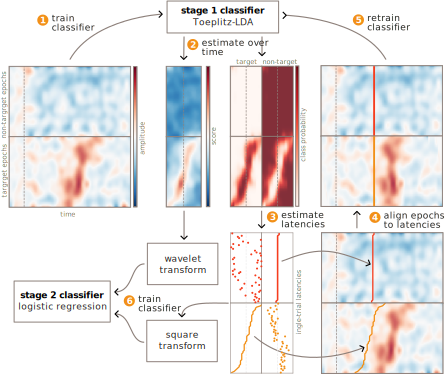
\includegraphics[width=\textwidth]{figures/wcble/figure1.pdf}
}{%
  Schematic representation of the \ac{wcble} training phase.
}{%
  Schematic representation of the \ac{wcble} training phase.
  (1) The first-stage spatiotemporal binary classifier is trained on a set of
  epochs.
  (2) It is	then applied to time-shifted copies of the epochs to obtain scores
  and class probabilities	over time.
  (3) The medians of these probability distributions are assumed the class
  latencies.
  (4) The epochs are aligned to their corresponding	class latencies by
  shifting in time such that all latencies fall at the same moment.
  (5) The spatiotemporal classifier is then retrained on the aligned epochs
  for a	next iteration.
  (6) After the iterative process halts, the scores and	latencies obtained
  from the last iteration are used to train the second-stage
  classifier.
}{%
  fig:diagram-train
}
The process halts after a fixed amount of iterations or when the estimated set
of latencies has been encountered before, indicating it ended up in a loop.
In the end, the procedure should result in enhanced classifier parameters $\theta^*$,
closer to those when there would be no jitter between epochs.
Note that using the median approach for robust latency estimation results in a
smoother yet longer convergence process compared to the maximum/minimum approach.
We can then apply the classifier with enhanced parameters $\theta^*$ in a \ac{cble}
manner to unseen epochs as illustrated in Figure~\ref{fig:diagram-eval} to obtain a
vector of scores over time as in~Section~\ref{sec:cble} and the estimated latencies as
in~Section~\ref{sec:robust-latency}.
\fullpagefig{
  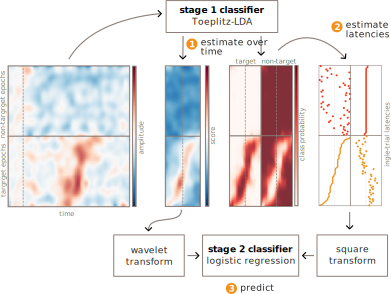
\includegraphics[width=\textwidth]{figures/wcble/figure2.pdf}

}{%
  Schematic representation of the \ac{wcble} test phase.
}{%
  Schematic representation of the Woody Classifier Based Latency
  Estimation test phase. (1) The
	first-stage	spatiotemporal binary classifier obtained from the training phase is
	applied to time-shifted copies of the epochs to obtain scores and class probabilities
	over time. (2) The medians of these probability distributions are assumed
	as the new class latencies. (3) The scores and class latencies are input to the
  trained second-stage classifier, which predicts the label of the epochs.
}{%
  fig:diagram-eval
}
\todo{Pr not italic}
\todo{re-insert comments}

\begin{algorithm}[H]
	\textsc{Train}
	\smallskip \hrule \smallskip
	\textbf{Input:} $\{\mat{X}_n^\mathrm{train}\}_{n=1}^N,
  \mathbf{l}^\mathrm{train}, \mathcal{C}(\cdot,f, \Pr), s_1, s_2$
  \begin{algorithmic}[1]
		\State $\theta \gets
			\mathrm{train}_\mathcal{C}(\{\mat{X}_n^\mathrm{train}[:,s_1:s_2]\}_{n=1}^N,\mathbf{l})$
      %\algorithmiccomment{Train stage 1}
		\For{$n=1\ldots N$}
      %\algorithmiccomment{Feature extraction for stage 2}
		  \For{$s=1\ldots R$}
      \State $y_{n,s}^\mathrm{train} \gets f(\mat{X}_n^\mathrm{train}[:,s:s+(s_2-s_1)],\theta)$
        \EndFor
        \State $s_{n,\mathrm{target}}^\mathrm{train} \gets
			    \mathrm{median}\left[Pr(s|\mat{X}_n^\mathrm{train},\theta,\mathrm{target})\right]$
		    \State $s_{n,\mathrm{non-target}}^\mathrm{train}\gets
			    \mathrm{median}\left[Pr(s|\mat{X}_n^\mathrm{train},\theta,\textrm{non-target})\right]$
    \EndFor
	\end{algorithmic}
  \textbf{Output:} $\theta,
  \mat{Y}^\mathrm{train},
  \mathbf{s}_\mathrm{target}^\mathrm{train},
  \mathbf{s}_\mathrm{non-target}^\mathrm{train}$
	\smallskip \hrule \smallskip
	\textsc{Evaluate}
	\smallskip \hrule \smallskip
	\textbf{Input:} $\{\mat{X}_m^\mathrm{test}\}_{m=1}^N, \mathcal{C}(\theta,f, \Pr), s_1, s_2$
  \begin{algorithmic}[1]
		\For{$m=1\ldots M$}
      %\algorithmiccomment{Feature extraction for stage 2}
		  \For{$s=1\ldots R$}
      \State $y_{m,s}^\mathrm{test} \gets f(\mat{X}_n^\mathrm{test}[:,s:s+(s_2-s_1)],\theta)$
        \EndFor
        \State $s_{m,\mathrm{target}}^\mathrm{test} \gets
			    \mathrm{median}\left[Pr(s|\mat{X}_m^\mathrm{test},\theta,\mathrm{target})\right]$
		    \State $s_{m,\mathrm{non-target}}^\mathrm{test}\gets
			    \mathrm{median}\left[Pr(s|\mat{X}_m^\mathrm{test},\theta,\textrm{non-target})\right]$
    \EndFor
	\end{algorithmic}
  \textbf{Output:} $\mat{Y}^\mathrm{test},
  \mathbf{s}_\mathrm{target}^\mathrm{test},
  \mathbf{s}_\mathrm{non-target}^\mathrm{test}$

  \caption{\Ac{cble}}
	\label{alg:cble}
\end{algorithm}

\begin{algorithm}[H]
	\textsc{Train}
	\smallskip \hrule \smallskip
	\textbf{Input:} $\{\mat{X}_n^\mathrm{train}\}_{n=1}^N, \mathbf{l})
		\mathcal{C}(\cdot,f,\Pr), s_1, s_2$
	\begin{algorithmic}[1]
		\State $\mat{X}'_n \gets \mat{X}^\mathrm{train}_n \quad \forall \quad n=1\ldots
    N$
      %\algorithmiccomment{Train stage 1}
		\Repeat
		\State $\theta^* \gets \mathrm{train}_\mathcal{C}(\{\mat{X}'_n[:,s_1:s_2]\}_0^{N-1},\mathbf{l}$
		\For{$n=1\ldots N$}
    \State  $s_n \gets
			    \mathrm{median}\left[Pr(s|\mat{X}_n',\theta^*,l_n)\right]$
		\State $\mat{X}'_n \gets \mathrm{align}(\mat{X}^\mathrm{train}_n, s^*_n)$
		\EndFor
    \Until{convergence or maximum iterations reached}
    \For{$n=1\ldots N$}%\algorithmiccomment{Feature extraction for stage 2}
		  \For{$s=1\ldots R$}
      \State $y_{n,s}^\mathrm{train} \gets
      f(\mat{X}_n^\mathrm{train}[:,s:s+(s_2-s_1)],\theta^*)$
        \EndFor
        \State $s_{n,\mathrm{target}}^\mathrm{train} \gets
			    \mathrm{median}\left[Pr(s|\mat{X}_n^\mathrm{train},\theta^*,\mathrm{target})\right]$
		    \State $s_{n,\mathrm{non-target}}^\mathrm{train}\gets
			    \mathrm{median}\left[Pr(s|\mat{X}_n^\mathrm{train},\theta^*,\textrm{non-target})\right]$
    \EndFor

	\end{algorithmic}
	\textbf{Output:} $\theta^*,
  \mat{Y}^\mathrm{train},
  \mathbf{s}_\mathrm{target}^\mathrm{train},
  \mathbf{s}_\mathrm{non-target}^\mathrm{train}$

	\smallskip \hrule \smallskip
	\textsc{Evaluate}
	\smallskip \hrule \smallskip
	\textbf{Input:} $\{\mat{X}_m^\mathrm{test}\}_{m=1}^N, \mathcal{C}(\theta^*,f, \Pr), s_1, s_2$
  \begin{algorithmic}[1]
		\For{$m=1\ldots M$}%\algorithmiccomment{Feature extraction for stage 2}
		  \For{$s=1\ldots R$}
      \State $y_{m,s}^\mathrm{test} \gets
      f(\mat{X}_n^\mathrm{test}[:,s:s+(s_2-s_1)],\theta^*)$
        \EndFor
        \State $s_{m,\mathrm{target}}^\mathrm{test} \gets
			    \mathrm{median}\left[Pr(s|\mat{X}_m^\mathrm{test},\theta^*,\mathrm{target})\right]$
		    \State $s_{m,\mathrm{non-target}}^\mathrm{test}\gets
			    \mathrm{median}\left[Pr(s|\mat{X}_m^\mathrm{test},\theta^*,\textrm{non-target})\right]$
    \EndFor
	\end{algorithmic}
  \textbf{Output:} $\mat{Y}^\mathrm{test},
  \mathbf{s}_\mathrm{target}^\mathrm{test},
  \mathbf{s}_\mathrm{non-target}^\mathrm{test}$
  \caption{\ac{wcble}}
	\label{alg:wcble}
\end{algorithm}

\section{Results}
\label{sec:wcble/results}
\todo{refer to later chapter for results on real data}
\subsection{Data simulation}
To verify our approach, we simulated 16 channel \ac{eeg} data with standard
10-20 electrode positions using the \texttt{simulate\_evoked} method of the
MNE (version 1.8)~\cite{Gramfort2013} software package.
\Acp{erp} were generated by projecting a sine wave pulse source time course in a dipole in the
left hemisphere to the scalp electrodes using a boundary element method forward
model~\cite{Mosher1999} MNE's \texttt{fsaverage} source space and anatomy.
Pink temporal noise is generated by passing gaussian noise through an infinite
impulse response filter with transfer function
$\frac{B(z)}{A(z)} = \frac{1}{1 -1z^{-1}+0.15z^{-2}}$.
Pink spatial noise is also added, using a noise covariance matrix constructed from the
cosine distances between electrode positions and scaling it by the inverse of
the resulting spatial.
We refer to~\textcite{Gramfort2014} for implementation details.
%Evoked potentials are simulated for three different source time course waveforms,
%a gaussian, a morlet wavelet and a sinusoid pulse with variable latency,
%defined by the following formulas:
%\begin{equation}
%  f_\text{gaussian}(t,l) = a
%  \frac{1}{\varsigma\sqrt{2\pi}}e^{-\frac{1}{2}\frac{\left(t-l\right)^2}{\varsigma/2}}
%\end{equation}
%\begin{equation}
%  f_\text{morlet}(t,l) = ae^{-\left(\frac{t-l}{\frac{c}{2\pi f}}\right)^2}
%\end{equation}
The source time course is defined by the following function:
\begin{equation}
  s(t,l) =
  \begin{cases}
    a\sin\left(2\pi f\left(t-l\right)\right) & \text{if  $l-\frac{1}{2f} < t < l-\frac{1}{2f}$} \\
    0 & \text{otherwise}
  \end{cases}
\end{equation}
over time $t$, with latency $l$ and amplitude $a=\num{1e{-7}}$V and frequency
$f=4$.
%The standard deviation that determines the width gaussian $\varsigma=0.1s$.
%For the morlet wavelet, the number of cycles $c=3$ and the frequency $f=4Hz$.
%For the sine pulse, the frequency $f=4$

%For each of these,
100 target epochs containing the evoked potential and noise and 100
non-target epochs containing only noise were simulated.
The target epochs were jittered by setting the latency offset $l$
of each target epoch to a random latency drawn from a normal distribution with 0 mean and standard
deviations of respectively $\sigma=0.1,0.2,0.3$s.
The noise was scaled at different 32  different noise levels, with the \ac{snr} of a
target epoch ranging from 0 to -31dB, with
\begin{equation}
  \text{SNR} = 10\log_{10}\frac{\text{var}s(t,0)}{\text{var}\left(\text{noise}\right)}
\end{equation}

%A sample of the simulated evoked data is displayed in Figures~\ref{fig:wcble/sim-gausian}, \ref{fig:wcble/sim-morlet} and
A sample of the simulated evoked data is displayed in Figures~\ref{fig:wcble/sim-sine}.
%\fullpagefig{figures/wcble/simulated-gaussian.pdf}{}{fig:wcble/sim-gaussian}
%\fullpagefig{figures/wcble/simulated-morlet.pdf}{}{fig:wcble/sim-morlet}
\fullpagefig{%
  \includegraphics[width=\textwidth]{figures/wcble/simulated-sine.pdf}
}{%
  Simulated target and non-target evoked data.
}{%
  Simulated target and non-target evoked data. Targets contain a sine wave
  pulse jittered by $\sigma$. 32 EEG channels with pink
  spatiotemporal noise were simulated using a forward head model, channel C3 is
  plotted here.
}{fig:wcble/sim-sine}
\todo{Properly align plots and label axes}
\todo{decrease tick size}

\subsection{Latency estimation}
\todo{refer to figure}
We compared our proposed \ac{wcble} algorithm to \ac{cble} on a latency
estimation task using the pearson correlation coefficient $\rho$\todo{equation} at different
jitter and \ac{snr} levels.
For both \ac{cble} and \ac{wcble}, target latencies where extracted in a
10-fold cross-validation scheme using the robust median latency method after
fitting the model.
\Ac{wcble}'s maximum iteration number was set to 64.
Results are presented in Figure~\ref{fig:wcble/results/latency}.
A 95\ confidence intervals on each measure was obtained through bootstrapping
with 1000 permutations.

\begin{figure}[!ht]
  %% Creator: Matplotlib, PGF backend
%%
%% To include the figure in your LaTeX document, write
%%   \input{<filename>.pgf}
%%
%% Make sure the required packages are loaded in your preamble
%%   \usepackage{pgf}
%%
%% Also ensure that all the required font packages are loaded; for instance,
%% the lmodern package is sometimes necessary when using math font.
%%   \usepackage{lmodern}
%%
%% Figures using additional raster images can only be included by \input if
%% they are in the same directory as the main LaTeX file. For loading figures
%% from other directories you can use the `import` package
%%   \usepackage{import}
%%
%% and then include the figures with
%%   \import{<path to file>}{<filename>.pgf}
%%
%% Matplotlib used the following preamble
%%   \def\mathdefault#1{#1}
%%   \everymath=\expandafter{\the\everymath\displaystyle}
%%   
%%   \ifdefined\pdftexversion\else  % non-pdftex case.
%%     \usepackage{fontspec}
%%   \fi
%%   \makeatletter\@ifpackageloaded{underscore}{}{\usepackage[strings]{underscore}}\makeatother
%%
\begingroup%
\makeatletter%
\begin{pgfpicture}%
\pgfpathrectangle{\pgfpointorigin}{\pgfqpoint{6.642116in}{1.634668in}}%
\pgfusepath{use as bounding box, clip}%
\begin{pgfscope}%
\pgfsetbuttcap%
\pgfsetmiterjoin%
\definecolor{currentfill}{rgb}{1.000000,1.000000,1.000000}%
\pgfsetfillcolor{currentfill}%
\pgfsetlinewidth{0.000000pt}%
\definecolor{currentstroke}{rgb}{1.000000,1.000000,1.000000}%
\pgfsetstrokecolor{currentstroke}%
\pgfsetdash{}{0pt}%
\pgfpathmoveto{\pgfqpoint{0.000000in}{0.000000in}}%
\pgfpathlineto{\pgfqpoint{6.642116in}{0.000000in}}%
\pgfpathlineto{\pgfqpoint{6.642116in}{1.634668in}}%
\pgfpathlineto{\pgfqpoint{0.000000in}{1.634668in}}%
\pgfpathlineto{\pgfqpoint{0.000000in}{0.000000in}}%
\pgfpathclose%
\pgfusepath{fill}%
\end{pgfscope}%
\begin{pgfscope}%
\pgfsetbuttcap%
\pgfsetmiterjoin%
\definecolor{currentfill}{rgb}{1.000000,1.000000,1.000000}%
\pgfsetfillcolor{currentfill}%
\pgfsetlinewidth{0.000000pt}%
\definecolor{currentstroke}{rgb}{0.000000,0.000000,0.000000}%
\pgfsetstrokecolor{currentstroke}%
\pgfsetstrokeopacity{0.000000}%
\pgfsetdash{}{0pt}%
\pgfpathmoveto{\pgfqpoint{0.443671in}{0.340278in}}%
\pgfpathlineto{\pgfqpoint{2.287577in}{0.340278in}}%
\pgfpathlineto{\pgfqpoint{2.287577in}{1.464529in}}%
\pgfpathlineto{\pgfqpoint{0.443671in}{1.464529in}}%
\pgfpathlineto{\pgfqpoint{0.443671in}{0.340278in}}%
\pgfpathclose%
\pgfusepath{fill}%
\end{pgfscope}%
\begin{pgfscope}%
\pgfpathrectangle{\pgfqpoint{0.443671in}{0.340278in}}{\pgfqpoint{1.843905in}{1.124251in}}%
\pgfusepath{clip}%
\pgfsetbuttcap%
\pgfsetroundjoin%
\definecolor{currentfill}{rgb}{0.949020,0.564706,0.094118}%
\pgfsetfillcolor{currentfill}%
\pgfsetfillopacity{0.200000}%
\pgfsetlinewidth{1.003750pt}%
\definecolor{currentstroke}{rgb}{0.949020,0.564706,0.094118}%
\pgfsetstrokecolor{currentstroke}%
\pgfsetstrokeopacity{0.200000}%
\pgfsetdash{}{0pt}%
\pgfsys@defobject{currentmarker}{\pgfqpoint{0.443671in}{0.321126in}}{\pgfqpoint{2.287577in}{1.452076in}}{%
\pgfpathmoveto{\pgfqpoint{2.287577in}{0.871109in}}%
\pgfpathlineto{\pgfqpoint{2.287577in}{0.321126in}}%
\pgfpathlineto{\pgfqpoint{2.228096in}{0.333038in}}%
\pgfpathlineto{\pgfqpoint{2.168615in}{0.565105in}}%
\pgfpathlineto{\pgfqpoint{2.109134in}{0.548990in}}%
\pgfpathlineto{\pgfqpoint{2.049653in}{0.618005in}}%
\pgfpathlineto{\pgfqpoint{1.990173in}{0.788456in}}%
\pgfpathlineto{\pgfqpoint{1.930692in}{0.846366in}}%
\pgfpathlineto{\pgfqpoint{1.871211in}{1.068636in}}%
\pgfpathlineto{\pgfqpoint{1.811730in}{1.066712in}}%
\pgfpathlineto{\pgfqpoint{1.752249in}{1.224783in}}%
\pgfpathlineto{\pgfqpoint{1.692769in}{1.437673in}}%
\pgfpathlineto{\pgfqpoint{1.633288in}{1.437897in}}%
\pgfpathlineto{\pgfqpoint{1.573807in}{1.437307in}}%
\pgfpathlineto{\pgfqpoint{1.514326in}{1.431312in}}%
\pgfpathlineto{\pgfqpoint{1.454845in}{1.432787in}}%
\pgfpathlineto{\pgfqpoint{1.395364in}{1.439969in}}%
\pgfpathlineto{\pgfqpoint{1.335884in}{1.440120in}}%
\pgfpathlineto{\pgfqpoint{1.276403in}{1.435007in}}%
\pgfpathlineto{\pgfqpoint{1.216922in}{1.435134in}}%
\pgfpathlineto{\pgfqpoint{1.157441in}{1.434364in}}%
\pgfpathlineto{\pgfqpoint{1.097960in}{1.432797in}}%
\pgfpathlineto{\pgfqpoint{1.038480in}{1.432869in}}%
\pgfpathlineto{\pgfqpoint{0.978999in}{1.427345in}}%
\pgfpathlineto{\pgfqpoint{0.919518in}{1.426838in}}%
\pgfpathlineto{\pgfqpoint{0.860037in}{1.426990in}}%
\pgfpathlineto{\pgfqpoint{0.800556in}{1.425104in}}%
\pgfpathlineto{\pgfqpoint{0.741075in}{1.423211in}}%
\pgfpathlineto{\pgfqpoint{0.681595in}{1.421917in}}%
\pgfpathlineto{\pgfqpoint{0.622114in}{1.425895in}}%
\pgfpathlineto{\pgfqpoint{0.562633in}{1.426784in}}%
\pgfpathlineto{\pgfqpoint{0.503152in}{1.426714in}}%
\pgfpathlineto{\pgfqpoint{0.443671in}{1.422863in}}%
\pgfpathlineto{\pgfqpoint{0.443671in}{1.451165in}}%
\pgfpathlineto{\pgfqpoint{0.443671in}{1.451165in}}%
\pgfpathlineto{\pgfqpoint{0.503152in}{1.452019in}}%
\pgfpathlineto{\pgfqpoint{0.562633in}{1.452076in}}%
\pgfpathlineto{\pgfqpoint{0.622114in}{1.449737in}}%
\pgfpathlineto{\pgfqpoint{0.681595in}{1.449031in}}%
\pgfpathlineto{\pgfqpoint{0.741075in}{1.449014in}}%
\pgfpathlineto{\pgfqpoint{0.800556in}{1.448567in}}%
\pgfpathlineto{\pgfqpoint{0.860037in}{1.450176in}}%
\pgfpathlineto{\pgfqpoint{0.919518in}{1.449770in}}%
\pgfpathlineto{\pgfqpoint{0.978999in}{1.450239in}}%
\pgfpathlineto{\pgfqpoint{1.038480in}{1.450150in}}%
\pgfpathlineto{\pgfqpoint{1.097960in}{1.450810in}}%
\pgfpathlineto{\pgfqpoint{1.157441in}{1.450515in}}%
\pgfpathlineto{\pgfqpoint{1.216922in}{1.449766in}}%
\pgfpathlineto{\pgfqpoint{1.276403in}{1.449490in}}%
\pgfpathlineto{\pgfqpoint{1.335884in}{1.450104in}}%
\pgfpathlineto{\pgfqpoint{1.395364in}{1.449868in}}%
\pgfpathlineto{\pgfqpoint{1.454845in}{1.448718in}}%
\pgfpathlineto{\pgfqpoint{1.514326in}{1.448310in}}%
\pgfpathlineto{\pgfqpoint{1.573807in}{1.448030in}}%
\pgfpathlineto{\pgfqpoint{1.633288in}{1.448341in}}%
\pgfpathlineto{\pgfqpoint{1.692769in}{1.447805in}}%
\pgfpathlineto{\pgfqpoint{1.752249in}{1.442848in}}%
\pgfpathlineto{\pgfqpoint{1.811730in}{1.433072in}}%
\pgfpathlineto{\pgfqpoint{1.871211in}{1.431081in}}%
\pgfpathlineto{\pgfqpoint{1.930692in}{1.272105in}}%
\pgfpathlineto{\pgfqpoint{1.990173in}{1.149301in}}%
\pgfpathlineto{\pgfqpoint{2.049653in}{1.117425in}}%
\pgfpathlineto{\pgfqpoint{2.109134in}{1.090927in}}%
\pgfpathlineto{\pgfqpoint{2.168615in}{1.034962in}}%
\pgfpathlineto{\pgfqpoint{2.228096in}{0.910750in}}%
\pgfpathlineto{\pgfqpoint{2.287577in}{0.871109in}}%
\pgfpathlineto{\pgfqpoint{2.287577in}{0.871109in}}%
\pgfpathclose%
\pgfusepath{stroke,fill}%
}%
\begin{pgfscope}%
\pgfsys@transformshift{0.000000in}{0.000000in}%
\pgfsys@useobject{currentmarker}{}%
\end{pgfscope}%
\end{pgfscope}%
\begin{pgfscope}%
\pgfpathrectangle{\pgfqpoint{0.443671in}{0.340278in}}{\pgfqpoint{1.843905in}{1.124251in}}%
\pgfusepath{clip}%
\pgfsetbuttcap%
\pgfsetroundjoin%
\definecolor{currentfill}{rgb}{0.964706,0.239216,0.117647}%
\pgfsetfillcolor{currentfill}%
\pgfsetfillopacity{0.200000}%
\pgfsetlinewidth{1.003750pt}%
\definecolor{currentstroke}{rgb}{0.964706,0.239216,0.117647}%
\pgfsetstrokecolor{currentstroke}%
\pgfsetstrokeopacity{0.200000}%
\pgfsetdash{}{0pt}%
\pgfsys@defobject{currentmarker}{\pgfqpoint{0.443671in}{0.294673in}}{\pgfqpoint{2.287577in}{1.461663in}}{%
\pgfpathmoveto{\pgfqpoint{2.287577in}{0.822164in}}%
\pgfpathlineto{\pgfqpoint{2.287577in}{0.294673in}}%
\pgfpathlineto{\pgfqpoint{2.228096in}{0.514588in}}%
\pgfpathlineto{\pgfqpoint{2.168615in}{0.844883in}}%
\pgfpathlineto{\pgfqpoint{2.109134in}{1.046871in}}%
\pgfpathlineto{\pgfqpoint{2.049653in}{1.450439in}}%
\pgfpathlineto{\pgfqpoint{1.990173in}{1.447690in}}%
\pgfpathlineto{\pgfqpoint{1.930692in}{1.457224in}}%
\pgfpathlineto{\pgfqpoint{1.871211in}{1.455777in}}%
\pgfpathlineto{\pgfqpoint{1.811730in}{1.452490in}}%
\pgfpathlineto{\pgfqpoint{1.752249in}{1.452310in}}%
\pgfpathlineto{\pgfqpoint{1.692769in}{1.452776in}}%
\pgfpathlineto{\pgfqpoint{1.633288in}{1.454668in}}%
\pgfpathlineto{\pgfqpoint{1.573807in}{1.455378in}}%
\pgfpathlineto{\pgfqpoint{1.514326in}{1.455354in}}%
\pgfpathlineto{\pgfqpoint{1.454845in}{1.456409in}}%
\pgfpathlineto{\pgfqpoint{1.395364in}{1.455338in}}%
\pgfpathlineto{\pgfqpoint{1.335884in}{1.456637in}}%
\pgfpathlineto{\pgfqpoint{1.276403in}{1.457826in}}%
\pgfpathlineto{\pgfqpoint{1.216922in}{1.457181in}}%
\pgfpathlineto{\pgfqpoint{1.157441in}{1.456426in}}%
\pgfpathlineto{\pgfqpoint{1.097960in}{1.456893in}}%
\pgfpathlineto{\pgfqpoint{1.038480in}{1.457026in}}%
\pgfpathlineto{\pgfqpoint{0.978999in}{1.457318in}}%
\pgfpathlineto{\pgfqpoint{0.919518in}{1.456555in}}%
\pgfpathlineto{\pgfqpoint{0.860037in}{1.457377in}}%
\pgfpathlineto{\pgfqpoint{0.800556in}{1.456014in}}%
\pgfpathlineto{\pgfqpoint{0.741075in}{1.456792in}}%
\pgfpathlineto{\pgfqpoint{0.681595in}{1.457104in}}%
\pgfpathlineto{\pgfqpoint{0.622114in}{1.458297in}}%
\pgfpathlineto{\pgfqpoint{0.562633in}{1.458082in}}%
\pgfpathlineto{\pgfqpoint{0.503152in}{1.457361in}}%
\pgfpathlineto{\pgfqpoint{0.443671in}{1.458175in}}%
\pgfpathlineto{\pgfqpoint{0.443671in}{1.460593in}}%
\pgfpathlineto{\pgfqpoint{0.443671in}{1.460593in}}%
\pgfpathlineto{\pgfqpoint{0.503152in}{1.460280in}}%
\pgfpathlineto{\pgfqpoint{0.562633in}{1.460887in}}%
\pgfpathlineto{\pgfqpoint{0.622114in}{1.460399in}}%
\pgfpathlineto{\pgfqpoint{0.681595in}{1.460296in}}%
\pgfpathlineto{\pgfqpoint{0.741075in}{1.459635in}}%
\pgfpathlineto{\pgfqpoint{0.800556in}{1.459829in}}%
\pgfpathlineto{\pgfqpoint{0.860037in}{1.460488in}}%
\pgfpathlineto{\pgfqpoint{0.919518in}{1.460529in}}%
\pgfpathlineto{\pgfqpoint{0.978999in}{1.460260in}}%
\pgfpathlineto{\pgfqpoint{1.038480in}{1.459732in}}%
\pgfpathlineto{\pgfqpoint{1.097960in}{1.460387in}}%
\pgfpathlineto{\pgfqpoint{1.157441in}{1.460173in}}%
\pgfpathlineto{\pgfqpoint{1.216922in}{1.460688in}}%
\pgfpathlineto{\pgfqpoint{1.276403in}{1.461181in}}%
\pgfpathlineto{\pgfqpoint{1.335884in}{1.460500in}}%
\pgfpathlineto{\pgfqpoint{1.395364in}{1.459827in}}%
\pgfpathlineto{\pgfqpoint{1.454845in}{1.460768in}}%
\pgfpathlineto{\pgfqpoint{1.514326in}{1.461663in}}%
\pgfpathlineto{\pgfqpoint{1.573807in}{1.460741in}}%
\pgfpathlineto{\pgfqpoint{1.633288in}{1.459337in}}%
\pgfpathlineto{\pgfqpoint{1.692769in}{1.458815in}}%
\pgfpathlineto{\pgfqpoint{1.752249in}{1.458617in}}%
\pgfpathlineto{\pgfqpoint{1.811730in}{1.459054in}}%
\pgfpathlineto{\pgfqpoint{1.871211in}{1.459181in}}%
\pgfpathlineto{\pgfqpoint{1.930692in}{1.460096in}}%
\pgfpathlineto{\pgfqpoint{1.990173in}{1.456266in}}%
\pgfpathlineto{\pgfqpoint{2.049653in}{1.456828in}}%
\pgfpathlineto{\pgfqpoint{2.109134in}{1.449151in}}%
\pgfpathlineto{\pgfqpoint{2.168615in}{1.440019in}}%
\pgfpathlineto{\pgfqpoint{2.228096in}{1.113076in}}%
\pgfpathlineto{\pgfqpoint{2.287577in}{0.822164in}}%
\pgfpathlineto{\pgfqpoint{2.287577in}{0.822164in}}%
\pgfpathclose%
\pgfusepath{stroke,fill}%
}%
\begin{pgfscope}%
\pgfsys@transformshift{0.000000in}{0.000000in}%
\pgfsys@useobject{currentmarker}{}%
\end{pgfscope}%
\end{pgfscope}%
\begin{pgfscope}%
\pgfsetbuttcap%
\pgfsetroundjoin%
\definecolor{currentfill}{rgb}{0.552941,0.501961,0.478431}%
\pgfsetfillcolor{currentfill}%
\pgfsetlinewidth{0.803000pt}%
\definecolor{currentstroke}{rgb}{0.552941,0.501961,0.478431}%
\pgfsetstrokecolor{currentstroke}%
\pgfsetdash{}{0pt}%
\pgfsys@defobject{currentmarker}{\pgfqpoint{0.000000in}{0.000000in}}{\pgfqpoint{0.000000in}{0.083333in}}{%
\pgfpathmoveto{\pgfqpoint{0.000000in}{0.000000in}}%
\pgfpathlineto{\pgfqpoint{0.000000in}{0.083333in}}%
\pgfusepath{stroke,fill}%
}%
\begin{pgfscope}%
\pgfsys@transformshift{2.228096in}{0.340278in}%
\pgfsys@useobject{currentmarker}{}%
\end{pgfscope}%
\end{pgfscope}%
\begin{pgfscope}%
\definecolor{textcolor}{rgb}{0.552941,0.501961,0.478431}%
\pgfsetstrokecolor{textcolor}%
\pgfsetfillcolor{textcolor}%
\pgftext[x=2.228096in,y=0.291667in,,top]{\color{textcolor}{\sffamily\fontsize{9.000000}{10.800000}\selectfont\catcode`\^=\active\def^{\ifmmode\sp\else\^{}\fi}\catcode`\%=\active\def%{\%}$\mathdefault{\ensuremath{-}30}$}}%
\end{pgfscope}%
\begin{pgfscope}%
\pgfsetbuttcap%
\pgfsetroundjoin%
\definecolor{currentfill}{rgb}{0.552941,0.501961,0.478431}%
\pgfsetfillcolor{currentfill}%
\pgfsetlinewidth{0.803000pt}%
\definecolor{currentstroke}{rgb}{0.552941,0.501961,0.478431}%
\pgfsetstrokecolor{currentstroke}%
\pgfsetdash{}{0pt}%
\pgfsys@defobject{currentmarker}{\pgfqpoint{0.000000in}{0.000000in}}{\pgfqpoint{0.000000in}{0.083333in}}{%
\pgfpathmoveto{\pgfqpoint{0.000000in}{0.000000in}}%
\pgfpathlineto{\pgfqpoint{0.000000in}{0.083333in}}%
\pgfusepath{stroke,fill}%
}%
\begin{pgfscope}%
\pgfsys@transformshift{1.633288in}{0.340278in}%
\pgfsys@useobject{currentmarker}{}%
\end{pgfscope}%
\end{pgfscope}%
\begin{pgfscope}%
\definecolor{textcolor}{rgb}{0.552941,0.501961,0.478431}%
\pgfsetstrokecolor{textcolor}%
\pgfsetfillcolor{textcolor}%
\pgftext[x=1.633288in,y=0.291667in,,top]{\color{textcolor}{\sffamily\fontsize{9.000000}{10.800000}\selectfont\catcode`\^=\active\def^{\ifmmode\sp\else\^{}\fi}\catcode`\%=\active\def%{\%}$\mathdefault{\ensuremath{-}20}$}}%
\end{pgfscope}%
\begin{pgfscope}%
\pgfsetbuttcap%
\pgfsetroundjoin%
\definecolor{currentfill}{rgb}{0.552941,0.501961,0.478431}%
\pgfsetfillcolor{currentfill}%
\pgfsetlinewidth{0.803000pt}%
\definecolor{currentstroke}{rgb}{0.552941,0.501961,0.478431}%
\pgfsetstrokecolor{currentstroke}%
\pgfsetdash{}{0pt}%
\pgfsys@defobject{currentmarker}{\pgfqpoint{0.000000in}{0.000000in}}{\pgfqpoint{0.000000in}{0.083333in}}{%
\pgfpathmoveto{\pgfqpoint{0.000000in}{0.000000in}}%
\pgfpathlineto{\pgfqpoint{0.000000in}{0.083333in}}%
\pgfusepath{stroke,fill}%
}%
\begin{pgfscope}%
\pgfsys@transformshift{1.038480in}{0.340278in}%
\pgfsys@useobject{currentmarker}{}%
\end{pgfscope}%
\end{pgfscope}%
\begin{pgfscope}%
\definecolor{textcolor}{rgb}{0.552941,0.501961,0.478431}%
\pgfsetstrokecolor{textcolor}%
\pgfsetfillcolor{textcolor}%
\pgftext[x=1.038480in,y=0.291667in,,top]{\color{textcolor}{\sffamily\fontsize{9.000000}{10.800000}\selectfont\catcode`\^=\active\def^{\ifmmode\sp\else\^{}\fi}\catcode`\%=\active\def%{\%}$\mathdefault{\ensuremath{-}10}$}}%
\end{pgfscope}%
\begin{pgfscope}%
\pgfsetbuttcap%
\pgfsetroundjoin%
\definecolor{currentfill}{rgb}{0.552941,0.501961,0.478431}%
\pgfsetfillcolor{currentfill}%
\pgfsetlinewidth{0.803000pt}%
\definecolor{currentstroke}{rgb}{0.552941,0.501961,0.478431}%
\pgfsetstrokecolor{currentstroke}%
\pgfsetdash{}{0pt}%
\pgfsys@defobject{currentmarker}{\pgfqpoint{0.000000in}{0.000000in}}{\pgfqpoint{0.000000in}{0.083333in}}{%
\pgfpathmoveto{\pgfqpoint{0.000000in}{0.000000in}}%
\pgfpathlineto{\pgfqpoint{0.000000in}{0.083333in}}%
\pgfusepath{stroke,fill}%
}%
\begin{pgfscope}%
\pgfsys@transformshift{0.443671in}{0.340278in}%
\pgfsys@useobject{currentmarker}{}%
\end{pgfscope}%
\end{pgfscope}%
\begin{pgfscope}%
\definecolor{textcolor}{rgb}{0.552941,0.501961,0.478431}%
\pgfsetstrokecolor{textcolor}%
\pgfsetfillcolor{textcolor}%
\pgftext[x=0.443671in,y=0.291667in,,top]{\color{textcolor}{\sffamily\fontsize{9.000000}{10.800000}\selectfont\catcode`\^=\active\def^{\ifmmode\sp\else\^{}\fi}\catcode`\%=\active\def%{\%}$\mathdefault{0}$}}%
\end{pgfscope}%
\begin{pgfscope}%
\definecolor{textcolor}{rgb}{0.552941,0.501961,0.478431}%
\pgfsetstrokecolor{textcolor}%
\pgfsetfillcolor{textcolor}%
\pgftext[x=1.365624in,y=0.125000in,,top]{\color{textcolor}{\sffamily\fontsize{9.000000}{10.800000}\selectfont\catcode`\^=\active\def^{\ifmmode\sp\else\^{}\fi}\catcode`\%=\active\def%{\%}SNR (dB)}}%
\end{pgfscope}%
\begin{pgfscope}%
\pgfsetbuttcap%
\pgfsetroundjoin%
\definecolor{currentfill}{rgb}{0.552941,0.501961,0.478431}%
\pgfsetfillcolor{currentfill}%
\pgfsetlinewidth{0.803000pt}%
\definecolor{currentstroke}{rgb}{0.552941,0.501961,0.478431}%
\pgfsetstrokecolor{currentstroke}%
\pgfsetdash{}{0pt}%
\pgfsys@defobject{currentmarker}{\pgfqpoint{0.000000in}{0.000000in}}{\pgfqpoint{0.083333in}{0.000000in}}{%
\pgfpathmoveto{\pgfqpoint{0.000000in}{0.000000in}}%
\pgfpathlineto{\pgfqpoint{0.083333in}{0.000000in}}%
\pgfusepath{stroke,fill}%
}%
\begin{pgfscope}%
\pgfsys@transformshift{0.443671in}{0.340278in}%
\pgfsys@useobject{currentmarker}{}%
\end{pgfscope}%
\end{pgfscope}%
\begin{pgfscope}%
\definecolor{textcolor}{rgb}{0.552941,0.501961,0.478431}%
\pgfsetstrokecolor{textcolor}%
\pgfsetfillcolor{textcolor}%
\pgftext[x=0.166667in, y=0.296875in, left, base]{\color{textcolor}{\sffamily\fontsize{9.000000}{10.800000}\selectfont\catcode`\^=\active\def^{\ifmmode\sp\else\^{}\fi}\catcode`\%=\active\def%{\%}$\mathdefault{0.00}$}}%
\end{pgfscope}%
\begin{pgfscope}%
\pgfsetbuttcap%
\pgfsetroundjoin%
\definecolor{currentfill}{rgb}{0.552941,0.501961,0.478431}%
\pgfsetfillcolor{currentfill}%
\pgfsetlinewidth{0.803000pt}%
\definecolor{currentstroke}{rgb}{0.552941,0.501961,0.478431}%
\pgfsetstrokecolor{currentstroke}%
\pgfsetdash{}{0pt}%
\pgfsys@defobject{currentmarker}{\pgfqpoint{0.000000in}{0.000000in}}{\pgfqpoint{0.083333in}{0.000000in}}{%
\pgfpathmoveto{\pgfqpoint{0.000000in}{0.000000in}}%
\pgfpathlineto{\pgfqpoint{0.083333in}{0.000000in}}%
\pgfusepath{stroke,fill}%
}%
\begin{pgfscope}%
\pgfsys@transformshift{0.443671in}{0.621341in}%
\pgfsys@useobject{currentmarker}{}%
\end{pgfscope}%
\end{pgfscope}%
\begin{pgfscope}%
\definecolor{textcolor}{rgb}{0.552941,0.501961,0.478431}%
\pgfsetstrokecolor{textcolor}%
\pgfsetfillcolor{textcolor}%
\pgftext[x=0.166667in, y=0.577938in, left, base]{\color{textcolor}{\sffamily\fontsize{9.000000}{10.800000}\selectfont\catcode`\^=\active\def^{\ifmmode\sp\else\^{}\fi}\catcode`\%=\active\def%{\%}$\mathdefault{0.25}$}}%
\end{pgfscope}%
\begin{pgfscope}%
\pgfsetbuttcap%
\pgfsetroundjoin%
\definecolor{currentfill}{rgb}{0.552941,0.501961,0.478431}%
\pgfsetfillcolor{currentfill}%
\pgfsetlinewidth{0.803000pt}%
\definecolor{currentstroke}{rgb}{0.552941,0.501961,0.478431}%
\pgfsetstrokecolor{currentstroke}%
\pgfsetdash{}{0pt}%
\pgfsys@defobject{currentmarker}{\pgfqpoint{0.000000in}{0.000000in}}{\pgfqpoint{0.083333in}{0.000000in}}{%
\pgfpathmoveto{\pgfqpoint{0.000000in}{0.000000in}}%
\pgfpathlineto{\pgfqpoint{0.083333in}{0.000000in}}%
\pgfusepath{stroke,fill}%
}%
\begin{pgfscope}%
\pgfsys@transformshift{0.443671in}{0.902403in}%
\pgfsys@useobject{currentmarker}{}%
\end{pgfscope}%
\end{pgfscope}%
\begin{pgfscope}%
\definecolor{textcolor}{rgb}{0.552941,0.501961,0.478431}%
\pgfsetstrokecolor{textcolor}%
\pgfsetfillcolor{textcolor}%
\pgftext[x=0.166667in, y=0.859001in, left, base]{\color{textcolor}{\sffamily\fontsize{9.000000}{10.800000}\selectfont\catcode`\^=\active\def^{\ifmmode\sp\else\^{}\fi}\catcode`\%=\active\def%{\%}$\mathdefault{0.50}$}}%
\end{pgfscope}%
\begin{pgfscope}%
\pgfsetbuttcap%
\pgfsetroundjoin%
\definecolor{currentfill}{rgb}{0.552941,0.501961,0.478431}%
\pgfsetfillcolor{currentfill}%
\pgfsetlinewidth{0.803000pt}%
\definecolor{currentstroke}{rgb}{0.552941,0.501961,0.478431}%
\pgfsetstrokecolor{currentstroke}%
\pgfsetdash{}{0pt}%
\pgfsys@defobject{currentmarker}{\pgfqpoint{0.000000in}{0.000000in}}{\pgfqpoint{0.083333in}{0.000000in}}{%
\pgfpathmoveto{\pgfqpoint{0.000000in}{0.000000in}}%
\pgfpathlineto{\pgfqpoint{0.083333in}{0.000000in}}%
\pgfusepath{stroke,fill}%
}%
\begin{pgfscope}%
\pgfsys@transformshift{0.443671in}{1.183466in}%
\pgfsys@useobject{currentmarker}{}%
\end{pgfscope}%
\end{pgfscope}%
\begin{pgfscope}%
\definecolor{textcolor}{rgb}{0.552941,0.501961,0.478431}%
\pgfsetstrokecolor{textcolor}%
\pgfsetfillcolor{textcolor}%
\pgftext[x=0.166667in, y=1.140063in, left, base]{\color{textcolor}{\sffamily\fontsize{9.000000}{10.800000}\selectfont\catcode`\^=\active\def^{\ifmmode\sp\else\^{}\fi}\catcode`\%=\active\def%{\%}$\mathdefault{0.75}$}}%
\end{pgfscope}%
\begin{pgfscope}%
\pgfsetbuttcap%
\pgfsetroundjoin%
\definecolor{currentfill}{rgb}{0.552941,0.501961,0.478431}%
\pgfsetfillcolor{currentfill}%
\pgfsetlinewidth{0.803000pt}%
\definecolor{currentstroke}{rgb}{0.552941,0.501961,0.478431}%
\pgfsetstrokecolor{currentstroke}%
\pgfsetdash{}{0pt}%
\pgfsys@defobject{currentmarker}{\pgfqpoint{0.000000in}{0.000000in}}{\pgfqpoint{0.083333in}{0.000000in}}{%
\pgfpathmoveto{\pgfqpoint{0.000000in}{0.000000in}}%
\pgfpathlineto{\pgfqpoint{0.083333in}{0.000000in}}%
\pgfusepath{stroke,fill}%
}%
\begin{pgfscope}%
\pgfsys@transformshift{0.443671in}{1.464529in}%
\pgfsys@useobject{currentmarker}{}%
\end{pgfscope}%
\end{pgfscope}%
\begin{pgfscope}%
\definecolor{textcolor}{rgb}{0.552941,0.501961,0.478431}%
\pgfsetstrokecolor{textcolor}%
\pgfsetfillcolor{textcolor}%
\pgftext[x=0.166667in, y=1.421126in, left, base]{\color{textcolor}{\sffamily\fontsize{9.000000}{10.800000}\selectfont\catcode`\^=\active\def^{\ifmmode\sp\else\^{}\fi}\catcode`\%=\active\def%{\%}$\mathdefault{1.00}$}}%
\end{pgfscope}%
\begin{pgfscope}%
\definecolor{textcolor}{rgb}{0.552941,0.501961,0.478431}%
\pgfsetstrokecolor{textcolor}%
\pgfsetfillcolor{textcolor}%
\pgftext[x=0.111111in,y=0.902403in,,bottom,rotate=90.000000]{\color{textcolor}{\sffamily\fontsize{9.000000}{10.800000}\selectfont\catcode`\^=\active\def^{\ifmmode\sp\else\^{}\fi}\catcode`\%=\active\def%{\%}$\rho$}}%
\end{pgfscope}%
\begin{pgfscope}%
\pgfpathrectangle{\pgfqpoint{0.443671in}{0.340278in}}{\pgfqpoint{1.843905in}{1.124251in}}%
\pgfusepath{clip}%
\pgfsetrectcap%
\pgfsetroundjoin%
\pgfsetlinewidth{1.505625pt}%
\definecolor{currentstroke}{rgb}{0.949020,0.564706,0.094118}%
\pgfsetstrokecolor{currentstroke}%
\pgfsetdash{}{0pt}%
\pgfpathmoveto{\pgfqpoint{2.287577in}{0.605803in}}%
\pgfpathlineto{\pgfqpoint{2.228096in}{0.651300in}}%
\pgfpathlineto{\pgfqpoint{2.168615in}{0.795406in}}%
\pgfpathlineto{\pgfqpoint{2.109134in}{0.828009in}}%
\pgfpathlineto{\pgfqpoint{2.049653in}{0.866514in}}%
\pgfpathlineto{\pgfqpoint{1.990173in}{0.960029in}}%
\pgfpathlineto{\pgfqpoint{1.930692in}{1.055916in}}%
\pgfpathlineto{\pgfqpoint{1.871211in}{1.281280in}}%
\pgfpathlineto{\pgfqpoint{1.811730in}{1.284866in}}%
\pgfpathlineto{\pgfqpoint{1.752249in}{1.367897in}}%
\pgfpathlineto{\pgfqpoint{1.692769in}{1.442989in}}%
\pgfpathlineto{\pgfqpoint{1.633288in}{1.443618in}}%
\pgfpathlineto{\pgfqpoint{1.573807in}{1.442644in}}%
\pgfpathlineto{\pgfqpoint{1.514326in}{1.440673in}}%
\pgfpathlineto{\pgfqpoint{1.454845in}{1.441510in}}%
\pgfpathlineto{\pgfqpoint{1.395364in}{1.444617in}}%
\pgfpathlineto{\pgfqpoint{1.335884in}{1.444617in}}%
\pgfpathlineto{\pgfqpoint{1.276403in}{1.442339in}}%
\pgfpathlineto{\pgfqpoint{1.216922in}{1.442886in}}%
\pgfpathlineto{\pgfqpoint{1.157441in}{1.442976in}}%
\pgfpathlineto{\pgfqpoint{1.097960in}{1.442882in}}%
\pgfpathlineto{\pgfqpoint{1.038480in}{1.442004in}}%
\pgfpathlineto{\pgfqpoint{0.978999in}{1.440727in}}%
\pgfpathlineto{\pgfqpoint{0.919518in}{1.439860in}}%
\pgfpathlineto{\pgfqpoint{0.860037in}{1.439515in}}%
\pgfpathlineto{\pgfqpoint{0.800556in}{1.438724in}}%
\pgfpathlineto{\pgfqpoint{0.741075in}{1.437355in}}%
\pgfpathlineto{\pgfqpoint{0.681595in}{1.437355in}}%
\pgfpathlineto{\pgfqpoint{0.622114in}{1.439205in}}%
\pgfpathlineto{\pgfqpoint{0.562633in}{1.440556in}}%
\pgfpathlineto{\pgfqpoint{0.503152in}{1.440556in}}%
\pgfpathlineto{\pgfqpoint{0.443671in}{1.437552in}}%
\pgfusepath{stroke}%
\end{pgfscope}%
\begin{pgfscope}%
\pgfpathrectangle{\pgfqpoint{0.443671in}{0.340278in}}{\pgfqpoint{1.843905in}{1.124251in}}%
\pgfusepath{clip}%
\pgfsetrectcap%
\pgfsetroundjoin%
\pgfsetlinewidth{1.505625pt}%
\definecolor{currentstroke}{rgb}{0.964706,0.239216,0.117647}%
\pgfsetstrokecolor{currentstroke}%
\pgfsetdash{}{0pt}%
\pgfpathmoveto{\pgfqpoint{2.287577in}{0.548172in}}%
\pgfpathlineto{\pgfqpoint{2.228096in}{0.833227in}}%
\pgfpathlineto{\pgfqpoint{2.168615in}{1.145693in}}%
\pgfpathlineto{\pgfqpoint{2.109134in}{1.289777in}}%
\pgfpathlineto{\pgfqpoint{2.049653in}{1.453737in}}%
\pgfpathlineto{\pgfqpoint{1.990173in}{1.452209in}}%
\pgfpathlineto{\pgfqpoint{1.930692in}{1.458698in}}%
\pgfpathlineto{\pgfqpoint{1.871211in}{1.457599in}}%
\pgfpathlineto{\pgfqpoint{1.811730in}{1.455794in}}%
\pgfpathlineto{\pgfqpoint{1.752249in}{1.455620in}}%
\pgfpathlineto{\pgfqpoint{1.692769in}{1.455975in}}%
\pgfpathlineto{\pgfqpoint{1.633288in}{1.457117in}}%
\pgfpathlineto{\pgfqpoint{1.573807in}{1.458533in}}%
\pgfpathlineto{\pgfqpoint{1.514326in}{1.458920in}}%
\pgfpathlineto{\pgfqpoint{1.454845in}{1.458616in}}%
\pgfpathlineto{\pgfqpoint{1.395364in}{1.457747in}}%
\pgfpathlineto{\pgfqpoint{1.335884in}{1.458878in}}%
\pgfpathlineto{\pgfqpoint{1.276403in}{1.459631in}}%
\pgfpathlineto{\pgfqpoint{1.216922in}{1.459100in}}%
\pgfpathlineto{\pgfqpoint{1.157441in}{1.458373in}}%
\pgfpathlineto{\pgfqpoint{1.097960in}{1.458685in}}%
\pgfpathlineto{\pgfqpoint{1.038480in}{1.458366in}}%
\pgfpathlineto{\pgfqpoint{0.978999in}{1.458784in}}%
\pgfpathlineto{\pgfqpoint{0.919518in}{1.458619in}}%
\pgfpathlineto{\pgfqpoint{0.860037in}{1.458920in}}%
\pgfpathlineto{\pgfqpoint{0.800556in}{1.458191in}}%
\pgfpathlineto{\pgfqpoint{0.741075in}{1.458269in}}%
\pgfpathlineto{\pgfqpoint{0.681595in}{1.458796in}}%
\pgfpathlineto{\pgfqpoint{0.622114in}{1.459367in}}%
\pgfpathlineto{\pgfqpoint{0.562633in}{1.459506in}}%
\pgfpathlineto{\pgfqpoint{0.503152in}{1.458770in}}%
\pgfpathlineto{\pgfqpoint{0.443671in}{1.459431in}}%
\pgfusepath{stroke}%
\end{pgfscope}%
\begin{pgfscope}%
\pgfsetrectcap%
\pgfsetmiterjoin%
\pgfsetlinewidth{0.803000pt}%
\definecolor{currentstroke}{rgb}{0.552941,0.501961,0.478431}%
\pgfsetstrokecolor{currentstroke}%
\pgfsetdash{}{0pt}%
\pgfpathmoveto{\pgfqpoint{0.443671in}{0.340278in}}%
\pgfpathlineto{\pgfqpoint{0.443671in}{1.464529in}}%
\pgfusepath{stroke}%
\end{pgfscope}%
\begin{pgfscope}%
\pgfsetrectcap%
\pgfsetmiterjoin%
\pgfsetlinewidth{0.803000pt}%
\definecolor{currentstroke}{rgb}{0.552941,0.501961,0.478431}%
\pgfsetstrokecolor{currentstroke}%
\pgfsetdash{}{0pt}%
\pgfpathmoveto{\pgfqpoint{0.443671in}{0.340278in}}%
\pgfpathlineto{\pgfqpoint{2.287577in}{0.340278in}}%
\pgfusepath{stroke}%
\end{pgfscope}%
\begin{pgfscope}%
\definecolor{textcolor}{rgb}{0.552941,0.501961,0.478431}%
\pgfsetstrokecolor{textcolor}%
\pgfsetfillcolor{textcolor}%
\pgftext[x=0.443671in,y=1.547862in,left,base]{\color{textcolor}{\sffamily\fontsize{9.000000}{10.800000}\selectfont\catcode`\^=\active\def^{\ifmmode\sp\else\^{}\fi}\catcode`\%=\active\def%{\%}$\sigma=0.1$s}}%
\end{pgfscope}%
\begin{pgfscope}%
\pgfsetbuttcap%
\pgfsetmiterjoin%
\definecolor{currentfill}{rgb}{1.000000,1.000000,1.000000}%
\pgfsetfillcolor{currentfill}%
\pgfsetlinewidth{0.000000pt}%
\definecolor{currentstroke}{rgb}{0.000000,0.000000,0.000000}%
\pgfsetstrokecolor{currentstroke}%
\pgfsetstrokeopacity{0.000000}%
\pgfsetdash{}{0pt}%
\pgfpathmoveto{\pgfqpoint{2.359707in}{0.340278in}}%
\pgfpathlineto{\pgfqpoint{4.203612in}{0.340278in}}%
\pgfpathlineto{\pgfqpoint{4.203612in}{1.464529in}}%
\pgfpathlineto{\pgfqpoint{2.359707in}{1.464529in}}%
\pgfpathlineto{\pgfqpoint{2.359707in}{0.340278in}}%
\pgfpathclose%
\pgfusepath{fill}%
\end{pgfscope}%
\begin{pgfscope}%
\pgfpathrectangle{\pgfqpoint{2.359707in}{0.340278in}}{\pgfqpoint{1.843905in}{1.124251in}}%
\pgfusepath{clip}%
\pgfsetbuttcap%
\pgfsetroundjoin%
\definecolor{currentfill}{rgb}{0.949020,0.564706,0.094118}%
\pgfsetfillcolor{currentfill}%
\pgfsetfillopacity{0.200000}%
\pgfsetlinewidth{1.003750pt}%
\definecolor{currentstroke}{rgb}{0.949020,0.564706,0.094118}%
\pgfsetstrokecolor{currentstroke}%
\pgfsetstrokeopacity{0.200000}%
\pgfsetdash{}{0pt}%
\pgfsys@defobject{currentmarker}{\pgfqpoint{2.359707in}{0.146069in}}{\pgfqpoint{4.203612in}{1.446422in}}{%
\pgfpathmoveto{\pgfqpoint{4.203612in}{0.642566in}}%
\pgfpathlineto{\pgfqpoint{4.203612in}{0.146069in}}%
\pgfpathlineto{\pgfqpoint{4.144131in}{0.160432in}}%
\pgfpathlineto{\pgfqpoint{4.084650in}{0.275516in}}%
\pgfpathlineto{\pgfqpoint{4.025170in}{0.313179in}}%
\pgfpathlineto{\pgfqpoint{3.965689in}{0.485496in}}%
\pgfpathlineto{\pgfqpoint{3.906208in}{0.500389in}}%
\pgfpathlineto{\pgfqpoint{3.846727in}{0.492402in}}%
\pgfpathlineto{\pgfqpoint{3.787246in}{0.609037in}}%
\pgfpathlineto{\pgfqpoint{3.727766in}{0.761898in}}%
\pgfpathlineto{\pgfqpoint{3.668285in}{0.801782in}}%
\pgfpathlineto{\pgfqpoint{3.608804in}{0.909375in}}%
\pgfpathlineto{\pgfqpoint{3.549323in}{0.945027in}}%
\pgfpathlineto{\pgfqpoint{3.489842in}{0.996585in}}%
\pgfpathlineto{\pgfqpoint{3.430361in}{1.297206in}}%
\pgfpathlineto{\pgfqpoint{3.370881in}{1.339855in}}%
\pgfpathlineto{\pgfqpoint{3.311400in}{1.329424in}}%
\pgfpathlineto{\pgfqpoint{3.251919in}{1.358517in}}%
\pgfpathlineto{\pgfqpoint{3.192438in}{1.357005in}}%
\pgfpathlineto{\pgfqpoint{3.132957in}{1.380593in}}%
\pgfpathlineto{\pgfqpoint{3.073477in}{1.376183in}}%
\pgfpathlineto{\pgfqpoint{3.013996in}{1.374374in}}%
\pgfpathlineto{\pgfqpoint{2.954515in}{1.378741in}}%
\pgfpathlineto{\pgfqpoint{2.895034in}{1.398219in}}%
\pgfpathlineto{\pgfqpoint{2.835553in}{1.398917in}}%
\pgfpathlineto{\pgfqpoint{2.776072in}{1.399769in}}%
\pgfpathlineto{\pgfqpoint{2.716592in}{1.403535in}}%
\pgfpathlineto{\pgfqpoint{2.657111in}{1.401644in}}%
\pgfpathlineto{\pgfqpoint{2.597630in}{1.402065in}}%
\pgfpathlineto{\pgfqpoint{2.538149in}{1.405430in}}%
\pgfpathlineto{\pgfqpoint{2.478668in}{1.405740in}}%
\pgfpathlineto{\pgfqpoint{2.419188in}{1.405850in}}%
\pgfpathlineto{\pgfqpoint{2.359707in}{1.405129in}}%
\pgfpathlineto{\pgfqpoint{2.359707in}{1.446422in}}%
\pgfpathlineto{\pgfqpoint{2.359707in}{1.446422in}}%
\pgfpathlineto{\pgfqpoint{2.419188in}{1.445686in}}%
\pgfpathlineto{\pgfqpoint{2.478668in}{1.440807in}}%
\pgfpathlineto{\pgfqpoint{2.538149in}{1.441486in}}%
\pgfpathlineto{\pgfqpoint{2.597630in}{1.436697in}}%
\pgfpathlineto{\pgfqpoint{2.657111in}{1.438852in}}%
\pgfpathlineto{\pgfqpoint{2.716592in}{1.440943in}}%
\pgfpathlineto{\pgfqpoint{2.776072in}{1.442878in}}%
\pgfpathlineto{\pgfqpoint{2.835553in}{1.437861in}}%
\pgfpathlineto{\pgfqpoint{2.895034in}{1.440328in}}%
\pgfpathlineto{\pgfqpoint{2.954515in}{1.431313in}}%
\pgfpathlineto{\pgfqpoint{3.013996in}{1.432251in}}%
\pgfpathlineto{\pgfqpoint{3.073477in}{1.431833in}}%
\pgfpathlineto{\pgfqpoint{3.132957in}{1.436219in}}%
\pgfpathlineto{\pgfqpoint{3.192438in}{1.436088in}}%
\pgfpathlineto{\pgfqpoint{3.251919in}{1.432967in}}%
\pgfpathlineto{\pgfqpoint{3.311400in}{1.431199in}}%
\pgfpathlineto{\pgfqpoint{3.370881in}{1.431210in}}%
\pgfpathlineto{\pgfqpoint{3.430361in}{1.428173in}}%
\pgfpathlineto{\pgfqpoint{3.489842in}{1.408813in}}%
\pgfpathlineto{\pgfqpoint{3.549323in}{1.385193in}}%
\pgfpathlineto{\pgfqpoint{3.608804in}{1.367658in}}%
\pgfpathlineto{\pgfqpoint{3.668285in}{1.303844in}}%
\pgfpathlineto{\pgfqpoint{3.727766in}{1.265791in}}%
\pgfpathlineto{\pgfqpoint{3.787246in}{1.092429in}}%
\pgfpathlineto{\pgfqpoint{3.846727in}{0.998679in}}%
\pgfpathlineto{\pgfqpoint{3.906208in}{0.937327in}}%
\pgfpathlineto{\pgfqpoint{3.965689in}{0.903088in}}%
\pgfpathlineto{\pgfqpoint{4.025170in}{0.753422in}}%
\pgfpathlineto{\pgfqpoint{4.084650in}{0.645706in}}%
\pgfpathlineto{\pgfqpoint{4.144131in}{0.667544in}}%
\pgfpathlineto{\pgfqpoint{4.203612in}{0.642566in}}%
\pgfpathlineto{\pgfqpoint{4.203612in}{0.642566in}}%
\pgfpathclose%
\pgfusepath{stroke,fill}%
}%
\begin{pgfscope}%
\pgfsys@transformshift{0.000000in}{0.000000in}%
\pgfsys@useobject{currentmarker}{}%
\end{pgfscope}%
\end{pgfscope}%
\begin{pgfscope}%
\pgfpathrectangle{\pgfqpoint{2.359707in}{0.340278in}}{\pgfqpoint{1.843905in}{1.124251in}}%
\pgfusepath{clip}%
\pgfsetbuttcap%
\pgfsetroundjoin%
\definecolor{currentfill}{rgb}{0.964706,0.239216,0.117647}%
\pgfsetfillcolor{currentfill}%
\pgfsetfillopacity{0.200000}%
\pgfsetlinewidth{1.003750pt}%
\definecolor{currentstroke}{rgb}{0.964706,0.239216,0.117647}%
\pgfsetstrokecolor{currentstroke}%
\pgfsetstrokeopacity{0.200000}%
\pgfsetdash{}{0pt}%
\pgfsys@defobject{currentmarker}{\pgfqpoint{2.359707in}{0.175547in}}{\pgfqpoint{4.203612in}{1.463623in}}{%
\pgfpathmoveto{\pgfqpoint{4.203612in}{0.579747in}}%
\pgfpathlineto{\pgfqpoint{4.203612in}{0.175547in}}%
\pgfpathlineto{\pgfqpoint{4.144131in}{0.561511in}}%
\pgfpathlineto{\pgfqpoint{4.084650in}{0.684824in}}%
\pgfpathlineto{\pgfqpoint{4.025170in}{1.117488in}}%
\pgfpathlineto{\pgfqpoint{3.965689in}{1.433218in}}%
\pgfpathlineto{\pgfqpoint{3.906208in}{1.460027in}}%
\pgfpathlineto{\pgfqpoint{3.846727in}{1.461079in}}%
\pgfpathlineto{\pgfqpoint{3.787246in}{1.461583in}}%
\pgfpathlineto{\pgfqpoint{3.727766in}{1.461886in}}%
\pgfpathlineto{\pgfqpoint{3.668285in}{1.461873in}}%
\pgfpathlineto{\pgfqpoint{3.608804in}{1.462555in}}%
\pgfpathlineto{\pgfqpoint{3.549323in}{1.461120in}}%
\pgfpathlineto{\pgfqpoint{3.489842in}{1.461903in}}%
\pgfpathlineto{\pgfqpoint{3.430361in}{1.462075in}}%
\pgfpathlineto{\pgfqpoint{3.370881in}{1.462305in}}%
\pgfpathlineto{\pgfqpoint{3.311400in}{1.462947in}}%
\pgfpathlineto{\pgfqpoint{3.251919in}{1.462695in}}%
\pgfpathlineto{\pgfqpoint{3.192438in}{1.462535in}}%
\pgfpathlineto{\pgfqpoint{3.132957in}{1.463101in}}%
\pgfpathlineto{\pgfqpoint{3.073477in}{1.462821in}}%
\pgfpathlineto{\pgfqpoint{3.013996in}{1.463008in}}%
\pgfpathlineto{\pgfqpoint{2.954515in}{1.462639in}}%
\pgfpathlineto{\pgfqpoint{2.895034in}{1.462649in}}%
\pgfpathlineto{\pgfqpoint{2.835553in}{1.462737in}}%
\pgfpathlineto{\pgfqpoint{2.776072in}{1.462752in}}%
\pgfpathlineto{\pgfqpoint{2.716592in}{1.463100in}}%
\pgfpathlineto{\pgfqpoint{2.657111in}{1.462681in}}%
\pgfpathlineto{\pgfqpoint{2.597630in}{1.462656in}}%
\pgfpathlineto{\pgfqpoint{2.538149in}{1.462890in}}%
\pgfpathlineto{\pgfqpoint{2.478668in}{1.462382in}}%
\pgfpathlineto{\pgfqpoint{2.419188in}{1.462697in}}%
\pgfpathlineto{\pgfqpoint{2.359707in}{1.462566in}}%
\pgfpathlineto{\pgfqpoint{2.359707in}{1.463329in}}%
\pgfpathlineto{\pgfqpoint{2.359707in}{1.463329in}}%
\pgfpathlineto{\pgfqpoint{2.419188in}{1.463367in}}%
\pgfpathlineto{\pgfqpoint{2.478668in}{1.463515in}}%
\pgfpathlineto{\pgfqpoint{2.538149in}{1.463435in}}%
\pgfpathlineto{\pgfqpoint{2.597630in}{1.463538in}}%
\pgfpathlineto{\pgfqpoint{2.657111in}{1.463574in}}%
\pgfpathlineto{\pgfqpoint{2.716592in}{1.463615in}}%
\pgfpathlineto{\pgfqpoint{2.776072in}{1.463514in}}%
\pgfpathlineto{\pgfqpoint{2.835553in}{1.463508in}}%
\pgfpathlineto{\pgfqpoint{2.895034in}{1.463437in}}%
\pgfpathlineto{\pgfqpoint{2.954515in}{1.463623in}}%
\pgfpathlineto{\pgfqpoint{3.013996in}{1.463517in}}%
\pgfpathlineto{\pgfqpoint{3.073477in}{1.463465in}}%
\pgfpathlineto{\pgfqpoint{3.132957in}{1.463619in}}%
\pgfpathlineto{\pgfqpoint{3.192438in}{1.463499in}}%
\pgfpathlineto{\pgfqpoint{3.251919in}{1.463388in}}%
\pgfpathlineto{\pgfqpoint{3.311400in}{1.463468in}}%
\pgfpathlineto{\pgfqpoint{3.370881in}{1.463068in}}%
\pgfpathlineto{\pgfqpoint{3.430361in}{1.463391in}}%
\pgfpathlineto{\pgfqpoint{3.489842in}{1.463173in}}%
\pgfpathlineto{\pgfqpoint{3.549323in}{1.463057in}}%
\pgfpathlineto{\pgfqpoint{3.608804in}{1.463397in}}%
\pgfpathlineto{\pgfqpoint{3.668285in}{1.462936in}}%
\pgfpathlineto{\pgfqpoint{3.727766in}{1.463182in}}%
\pgfpathlineto{\pgfqpoint{3.787246in}{1.463040in}}%
\pgfpathlineto{\pgfqpoint{3.846727in}{1.462846in}}%
\pgfpathlineto{\pgfqpoint{3.906208in}{1.462154in}}%
\pgfpathlineto{\pgfqpoint{3.965689in}{1.461854in}}%
\pgfpathlineto{\pgfqpoint{4.025170in}{1.379660in}}%
\pgfpathlineto{\pgfqpoint{4.084650in}{1.042308in}}%
\pgfpathlineto{\pgfqpoint{4.144131in}{1.054067in}}%
\pgfpathlineto{\pgfqpoint{4.203612in}{0.579747in}}%
\pgfpathlineto{\pgfqpoint{4.203612in}{0.579747in}}%
\pgfpathclose%
\pgfusepath{stroke,fill}%
}%
\begin{pgfscope}%
\pgfsys@transformshift{0.000000in}{0.000000in}%
\pgfsys@useobject{currentmarker}{}%
\end{pgfscope}%
\end{pgfscope}%
\begin{pgfscope}%
\pgfsetbuttcap%
\pgfsetroundjoin%
\definecolor{currentfill}{rgb}{0.552941,0.501961,0.478431}%
\pgfsetfillcolor{currentfill}%
\pgfsetlinewidth{0.803000pt}%
\definecolor{currentstroke}{rgb}{0.552941,0.501961,0.478431}%
\pgfsetstrokecolor{currentstroke}%
\pgfsetdash{}{0pt}%
\pgfsys@defobject{currentmarker}{\pgfqpoint{0.000000in}{0.000000in}}{\pgfqpoint{0.000000in}{0.083333in}}{%
\pgfpathmoveto{\pgfqpoint{0.000000in}{0.000000in}}%
\pgfpathlineto{\pgfqpoint{0.000000in}{0.083333in}}%
\pgfusepath{stroke,fill}%
}%
\begin{pgfscope}%
\pgfsys@transformshift{4.144131in}{0.340278in}%
\pgfsys@useobject{currentmarker}{}%
\end{pgfscope}%
\end{pgfscope}%
\begin{pgfscope}%
\definecolor{textcolor}{rgb}{0.552941,0.501961,0.478431}%
\pgfsetstrokecolor{textcolor}%
\pgfsetfillcolor{textcolor}%
\pgftext[x=4.144131in,y=0.291667in,,top]{\color{textcolor}{\sffamily\fontsize{9.000000}{10.800000}\selectfont\catcode`\^=\active\def^{\ifmmode\sp\else\^{}\fi}\catcode`\%=\active\def%{\%}$\mathdefault{\ensuremath{-}30}$}}%
\end{pgfscope}%
\begin{pgfscope}%
\pgfsetbuttcap%
\pgfsetroundjoin%
\definecolor{currentfill}{rgb}{0.552941,0.501961,0.478431}%
\pgfsetfillcolor{currentfill}%
\pgfsetlinewidth{0.803000pt}%
\definecolor{currentstroke}{rgb}{0.552941,0.501961,0.478431}%
\pgfsetstrokecolor{currentstroke}%
\pgfsetdash{}{0pt}%
\pgfsys@defobject{currentmarker}{\pgfqpoint{0.000000in}{0.000000in}}{\pgfqpoint{0.000000in}{0.083333in}}{%
\pgfpathmoveto{\pgfqpoint{0.000000in}{0.000000in}}%
\pgfpathlineto{\pgfqpoint{0.000000in}{0.083333in}}%
\pgfusepath{stroke,fill}%
}%
\begin{pgfscope}%
\pgfsys@transformshift{3.549323in}{0.340278in}%
\pgfsys@useobject{currentmarker}{}%
\end{pgfscope}%
\end{pgfscope}%
\begin{pgfscope}%
\definecolor{textcolor}{rgb}{0.552941,0.501961,0.478431}%
\pgfsetstrokecolor{textcolor}%
\pgfsetfillcolor{textcolor}%
\pgftext[x=3.549323in,y=0.291667in,,top]{\color{textcolor}{\sffamily\fontsize{9.000000}{10.800000}\selectfont\catcode`\^=\active\def^{\ifmmode\sp\else\^{}\fi}\catcode`\%=\active\def%{\%}$\mathdefault{\ensuremath{-}20}$}}%
\end{pgfscope}%
\begin{pgfscope}%
\pgfsetbuttcap%
\pgfsetroundjoin%
\definecolor{currentfill}{rgb}{0.552941,0.501961,0.478431}%
\pgfsetfillcolor{currentfill}%
\pgfsetlinewidth{0.803000pt}%
\definecolor{currentstroke}{rgb}{0.552941,0.501961,0.478431}%
\pgfsetstrokecolor{currentstroke}%
\pgfsetdash{}{0pt}%
\pgfsys@defobject{currentmarker}{\pgfqpoint{0.000000in}{0.000000in}}{\pgfqpoint{0.000000in}{0.083333in}}{%
\pgfpathmoveto{\pgfqpoint{0.000000in}{0.000000in}}%
\pgfpathlineto{\pgfqpoint{0.000000in}{0.083333in}}%
\pgfusepath{stroke,fill}%
}%
\begin{pgfscope}%
\pgfsys@transformshift{2.954515in}{0.340278in}%
\pgfsys@useobject{currentmarker}{}%
\end{pgfscope}%
\end{pgfscope}%
\begin{pgfscope}%
\definecolor{textcolor}{rgb}{0.552941,0.501961,0.478431}%
\pgfsetstrokecolor{textcolor}%
\pgfsetfillcolor{textcolor}%
\pgftext[x=2.954515in,y=0.291667in,,top]{\color{textcolor}{\sffamily\fontsize{9.000000}{10.800000}\selectfont\catcode`\^=\active\def^{\ifmmode\sp\else\^{}\fi}\catcode`\%=\active\def%{\%}$\mathdefault{\ensuremath{-}10}$}}%
\end{pgfscope}%
\begin{pgfscope}%
\pgfsetbuttcap%
\pgfsetroundjoin%
\definecolor{currentfill}{rgb}{0.552941,0.501961,0.478431}%
\pgfsetfillcolor{currentfill}%
\pgfsetlinewidth{0.803000pt}%
\definecolor{currentstroke}{rgb}{0.552941,0.501961,0.478431}%
\pgfsetstrokecolor{currentstroke}%
\pgfsetdash{}{0pt}%
\pgfsys@defobject{currentmarker}{\pgfqpoint{0.000000in}{0.000000in}}{\pgfqpoint{0.000000in}{0.083333in}}{%
\pgfpathmoveto{\pgfqpoint{0.000000in}{0.000000in}}%
\pgfpathlineto{\pgfqpoint{0.000000in}{0.083333in}}%
\pgfusepath{stroke,fill}%
}%
\begin{pgfscope}%
\pgfsys@transformshift{2.359707in}{0.340278in}%
\pgfsys@useobject{currentmarker}{}%
\end{pgfscope}%
\end{pgfscope}%
\begin{pgfscope}%
\definecolor{textcolor}{rgb}{0.552941,0.501961,0.478431}%
\pgfsetstrokecolor{textcolor}%
\pgfsetfillcolor{textcolor}%
\pgftext[x=2.359707in,y=0.291667in,,top]{\color{textcolor}{\sffamily\fontsize{9.000000}{10.800000}\selectfont\catcode`\^=\active\def^{\ifmmode\sp\else\^{}\fi}\catcode`\%=\active\def%{\%}$\mathdefault{0}$}}%
\end{pgfscope}%
\begin{pgfscope}%
\definecolor{textcolor}{rgb}{0.552941,0.501961,0.478431}%
\pgfsetstrokecolor{textcolor}%
\pgfsetfillcolor{textcolor}%
\pgftext[x=3.281659in,y=0.125000in,,top]{\color{textcolor}{\sffamily\fontsize{9.000000}{10.800000}\selectfont\catcode`\^=\active\def^{\ifmmode\sp\else\^{}\fi}\catcode`\%=\active\def%{\%}SNR (dB)}}%
\end{pgfscope}%
\begin{pgfscope}%
\pgfsetbuttcap%
\pgfsetroundjoin%
\definecolor{currentfill}{rgb}{0.552941,0.501961,0.478431}%
\pgfsetfillcolor{currentfill}%
\pgfsetlinewidth{0.803000pt}%
\definecolor{currentstroke}{rgb}{0.552941,0.501961,0.478431}%
\pgfsetstrokecolor{currentstroke}%
\pgfsetdash{}{0pt}%
\pgfsys@defobject{currentmarker}{\pgfqpoint{0.000000in}{0.000000in}}{\pgfqpoint{0.083333in}{0.000000in}}{%
\pgfpathmoveto{\pgfqpoint{0.000000in}{0.000000in}}%
\pgfpathlineto{\pgfqpoint{0.083333in}{0.000000in}}%
\pgfusepath{stroke,fill}%
}%
\begin{pgfscope}%
\pgfsys@transformshift{2.359707in}{0.340278in}%
\pgfsys@useobject{currentmarker}{}%
\end{pgfscope}%
\end{pgfscope}%
\begin{pgfscope}%
\pgfsetbuttcap%
\pgfsetroundjoin%
\definecolor{currentfill}{rgb}{0.552941,0.501961,0.478431}%
\pgfsetfillcolor{currentfill}%
\pgfsetlinewidth{0.803000pt}%
\definecolor{currentstroke}{rgb}{0.552941,0.501961,0.478431}%
\pgfsetstrokecolor{currentstroke}%
\pgfsetdash{}{0pt}%
\pgfsys@defobject{currentmarker}{\pgfqpoint{0.000000in}{0.000000in}}{\pgfqpoint{0.083333in}{0.000000in}}{%
\pgfpathmoveto{\pgfqpoint{0.000000in}{0.000000in}}%
\pgfpathlineto{\pgfqpoint{0.083333in}{0.000000in}}%
\pgfusepath{stroke,fill}%
}%
\begin{pgfscope}%
\pgfsys@transformshift{2.359707in}{0.621341in}%
\pgfsys@useobject{currentmarker}{}%
\end{pgfscope}%
\end{pgfscope}%
\begin{pgfscope}%
\pgfsetbuttcap%
\pgfsetroundjoin%
\definecolor{currentfill}{rgb}{0.552941,0.501961,0.478431}%
\pgfsetfillcolor{currentfill}%
\pgfsetlinewidth{0.803000pt}%
\definecolor{currentstroke}{rgb}{0.552941,0.501961,0.478431}%
\pgfsetstrokecolor{currentstroke}%
\pgfsetdash{}{0pt}%
\pgfsys@defobject{currentmarker}{\pgfqpoint{0.000000in}{0.000000in}}{\pgfqpoint{0.083333in}{0.000000in}}{%
\pgfpathmoveto{\pgfqpoint{0.000000in}{0.000000in}}%
\pgfpathlineto{\pgfqpoint{0.083333in}{0.000000in}}%
\pgfusepath{stroke,fill}%
}%
\begin{pgfscope}%
\pgfsys@transformshift{2.359707in}{0.902403in}%
\pgfsys@useobject{currentmarker}{}%
\end{pgfscope}%
\end{pgfscope}%
\begin{pgfscope}%
\pgfsetbuttcap%
\pgfsetroundjoin%
\definecolor{currentfill}{rgb}{0.552941,0.501961,0.478431}%
\pgfsetfillcolor{currentfill}%
\pgfsetlinewidth{0.803000pt}%
\definecolor{currentstroke}{rgb}{0.552941,0.501961,0.478431}%
\pgfsetstrokecolor{currentstroke}%
\pgfsetdash{}{0pt}%
\pgfsys@defobject{currentmarker}{\pgfqpoint{0.000000in}{0.000000in}}{\pgfqpoint{0.083333in}{0.000000in}}{%
\pgfpathmoveto{\pgfqpoint{0.000000in}{0.000000in}}%
\pgfpathlineto{\pgfqpoint{0.083333in}{0.000000in}}%
\pgfusepath{stroke,fill}%
}%
\begin{pgfscope}%
\pgfsys@transformshift{2.359707in}{1.183466in}%
\pgfsys@useobject{currentmarker}{}%
\end{pgfscope}%
\end{pgfscope}%
\begin{pgfscope}%
\pgfsetbuttcap%
\pgfsetroundjoin%
\definecolor{currentfill}{rgb}{0.552941,0.501961,0.478431}%
\pgfsetfillcolor{currentfill}%
\pgfsetlinewidth{0.803000pt}%
\definecolor{currentstroke}{rgb}{0.552941,0.501961,0.478431}%
\pgfsetstrokecolor{currentstroke}%
\pgfsetdash{}{0pt}%
\pgfsys@defobject{currentmarker}{\pgfqpoint{0.000000in}{0.000000in}}{\pgfqpoint{0.083333in}{0.000000in}}{%
\pgfpathmoveto{\pgfqpoint{0.000000in}{0.000000in}}%
\pgfpathlineto{\pgfqpoint{0.083333in}{0.000000in}}%
\pgfusepath{stroke,fill}%
}%
\begin{pgfscope}%
\pgfsys@transformshift{2.359707in}{1.464529in}%
\pgfsys@useobject{currentmarker}{}%
\end{pgfscope}%
\end{pgfscope}%
\begin{pgfscope}%
\pgfpathrectangle{\pgfqpoint{2.359707in}{0.340278in}}{\pgfqpoint{1.843905in}{1.124251in}}%
\pgfusepath{clip}%
\pgfsetrectcap%
\pgfsetroundjoin%
\pgfsetlinewidth{1.505625pt}%
\definecolor{currentstroke}{rgb}{0.949020,0.564706,0.094118}%
\pgfsetstrokecolor{currentstroke}%
\pgfsetdash{}{0pt}%
\pgfpathmoveto{\pgfqpoint{4.203612in}{0.402769in}}%
\pgfpathlineto{\pgfqpoint{4.144131in}{0.426459in}}%
\pgfpathlineto{\pgfqpoint{4.084650in}{0.452589in}}%
\pgfpathlineto{\pgfqpoint{4.025170in}{0.542398in}}%
\pgfpathlineto{\pgfqpoint{3.965689in}{0.692908in}}%
\pgfpathlineto{\pgfqpoint{3.906208in}{0.711460in}}%
\pgfpathlineto{\pgfqpoint{3.846727in}{0.754878in}}%
\pgfpathlineto{\pgfqpoint{3.787246in}{0.856309in}}%
\pgfpathlineto{\pgfqpoint{3.727766in}{1.020251in}}%
\pgfpathlineto{\pgfqpoint{3.668285in}{1.074580in}}%
\pgfpathlineto{\pgfqpoint{3.608804in}{1.162901in}}%
\pgfpathlineto{\pgfqpoint{3.549323in}{1.205264in}}%
\pgfpathlineto{\pgfqpoint{3.489842in}{1.252752in}}%
\pgfpathlineto{\pgfqpoint{3.430361in}{1.366166in}}%
\pgfpathlineto{\pgfqpoint{3.370881in}{1.390209in}}%
\pgfpathlineto{\pgfqpoint{3.311400in}{1.384919in}}%
\pgfpathlineto{\pgfqpoint{3.251919in}{1.399067in}}%
\pgfpathlineto{\pgfqpoint{3.192438in}{1.400053in}}%
\pgfpathlineto{\pgfqpoint{3.132957in}{1.408584in}}%
\pgfpathlineto{\pgfqpoint{3.073477in}{1.404533in}}%
\pgfpathlineto{\pgfqpoint{3.013996in}{1.404489in}}%
\pgfpathlineto{\pgfqpoint{2.954515in}{1.405354in}}%
\pgfpathlineto{\pgfqpoint{2.895034in}{1.418832in}}%
\pgfpathlineto{\pgfqpoint{2.835553in}{1.419282in}}%
\pgfpathlineto{\pgfqpoint{2.776072in}{1.420717in}}%
\pgfpathlineto{\pgfqpoint{2.716592in}{1.422890in}}%
\pgfpathlineto{\pgfqpoint{2.657111in}{1.420959in}}%
\pgfpathlineto{\pgfqpoint{2.597630in}{1.419417in}}%
\pgfpathlineto{\pgfqpoint{2.538149in}{1.423523in}}%
\pgfpathlineto{\pgfqpoint{2.478668in}{1.423694in}}%
\pgfpathlineto{\pgfqpoint{2.419188in}{1.426958in}}%
\pgfpathlineto{\pgfqpoint{2.359707in}{1.426912in}}%
\pgfusepath{stroke}%
\end{pgfscope}%
\begin{pgfscope}%
\pgfpathrectangle{\pgfqpoint{2.359707in}{0.340278in}}{\pgfqpoint{1.843905in}{1.124251in}}%
\pgfusepath{clip}%
\pgfsetrectcap%
\pgfsetroundjoin%
\pgfsetlinewidth{1.505625pt}%
\definecolor{currentstroke}{rgb}{0.964706,0.239216,0.117647}%
\pgfsetstrokecolor{currentstroke}%
\pgfsetdash{}{0pt}%
\pgfpathmoveto{\pgfqpoint{4.203612in}{0.368492in}}%
\pgfpathlineto{\pgfqpoint{4.144131in}{0.803630in}}%
\pgfpathlineto{\pgfqpoint{4.084650in}{0.885810in}}%
\pgfpathlineto{\pgfqpoint{4.025170in}{1.263490in}}%
\pgfpathlineto{\pgfqpoint{3.965689in}{1.451725in}}%
\pgfpathlineto{\pgfqpoint{3.906208in}{1.461227in}}%
\pgfpathlineto{\pgfqpoint{3.846727in}{1.462021in}}%
\pgfpathlineto{\pgfqpoint{3.787246in}{1.462344in}}%
\pgfpathlineto{\pgfqpoint{3.727766in}{1.462614in}}%
\pgfpathlineto{\pgfqpoint{3.668285in}{1.462488in}}%
\pgfpathlineto{\pgfqpoint{3.608804in}{1.462965in}}%
\pgfpathlineto{\pgfqpoint{3.549323in}{1.462122in}}%
\pgfpathlineto{\pgfqpoint{3.489842in}{1.462575in}}%
\pgfpathlineto{\pgfqpoint{3.430361in}{1.462838in}}%
\pgfpathlineto{\pgfqpoint{3.370881in}{1.462697in}}%
\pgfpathlineto{\pgfqpoint{3.311400in}{1.463237in}}%
\pgfpathlineto{\pgfqpoint{3.251919in}{1.463071in}}%
\pgfpathlineto{\pgfqpoint{3.192438in}{1.463062in}}%
\pgfpathlineto{\pgfqpoint{3.132957in}{1.463359in}}%
\pgfpathlineto{\pgfqpoint{3.073477in}{1.463172in}}%
\pgfpathlineto{\pgfqpoint{3.013996in}{1.463257in}}%
\pgfpathlineto{\pgfqpoint{2.954515in}{1.463179in}}%
\pgfpathlineto{\pgfqpoint{2.895034in}{1.463086in}}%
\pgfpathlineto{\pgfqpoint{2.835553in}{1.463119in}}%
\pgfpathlineto{\pgfqpoint{2.776072in}{1.463178in}}%
\pgfpathlineto{\pgfqpoint{2.716592in}{1.463365in}}%
\pgfpathlineto{\pgfqpoint{2.657111in}{1.463132in}}%
\pgfpathlineto{\pgfqpoint{2.597630in}{1.463145in}}%
\pgfpathlineto{\pgfqpoint{2.538149in}{1.463165in}}%
\pgfpathlineto{\pgfqpoint{2.478668in}{1.463027in}}%
\pgfpathlineto{\pgfqpoint{2.419188in}{1.463061in}}%
\pgfpathlineto{\pgfqpoint{2.359707in}{1.462959in}}%
\pgfusepath{stroke}%
\end{pgfscope}%
\begin{pgfscope}%
\pgfsetrectcap%
\pgfsetmiterjoin%
\pgfsetlinewidth{0.803000pt}%
\definecolor{currentstroke}{rgb}{0.552941,0.501961,0.478431}%
\pgfsetstrokecolor{currentstroke}%
\pgfsetdash{}{0pt}%
\pgfpathmoveto{\pgfqpoint{2.359707in}{0.340278in}}%
\pgfpathlineto{\pgfqpoint{2.359707in}{1.464529in}}%
\pgfusepath{stroke}%
\end{pgfscope}%
\begin{pgfscope}%
\pgfsetrectcap%
\pgfsetmiterjoin%
\pgfsetlinewidth{0.803000pt}%
\definecolor{currentstroke}{rgb}{0.552941,0.501961,0.478431}%
\pgfsetstrokecolor{currentstroke}%
\pgfsetdash{}{0pt}%
\pgfpathmoveto{\pgfqpoint{2.359707in}{0.340278in}}%
\pgfpathlineto{\pgfqpoint{4.203612in}{0.340278in}}%
\pgfusepath{stroke}%
\end{pgfscope}%
\begin{pgfscope}%
\definecolor{textcolor}{rgb}{0.552941,0.501961,0.478431}%
\pgfsetstrokecolor{textcolor}%
\pgfsetfillcolor{textcolor}%
\pgftext[x=2.359707in,y=1.547862in,left,base]{\color{textcolor}{\sffamily\fontsize{9.000000}{10.800000}\selectfont\catcode`\^=\active\def^{\ifmmode\sp\else\^{}\fi}\catcode`\%=\active\def%{\%}$\sigma=0.2$s}}%
\end{pgfscope}%
\begin{pgfscope}%
\pgfsetbuttcap%
\pgfsetmiterjoin%
\definecolor{currentfill}{rgb}{1.000000,1.000000,1.000000}%
\pgfsetfillcolor{currentfill}%
\pgfsetlinewidth{0.000000pt}%
\definecolor{currentstroke}{rgb}{0.000000,0.000000,0.000000}%
\pgfsetstrokecolor{currentstroke}%
\pgfsetstrokeopacity{0.000000}%
\pgfsetdash{}{0pt}%
\pgfpathmoveto{\pgfqpoint{4.275742in}{0.340278in}}%
\pgfpathlineto{\pgfqpoint{6.119647in}{0.340278in}}%
\pgfpathlineto{\pgfqpoint{6.119647in}{1.464529in}}%
\pgfpathlineto{\pgfqpoint{4.275742in}{1.464529in}}%
\pgfpathlineto{\pgfqpoint{4.275742in}{0.340278in}}%
\pgfpathclose%
\pgfusepath{fill}%
\end{pgfscope}%
\begin{pgfscope}%
\pgfpathrectangle{\pgfqpoint{4.275742in}{0.340278in}}{\pgfqpoint{1.843905in}{1.124251in}}%
\pgfusepath{clip}%
\pgfsetbuttcap%
\pgfsetroundjoin%
\definecolor{currentfill}{rgb}{0.949020,0.564706,0.094118}%
\pgfsetfillcolor{currentfill}%
\pgfsetfillopacity{0.200000}%
\pgfsetlinewidth{1.003750pt}%
\definecolor{currentstroke}{rgb}{0.949020,0.564706,0.094118}%
\pgfsetstrokecolor{currentstroke}%
\pgfsetstrokeopacity{0.200000}%
\pgfsetdash{}{0pt}%
\pgfsys@defobject{currentmarker}{\pgfqpoint{4.275742in}{0.071663in}}{\pgfqpoint{6.119647in}{1.439416in}}{%
\pgfpathmoveto{\pgfqpoint{6.119647in}{0.615828in}}%
\pgfpathlineto{\pgfqpoint{6.119647in}{0.071663in}}%
\pgfpathlineto{\pgfqpoint{6.060167in}{0.112883in}}%
\pgfpathlineto{\pgfqpoint{6.000686in}{0.229368in}}%
\pgfpathlineto{\pgfqpoint{5.941205in}{0.321535in}}%
\pgfpathlineto{\pgfqpoint{5.881724in}{0.398415in}}%
\pgfpathlineto{\pgfqpoint{5.822243in}{0.413879in}}%
\pgfpathlineto{\pgfqpoint{5.762762in}{0.429904in}}%
\pgfpathlineto{\pgfqpoint{5.703282in}{0.657498in}}%
\pgfpathlineto{\pgfqpoint{5.643801in}{0.717759in}}%
\pgfpathlineto{\pgfqpoint{5.584320in}{0.879399in}}%
\pgfpathlineto{\pgfqpoint{5.524839in}{0.853120in}}%
\pgfpathlineto{\pgfqpoint{5.465358in}{0.984847in}}%
\pgfpathlineto{\pgfqpoint{5.405878in}{1.013024in}}%
\pgfpathlineto{\pgfqpoint{5.346397in}{1.035353in}}%
\pgfpathlineto{\pgfqpoint{5.286916in}{1.165268in}}%
\pgfpathlineto{\pgfqpoint{5.227435in}{1.181742in}}%
\pgfpathlineto{\pgfqpoint{5.167954in}{1.314213in}}%
\pgfpathlineto{\pgfqpoint{5.108473in}{1.062825in}}%
\pgfpathlineto{\pgfqpoint{5.048993in}{1.064963in}}%
\pgfpathlineto{\pgfqpoint{4.989512in}{1.070510in}}%
\pgfpathlineto{\pgfqpoint{4.930031in}{1.064212in}}%
\pgfpathlineto{\pgfqpoint{4.870550in}{1.068696in}}%
\pgfpathlineto{\pgfqpoint{4.811069in}{1.072944in}}%
\pgfpathlineto{\pgfqpoint{4.751589in}{1.065675in}}%
\pgfpathlineto{\pgfqpoint{4.692108in}{1.068010in}}%
\pgfpathlineto{\pgfqpoint{4.632627in}{1.146153in}}%
\pgfpathlineto{\pgfqpoint{4.573146in}{1.137049in}}%
\pgfpathlineto{\pgfqpoint{4.513665in}{1.213724in}}%
\pgfpathlineto{\pgfqpoint{4.454184in}{1.217069in}}%
\pgfpathlineto{\pgfqpoint{4.394704in}{1.250265in}}%
\pgfpathlineto{\pgfqpoint{4.335223in}{1.252039in}}%
\pgfpathlineto{\pgfqpoint{4.275742in}{1.256568in}}%
\pgfpathlineto{\pgfqpoint{4.275742in}{1.439416in}}%
\pgfpathlineto{\pgfqpoint{4.275742in}{1.439416in}}%
\pgfpathlineto{\pgfqpoint{4.335223in}{1.433770in}}%
\pgfpathlineto{\pgfqpoint{4.394704in}{1.431944in}}%
\pgfpathlineto{\pgfqpoint{4.454184in}{1.432546in}}%
\pgfpathlineto{\pgfqpoint{4.513665in}{1.434414in}}%
\pgfpathlineto{\pgfqpoint{4.573146in}{1.436873in}}%
\pgfpathlineto{\pgfqpoint{4.632627in}{1.434359in}}%
\pgfpathlineto{\pgfqpoint{4.692108in}{1.438230in}}%
\pgfpathlineto{\pgfqpoint{4.751589in}{1.432522in}}%
\pgfpathlineto{\pgfqpoint{4.811069in}{1.430593in}}%
\pgfpathlineto{\pgfqpoint{4.870550in}{1.434570in}}%
\pgfpathlineto{\pgfqpoint{4.930031in}{1.428559in}}%
\pgfpathlineto{\pgfqpoint{4.989512in}{1.428646in}}%
\pgfpathlineto{\pgfqpoint{5.048993in}{1.428052in}}%
\pgfpathlineto{\pgfqpoint{5.108473in}{1.428332in}}%
\pgfpathlineto{\pgfqpoint{5.167954in}{1.427973in}}%
\pgfpathlineto{\pgfqpoint{5.227435in}{1.412575in}}%
\pgfpathlineto{\pgfqpoint{5.286916in}{1.389450in}}%
\pgfpathlineto{\pgfqpoint{5.346397in}{1.366200in}}%
\pgfpathlineto{\pgfqpoint{5.405878in}{1.335222in}}%
\pgfpathlineto{\pgfqpoint{5.465358in}{1.281263in}}%
\pgfpathlineto{\pgfqpoint{5.524839in}{1.240991in}}%
\pgfpathlineto{\pgfqpoint{5.584320in}{1.233398in}}%
\pgfpathlineto{\pgfqpoint{5.643801in}{1.116973in}}%
\pgfpathlineto{\pgfqpoint{5.703282in}{1.075406in}}%
\pgfpathlineto{\pgfqpoint{5.762762in}{1.042399in}}%
\pgfpathlineto{\pgfqpoint{5.822243in}{0.970377in}}%
\pgfpathlineto{\pgfqpoint{5.881724in}{0.933331in}}%
\pgfpathlineto{\pgfqpoint{5.941205in}{0.862978in}}%
\pgfpathlineto{\pgfqpoint{6.000686in}{0.824931in}}%
\pgfpathlineto{\pgfqpoint{6.060167in}{0.711178in}}%
\pgfpathlineto{\pgfqpoint{6.119647in}{0.615828in}}%
\pgfpathlineto{\pgfqpoint{6.119647in}{0.615828in}}%
\pgfpathclose%
\pgfusepath{stroke,fill}%
}%
\begin{pgfscope}%
\pgfsys@transformshift{0.000000in}{0.000000in}%
\pgfsys@useobject{currentmarker}{}%
\end{pgfscope}%
\end{pgfscope}%
\begin{pgfscope}%
\pgfpathrectangle{\pgfqpoint{4.275742in}{0.340278in}}{\pgfqpoint{1.843905in}{1.124251in}}%
\pgfusepath{clip}%
\pgfsetbuttcap%
\pgfsetroundjoin%
\definecolor{currentfill}{rgb}{0.964706,0.239216,0.117647}%
\pgfsetfillcolor{currentfill}%
\pgfsetfillopacity{0.200000}%
\pgfsetlinewidth{1.003750pt}%
\definecolor{currentstroke}{rgb}{0.964706,0.239216,0.117647}%
\pgfsetstrokecolor{currentstroke}%
\pgfsetstrokeopacity{0.200000}%
\pgfsetdash{}{0pt}%
\pgfsys@defobject{currentmarker}{\pgfqpoint{4.275742in}{0.154875in}}{\pgfqpoint{6.119647in}{1.463803in}}{%
\pgfpathmoveto{\pgfqpoint{6.119647in}{0.606490in}}%
\pgfpathlineto{\pgfqpoint{6.119647in}{0.154875in}}%
\pgfpathlineto{\pgfqpoint{6.060167in}{0.200097in}}%
\pgfpathlineto{\pgfqpoint{6.000686in}{0.269324in}}%
\pgfpathlineto{\pgfqpoint{5.941205in}{0.699362in}}%
\pgfpathlineto{\pgfqpoint{5.881724in}{1.035434in}}%
\pgfpathlineto{\pgfqpoint{5.822243in}{1.299856in}}%
\pgfpathlineto{\pgfqpoint{5.762762in}{1.365709in}}%
\pgfpathlineto{\pgfqpoint{5.703282in}{1.356472in}}%
\pgfpathlineto{\pgfqpoint{5.643801in}{1.349178in}}%
\pgfpathlineto{\pgfqpoint{5.584320in}{1.343572in}}%
\pgfpathlineto{\pgfqpoint{5.524839in}{1.251228in}}%
\pgfpathlineto{\pgfqpoint{5.465358in}{1.355297in}}%
\pgfpathlineto{\pgfqpoint{5.405878in}{1.364271in}}%
\pgfpathlineto{\pgfqpoint{5.346397in}{1.359891in}}%
\pgfpathlineto{\pgfqpoint{5.286916in}{1.357459in}}%
\pgfpathlineto{\pgfqpoint{5.227435in}{1.279734in}}%
\pgfpathlineto{\pgfqpoint{5.167954in}{1.117984in}}%
\pgfpathlineto{\pgfqpoint{5.108473in}{1.382974in}}%
\pgfpathlineto{\pgfqpoint{5.048993in}{1.117919in}}%
\pgfpathlineto{\pgfqpoint{4.989512in}{1.106356in}}%
\pgfpathlineto{\pgfqpoint{4.930031in}{1.096320in}}%
\pgfpathlineto{\pgfqpoint{4.870550in}{1.355028in}}%
\pgfpathlineto{\pgfqpoint{4.811069in}{1.406161in}}%
\pgfpathlineto{\pgfqpoint{4.751589in}{1.077720in}}%
\pgfpathlineto{\pgfqpoint{4.692108in}{1.118058in}}%
\pgfpathlineto{\pgfqpoint{4.632627in}{1.104995in}}%
\pgfpathlineto{\pgfqpoint{4.573146in}{1.070383in}}%
\pgfpathlineto{\pgfqpoint{4.513665in}{1.069241in}}%
\pgfpathlineto{\pgfqpoint{4.454184in}{1.105793in}}%
\pgfpathlineto{\pgfqpoint{4.394704in}{1.103809in}}%
\pgfpathlineto{\pgfqpoint{4.335223in}{1.183221in}}%
\pgfpathlineto{\pgfqpoint{4.275742in}{1.088274in}}%
\pgfpathlineto{\pgfqpoint{4.275742in}{1.463599in}}%
\pgfpathlineto{\pgfqpoint{4.275742in}{1.463599in}}%
\pgfpathlineto{\pgfqpoint{4.335223in}{1.463612in}}%
\pgfpathlineto{\pgfqpoint{4.394704in}{1.463707in}}%
\pgfpathlineto{\pgfqpoint{4.454184in}{1.463534in}}%
\pgfpathlineto{\pgfqpoint{4.513665in}{1.463455in}}%
\pgfpathlineto{\pgfqpoint{4.573146in}{1.463595in}}%
\pgfpathlineto{\pgfqpoint{4.632627in}{1.463633in}}%
\pgfpathlineto{\pgfqpoint{4.692108in}{1.463739in}}%
\pgfpathlineto{\pgfqpoint{4.751589in}{1.463418in}}%
\pgfpathlineto{\pgfqpoint{4.811069in}{1.463738in}}%
\pgfpathlineto{\pgfqpoint{4.870550in}{1.463516in}}%
\pgfpathlineto{\pgfqpoint{4.930031in}{1.463491in}}%
\pgfpathlineto{\pgfqpoint{4.989512in}{1.463434in}}%
\pgfpathlineto{\pgfqpoint{5.048993in}{1.463587in}}%
\pgfpathlineto{\pgfqpoint{5.108473in}{1.463779in}}%
\pgfpathlineto{\pgfqpoint{5.167954in}{1.463614in}}%
\pgfpathlineto{\pgfqpoint{5.227435in}{1.446772in}}%
\pgfpathlineto{\pgfqpoint{5.286916in}{1.463616in}}%
\pgfpathlineto{\pgfqpoint{5.346397in}{1.463803in}}%
\pgfpathlineto{\pgfqpoint{5.405878in}{1.463544in}}%
\pgfpathlineto{\pgfqpoint{5.465358in}{1.463702in}}%
\pgfpathlineto{\pgfqpoint{5.524839in}{1.433669in}}%
\pgfpathlineto{\pgfqpoint{5.584320in}{1.462971in}}%
\pgfpathlineto{\pgfqpoint{5.643801in}{1.462791in}}%
\pgfpathlineto{\pgfqpoint{5.703282in}{1.460658in}}%
\pgfpathlineto{\pgfqpoint{5.762762in}{1.462722in}}%
\pgfpathlineto{\pgfqpoint{5.822243in}{1.462255in}}%
\pgfpathlineto{\pgfqpoint{5.881724in}{1.415449in}}%
\pgfpathlineto{\pgfqpoint{5.941205in}{1.257280in}}%
\pgfpathlineto{\pgfqpoint{6.000686in}{0.903087in}}%
\pgfpathlineto{\pgfqpoint{6.060167in}{0.583229in}}%
\pgfpathlineto{\pgfqpoint{6.119647in}{0.606490in}}%
\pgfpathlineto{\pgfqpoint{6.119647in}{0.606490in}}%
\pgfpathclose%
\pgfusepath{stroke,fill}%
}%
\begin{pgfscope}%
\pgfsys@transformshift{0.000000in}{0.000000in}%
\pgfsys@useobject{currentmarker}{}%
\end{pgfscope}%
\end{pgfscope}%
\begin{pgfscope}%
\pgfsetbuttcap%
\pgfsetroundjoin%
\definecolor{currentfill}{rgb}{0.552941,0.501961,0.478431}%
\pgfsetfillcolor{currentfill}%
\pgfsetlinewidth{0.803000pt}%
\definecolor{currentstroke}{rgb}{0.552941,0.501961,0.478431}%
\pgfsetstrokecolor{currentstroke}%
\pgfsetdash{}{0pt}%
\pgfsys@defobject{currentmarker}{\pgfqpoint{0.000000in}{0.000000in}}{\pgfqpoint{0.000000in}{0.083333in}}{%
\pgfpathmoveto{\pgfqpoint{0.000000in}{0.000000in}}%
\pgfpathlineto{\pgfqpoint{0.000000in}{0.083333in}}%
\pgfusepath{stroke,fill}%
}%
\begin{pgfscope}%
\pgfsys@transformshift{6.060167in}{0.340278in}%
\pgfsys@useobject{currentmarker}{}%
\end{pgfscope}%
\end{pgfscope}%
\begin{pgfscope}%
\definecolor{textcolor}{rgb}{0.552941,0.501961,0.478431}%
\pgfsetstrokecolor{textcolor}%
\pgfsetfillcolor{textcolor}%
\pgftext[x=6.060167in,y=0.291667in,,top]{\color{textcolor}{\sffamily\fontsize{9.000000}{10.800000}\selectfont\catcode`\^=\active\def^{\ifmmode\sp\else\^{}\fi}\catcode`\%=\active\def%{\%}$\mathdefault{\ensuremath{-}30}$}}%
\end{pgfscope}%
\begin{pgfscope}%
\pgfsetbuttcap%
\pgfsetroundjoin%
\definecolor{currentfill}{rgb}{0.552941,0.501961,0.478431}%
\pgfsetfillcolor{currentfill}%
\pgfsetlinewidth{0.803000pt}%
\definecolor{currentstroke}{rgb}{0.552941,0.501961,0.478431}%
\pgfsetstrokecolor{currentstroke}%
\pgfsetdash{}{0pt}%
\pgfsys@defobject{currentmarker}{\pgfqpoint{0.000000in}{0.000000in}}{\pgfqpoint{0.000000in}{0.083333in}}{%
\pgfpathmoveto{\pgfqpoint{0.000000in}{0.000000in}}%
\pgfpathlineto{\pgfqpoint{0.000000in}{0.083333in}}%
\pgfusepath{stroke,fill}%
}%
\begin{pgfscope}%
\pgfsys@transformshift{5.465358in}{0.340278in}%
\pgfsys@useobject{currentmarker}{}%
\end{pgfscope}%
\end{pgfscope}%
\begin{pgfscope}%
\definecolor{textcolor}{rgb}{0.552941,0.501961,0.478431}%
\pgfsetstrokecolor{textcolor}%
\pgfsetfillcolor{textcolor}%
\pgftext[x=5.465358in,y=0.291667in,,top]{\color{textcolor}{\sffamily\fontsize{9.000000}{10.800000}\selectfont\catcode`\^=\active\def^{\ifmmode\sp\else\^{}\fi}\catcode`\%=\active\def%{\%}$\mathdefault{\ensuremath{-}20}$}}%
\end{pgfscope}%
\begin{pgfscope}%
\pgfsetbuttcap%
\pgfsetroundjoin%
\definecolor{currentfill}{rgb}{0.552941,0.501961,0.478431}%
\pgfsetfillcolor{currentfill}%
\pgfsetlinewidth{0.803000pt}%
\definecolor{currentstroke}{rgb}{0.552941,0.501961,0.478431}%
\pgfsetstrokecolor{currentstroke}%
\pgfsetdash{}{0pt}%
\pgfsys@defobject{currentmarker}{\pgfqpoint{0.000000in}{0.000000in}}{\pgfqpoint{0.000000in}{0.083333in}}{%
\pgfpathmoveto{\pgfqpoint{0.000000in}{0.000000in}}%
\pgfpathlineto{\pgfqpoint{0.000000in}{0.083333in}}%
\pgfusepath{stroke,fill}%
}%
\begin{pgfscope}%
\pgfsys@transformshift{4.870550in}{0.340278in}%
\pgfsys@useobject{currentmarker}{}%
\end{pgfscope}%
\end{pgfscope}%
\begin{pgfscope}%
\definecolor{textcolor}{rgb}{0.552941,0.501961,0.478431}%
\pgfsetstrokecolor{textcolor}%
\pgfsetfillcolor{textcolor}%
\pgftext[x=4.870550in,y=0.291667in,,top]{\color{textcolor}{\sffamily\fontsize{9.000000}{10.800000}\selectfont\catcode`\^=\active\def^{\ifmmode\sp\else\^{}\fi}\catcode`\%=\active\def%{\%}$\mathdefault{\ensuremath{-}10}$}}%
\end{pgfscope}%
\begin{pgfscope}%
\pgfsetbuttcap%
\pgfsetroundjoin%
\definecolor{currentfill}{rgb}{0.552941,0.501961,0.478431}%
\pgfsetfillcolor{currentfill}%
\pgfsetlinewidth{0.803000pt}%
\definecolor{currentstroke}{rgb}{0.552941,0.501961,0.478431}%
\pgfsetstrokecolor{currentstroke}%
\pgfsetdash{}{0pt}%
\pgfsys@defobject{currentmarker}{\pgfqpoint{0.000000in}{0.000000in}}{\pgfqpoint{0.000000in}{0.083333in}}{%
\pgfpathmoveto{\pgfqpoint{0.000000in}{0.000000in}}%
\pgfpathlineto{\pgfqpoint{0.000000in}{0.083333in}}%
\pgfusepath{stroke,fill}%
}%
\begin{pgfscope}%
\pgfsys@transformshift{4.275742in}{0.340278in}%
\pgfsys@useobject{currentmarker}{}%
\end{pgfscope}%
\end{pgfscope}%
\begin{pgfscope}%
\definecolor{textcolor}{rgb}{0.552941,0.501961,0.478431}%
\pgfsetstrokecolor{textcolor}%
\pgfsetfillcolor{textcolor}%
\pgftext[x=4.275742in,y=0.291667in,,top]{\color{textcolor}{\sffamily\fontsize{9.000000}{10.800000}\selectfont\catcode`\^=\active\def^{\ifmmode\sp\else\^{}\fi}\catcode`\%=\active\def%{\%}$\mathdefault{0}$}}%
\end{pgfscope}%
\begin{pgfscope}%
\definecolor{textcolor}{rgb}{0.552941,0.501961,0.478431}%
\pgfsetstrokecolor{textcolor}%
\pgfsetfillcolor{textcolor}%
\pgftext[x=5.197695in,y=0.125000in,,top]{\color{textcolor}{\sffamily\fontsize{9.000000}{10.800000}\selectfont\catcode`\^=\active\def^{\ifmmode\sp\else\^{}\fi}\catcode`\%=\active\def%{\%}SNR (dB)}}%
\end{pgfscope}%
\begin{pgfscope}%
\pgfsetbuttcap%
\pgfsetroundjoin%
\definecolor{currentfill}{rgb}{0.552941,0.501961,0.478431}%
\pgfsetfillcolor{currentfill}%
\pgfsetlinewidth{0.803000pt}%
\definecolor{currentstroke}{rgb}{0.552941,0.501961,0.478431}%
\pgfsetstrokecolor{currentstroke}%
\pgfsetdash{}{0pt}%
\pgfsys@defobject{currentmarker}{\pgfqpoint{0.000000in}{0.000000in}}{\pgfqpoint{0.083333in}{0.000000in}}{%
\pgfpathmoveto{\pgfqpoint{0.000000in}{0.000000in}}%
\pgfpathlineto{\pgfqpoint{0.083333in}{0.000000in}}%
\pgfusepath{stroke,fill}%
}%
\begin{pgfscope}%
\pgfsys@transformshift{4.275742in}{0.340278in}%
\pgfsys@useobject{currentmarker}{}%
\end{pgfscope}%
\end{pgfscope}%
\begin{pgfscope}%
\pgfsetbuttcap%
\pgfsetroundjoin%
\definecolor{currentfill}{rgb}{0.552941,0.501961,0.478431}%
\pgfsetfillcolor{currentfill}%
\pgfsetlinewidth{0.803000pt}%
\definecolor{currentstroke}{rgb}{0.552941,0.501961,0.478431}%
\pgfsetstrokecolor{currentstroke}%
\pgfsetdash{}{0pt}%
\pgfsys@defobject{currentmarker}{\pgfqpoint{0.000000in}{0.000000in}}{\pgfqpoint{0.083333in}{0.000000in}}{%
\pgfpathmoveto{\pgfqpoint{0.000000in}{0.000000in}}%
\pgfpathlineto{\pgfqpoint{0.083333in}{0.000000in}}%
\pgfusepath{stroke,fill}%
}%
\begin{pgfscope}%
\pgfsys@transformshift{4.275742in}{0.621341in}%
\pgfsys@useobject{currentmarker}{}%
\end{pgfscope}%
\end{pgfscope}%
\begin{pgfscope}%
\pgfsetbuttcap%
\pgfsetroundjoin%
\definecolor{currentfill}{rgb}{0.552941,0.501961,0.478431}%
\pgfsetfillcolor{currentfill}%
\pgfsetlinewidth{0.803000pt}%
\definecolor{currentstroke}{rgb}{0.552941,0.501961,0.478431}%
\pgfsetstrokecolor{currentstroke}%
\pgfsetdash{}{0pt}%
\pgfsys@defobject{currentmarker}{\pgfqpoint{0.000000in}{0.000000in}}{\pgfqpoint{0.083333in}{0.000000in}}{%
\pgfpathmoveto{\pgfqpoint{0.000000in}{0.000000in}}%
\pgfpathlineto{\pgfqpoint{0.083333in}{0.000000in}}%
\pgfusepath{stroke,fill}%
}%
\begin{pgfscope}%
\pgfsys@transformshift{4.275742in}{0.902403in}%
\pgfsys@useobject{currentmarker}{}%
\end{pgfscope}%
\end{pgfscope}%
\begin{pgfscope}%
\pgfsetbuttcap%
\pgfsetroundjoin%
\definecolor{currentfill}{rgb}{0.552941,0.501961,0.478431}%
\pgfsetfillcolor{currentfill}%
\pgfsetlinewidth{0.803000pt}%
\definecolor{currentstroke}{rgb}{0.552941,0.501961,0.478431}%
\pgfsetstrokecolor{currentstroke}%
\pgfsetdash{}{0pt}%
\pgfsys@defobject{currentmarker}{\pgfqpoint{0.000000in}{0.000000in}}{\pgfqpoint{0.083333in}{0.000000in}}{%
\pgfpathmoveto{\pgfqpoint{0.000000in}{0.000000in}}%
\pgfpathlineto{\pgfqpoint{0.083333in}{0.000000in}}%
\pgfusepath{stroke,fill}%
}%
\begin{pgfscope}%
\pgfsys@transformshift{4.275742in}{1.183466in}%
\pgfsys@useobject{currentmarker}{}%
\end{pgfscope}%
\end{pgfscope}%
\begin{pgfscope}%
\pgfsetbuttcap%
\pgfsetroundjoin%
\definecolor{currentfill}{rgb}{0.552941,0.501961,0.478431}%
\pgfsetfillcolor{currentfill}%
\pgfsetlinewidth{0.803000pt}%
\definecolor{currentstroke}{rgb}{0.552941,0.501961,0.478431}%
\pgfsetstrokecolor{currentstroke}%
\pgfsetdash{}{0pt}%
\pgfsys@defobject{currentmarker}{\pgfqpoint{0.000000in}{0.000000in}}{\pgfqpoint{0.083333in}{0.000000in}}{%
\pgfpathmoveto{\pgfqpoint{0.000000in}{0.000000in}}%
\pgfpathlineto{\pgfqpoint{0.083333in}{0.000000in}}%
\pgfusepath{stroke,fill}%
}%
\begin{pgfscope}%
\pgfsys@transformshift{4.275742in}{1.464529in}%
\pgfsys@useobject{currentmarker}{}%
\end{pgfscope}%
\end{pgfscope}%
\begin{pgfscope}%
\pgfpathrectangle{\pgfqpoint{4.275742in}{0.340278in}}{\pgfqpoint{1.843905in}{1.124251in}}%
\pgfusepath{clip}%
\pgfsetrectcap%
\pgfsetroundjoin%
\pgfsetlinewidth{1.505625pt}%
\definecolor{currentstroke}{rgb}{0.949020,0.564706,0.094118}%
\pgfsetstrokecolor{currentstroke}%
\pgfsetdash{}{0pt}%
\pgfpathmoveto{\pgfqpoint{6.119343in}{0.330278in}}%
\pgfpathlineto{\pgfqpoint{6.060167in}{0.428584in}}%
\pgfpathlineto{\pgfqpoint{6.000686in}{0.534713in}}%
\pgfpathlineto{\pgfqpoint{5.941205in}{0.614010in}}%
\pgfpathlineto{\pgfqpoint{5.881724in}{0.696045in}}%
\pgfpathlineto{\pgfqpoint{5.822243in}{0.701080in}}%
\pgfpathlineto{\pgfqpoint{5.762762in}{0.770155in}}%
\pgfpathlineto{\pgfqpoint{5.703282in}{0.865860in}}%
\pgfpathlineto{\pgfqpoint{5.643801in}{0.913243in}}%
\pgfpathlineto{\pgfqpoint{5.584320in}{1.064618in}}%
\pgfpathlineto{\pgfqpoint{5.524839in}{1.068475in}}%
\pgfpathlineto{\pgfqpoint{5.465358in}{1.135515in}}%
\pgfpathlineto{\pgfqpoint{5.405878in}{1.201364in}}%
\pgfpathlineto{\pgfqpoint{5.346397in}{1.226205in}}%
\pgfpathlineto{\pgfqpoint{5.286916in}{1.296402in}}%
\pgfpathlineto{\pgfqpoint{5.227435in}{1.318362in}}%
\pgfpathlineto{\pgfqpoint{5.167954in}{1.378859in}}%
\pgfpathlineto{\pgfqpoint{5.108473in}{1.298851in}}%
\pgfpathlineto{\pgfqpoint{5.048993in}{1.298714in}}%
\pgfpathlineto{\pgfqpoint{4.989512in}{1.298177in}}%
\pgfpathlineto{\pgfqpoint{4.930031in}{1.298131in}}%
\pgfpathlineto{\pgfqpoint{4.870550in}{1.301306in}}%
\pgfpathlineto{\pgfqpoint{4.811069in}{1.301306in}}%
\pgfpathlineto{\pgfqpoint{4.751589in}{1.298236in}}%
\pgfpathlineto{\pgfqpoint{4.692108in}{1.302519in}}%
\pgfpathlineto{\pgfqpoint{4.632627in}{1.327465in}}%
\pgfpathlineto{\pgfqpoint{4.573146in}{1.327812in}}%
\pgfpathlineto{\pgfqpoint{4.513665in}{1.351567in}}%
\pgfpathlineto{\pgfqpoint{4.454184in}{1.349712in}}%
\pgfpathlineto{\pgfqpoint{4.394704in}{1.361439in}}%
\pgfpathlineto{\pgfqpoint{4.335223in}{1.363027in}}%
\pgfpathlineto{\pgfqpoint{4.275742in}{1.369051in}}%
\pgfusepath{stroke}%
\end{pgfscope}%
\begin{pgfscope}%
\pgfpathrectangle{\pgfqpoint{4.275742in}{0.340278in}}{\pgfqpoint{1.843905in}{1.124251in}}%
\pgfusepath{clip}%
\pgfsetrectcap%
\pgfsetroundjoin%
\pgfsetlinewidth{1.505625pt}%
\definecolor{currentstroke}{rgb}{0.964706,0.239216,0.117647}%
\pgfsetstrokecolor{currentstroke}%
\pgfsetdash{}{0pt}%
\pgfpathmoveto{\pgfqpoint{6.119647in}{0.384035in}}%
\pgfpathlineto{\pgfqpoint{6.060167in}{0.381147in}}%
\pgfpathlineto{\pgfqpoint{6.000686in}{0.594651in}}%
\pgfpathlineto{\pgfqpoint{5.941205in}{0.992923in}}%
\pgfpathlineto{\pgfqpoint{5.881724in}{1.239753in}}%
\pgfpathlineto{\pgfqpoint{5.822243in}{1.384510in}}%
\pgfpathlineto{\pgfqpoint{5.762762in}{1.419421in}}%
\pgfpathlineto{\pgfqpoint{5.703282in}{1.416458in}}%
\pgfpathlineto{\pgfqpoint{5.643801in}{1.407764in}}%
\pgfpathlineto{\pgfqpoint{5.584320in}{1.403255in}}%
\pgfpathlineto{\pgfqpoint{5.524839in}{1.354992in}}%
\pgfpathlineto{\pgfqpoint{5.465358in}{1.420798in}}%
\pgfpathlineto{\pgfqpoint{5.405878in}{1.419658in}}%
\pgfpathlineto{\pgfqpoint{5.346397in}{1.420046in}}%
\pgfpathlineto{\pgfqpoint{5.286916in}{1.419061in}}%
\pgfpathlineto{\pgfqpoint{5.227435in}{1.383913in}}%
\pgfpathlineto{\pgfqpoint{5.167954in}{1.348238in}}%
\pgfpathlineto{\pgfqpoint{5.108473in}{1.431450in}}%
\pgfpathlineto{\pgfqpoint{5.048993in}{1.348260in}}%
\pgfpathlineto{\pgfqpoint{4.989512in}{1.344241in}}%
\pgfpathlineto{\pgfqpoint{4.930031in}{1.323002in}}%
\pgfpathlineto{\pgfqpoint{4.870550in}{1.417222in}}%
\pgfpathlineto{\pgfqpoint{4.811069in}{1.444327in}}%
\pgfpathlineto{\pgfqpoint{4.751589in}{1.316807in}}%
\pgfpathlineto{\pgfqpoint{4.692108in}{1.348314in}}%
\pgfpathlineto{\pgfqpoint{4.632627in}{1.343934in}}%
\pgfpathlineto{\pgfqpoint{4.573146in}{1.326450in}}%
\pgfpathlineto{\pgfqpoint{4.513665in}{1.320394in}}%
\pgfpathlineto{\pgfqpoint{4.454184in}{1.344034in}}%
\pgfpathlineto{\pgfqpoint{4.394704in}{1.343477in}}%
\pgfpathlineto{\pgfqpoint{4.335223in}{1.369832in}}%
\pgfpathlineto{\pgfqpoint{4.275742in}{1.338260in}}%
\pgfusepath{stroke}%
\end{pgfscope}%
\begin{pgfscope}%
\pgfsetrectcap%
\pgfsetmiterjoin%
\pgfsetlinewidth{0.803000pt}%
\definecolor{currentstroke}{rgb}{0.552941,0.501961,0.478431}%
\pgfsetstrokecolor{currentstroke}%
\pgfsetdash{}{0pt}%
\pgfpathmoveto{\pgfqpoint{4.275742in}{0.340278in}}%
\pgfpathlineto{\pgfqpoint{4.275742in}{1.464529in}}%
\pgfusepath{stroke}%
\end{pgfscope}%
\begin{pgfscope}%
\pgfsetrectcap%
\pgfsetmiterjoin%
\pgfsetlinewidth{0.803000pt}%
\definecolor{currentstroke}{rgb}{0.552941,0.501961,0.478431}%
\pgfsetstrokecolor{currentstroke}%
\pgfsetdash{}{0pt}%
\pgfpathmoveto{\pgfqpoint{4.275742in}{0.340278in}}%
\pgfpathlineto{\pgfqpoint{6.119647in}{0.340278in}}%
\pgfusepath{stroke}%
\end{pgfscope}%
\begin{pgfscope}%
\definecolor{textcolor}{rgb}{0.552941,0.501961,0.478431}%
\pgfsetstrokecolor{textcolor}%
\pgfsetfillcolor{textcolor}%
\pgftext[x=4.275742in,y=1.547862in,left,base]{\color{textcolor}{\sffamily\fontsize{9.000000}{10.800000}\selectfont\catcode`\^=\active\def^{\ifmmode\sp\else\^{}\fi}\catcode`\%=\active\def%{\%}$\sigma=0.3$s}}%
\end{pgfscope}%
\begin{pgfscope}%
\definecolor{textcolor}{rgb}{0.552941,0.501961,0.478431}%
\pgfsetstrokecolor{textcolor}%
\pgfsetfillcolor{textcolor}%
\pgftext[x=5.705072in,y=0.956917in,left,base]{\color{textcolor}{\sffamily\fontsize{10.000000}{12.000000}\selectfont\catcode`\^=\active\def^{\ifmmode\sp\else\^{}\fi}\catcode`\%=\active\def%{\%}method}}%
\end{pgfscope}%
\begin{pgfscope}%
\pgfsetrectcap%
\pgfsetroundjoin%
\pgfsetlinewidth{1.505625pt}%
\definecolor{currentstroke}{rgb}{0.949020,0.564706,0.094118}%
\pgfsetstrokecolor{currentstroke}%
\pgfsetdash{}{0pt}%
\pgfpathmoveto{\pgfqpoint{5.319573in}{0.823661in}}%
\pgfpathlineto{\pgfqpoint{5.444573in}{0.823661in}}%
\pgfpathlineto{\pgfqpoint{5.569573in}{0.823661in}}%
\pgfusepath{stroke}%
\end{pgfscope}%
\begin{pgfscope}%
\definecolor{textcolor}{rgb}{0.552941,0.501961,0.478431}%
\pgfsetstrokecolor{textcolor}%
\pgfsetfillcolor{textcolor}%
\pgftext[x=5.669573in,y=0.779911in,left,base]{\color{textcolor}{\sffamily\fontsize{9.000000}{10.800000}\selectfont\catcode`\^=\active\def^{\ifmmode\sp\else\^{}\fi}\catcode`\%=\active\def%{\%}CBLE-median}}%
\end{pgfscope}%
\begin{pgfscope}%
\pgfsetrectcap%
\pgfsetroundjoin%
\pgfsetlinewidth{1.505625pt}%
\definecolor{currentstroke}{rgb}{0.964706,0.239216,0.117647}%
\pgfsetstrokecolor{currentstroke}%
\pgfsetdash{}{0pt}%
\pgfpathmoveto{\pgfqpoint{5.319573in}{0.649356in}}%
\pgfpathlineto{\pgfqpoint{5.444573in}{0.649356in}}%
\pgfpathlineto{\pgfqpoint{5.569573in}{0.649356in}}%
\pgfusepath{stroke}%
\end{pgfscope}%
\begin{pgfscope}%
\definecolor{textcolor}{rgb}{0.552941,0.501961,0.478431}%
\pgfsetstrokecolor{textcolor}%
\pgfsetfillcolor{textcolor}%
\pgftext[x=5.669573in,y=0.605606in,left,base]{\color{textcolor}{\sffamily\fontsize{9.000000}{10.800000}\selectfont\catcode`\^=\active\def^{\ifmmode\sp\else\^{}\fi}\catcode`\%=\active\def%{\%}WCBLE-median}}%
\end{pgfscope}%
\end{pgfpicture}%
\makeatother%
\endgroup%
 \\
  \hspace{-0.4623567780166823in}
%% Creator: Matplotlib, PGF backend
%%
%% To include the figure in your LaTeX document, write
%%   \input{<filename>.pgf}
%%
%% Make sure the required packages are loaded in your preamble
%%   \usepackage{pgf}
%%
%% Also ensure that all the required font packages are loaded; for instance,
%% the lmodern package is sometimes necessary when using math font.
%%   \usepackage{lmodern}
%%
%% Figures using additional raster images can only be included by \input if
%% they are in the same directory as the main LaTeX file. For loading figures
%% from other directories you can use the `import` package
%%   \usepackage{import}
%%
%% and then include the figures with
%%   \import{<path to file>}{<filename>.pgf}
%%
%% Matplotlib used the following preamble
%%
\begingroup%
\makeatletter%
\begin{pgfpicture}%
\pgfpathrectangle{\pgfpointorigin}{\pgfqpoint{5.236122in}{2.000000in}}%
\pgfusepath{use as bounding box, clip}%
\begin{pgfscope}%
\pgfsetbuttcap%
\pgfsetmiterjoin%
\definecolor{currentfill}{rgb}{1.000000,1.000000,1.000000}%
\pgfsetfillcolor{currentfill}%
\pgfsetlinewidth{0.000000pt}%
\definecolor{currentstroke}{rgb}{1.000000,1.000000,1.000000}%
\pgfsetstrokecolor{currentstroke}%
\pgfsetdash{}{0pt}%
\pgfpathmoveto{\pgfqpoint{0.000000in}{0.000000in}}%
\pgfpathlineto{\pgfqpoint{5.236122in}{0.000000in}}%
\pgfpathlineto{\pgfqpoint{5.236122in}{2.000000in}}%
\pgfpathlineto{\pgfqpoint{0.000000in}{2.000000in}}%
\pgfpathlineto{\pgfqpoint{0.000000in}{0.000000in}}%
\pgfpathclose%
\pgfusepath{fill}%
\end{pgfscope}%
\begin{pgfscope}%
\pgfsetbuttcap%
\pgfsetmiterjoin%
\definecolor{currentfill}{rgb}{1.000000,1.000000,1.000000}%
\pgfsetfillcolor{currentfill}%
\pgfsetlinewidth{0.000000pt}%
\definecolor{currentstroke}{rgb}{0.000000,0.000000,0.000000}%
\pgfsetstrokecolor{currentstroke}%
\pgfsetstrokeopacity{0.000000}%
\pgfsetdash{}{0pt}%
\pgfpathmoveto{\pgfqpoint{0.507138in}{0.381066in}}%
\pgfpathlineto{\pgfqpoint{1.983891in}{0.381066in}}%
\pgfpathlineto{\pgfqpoint{1.983891in}{1.788515in}}%
\pgfpathlineto{\pgfqpoint{0.507138in}{1.788515in}}%
\pgfpathlineto{\pgfqpoint{0.507138in}{0.381066in}}%
\pgfpathclose%
\pgfusepath{fill}%
\end{pgfscope}%
\begin{pgfscope}%
\pgfpathrectangle{\pgfqpoint{0.507138in}{0.381066in}}{\pgfqpoint{1.476754in}{1.407450in}}%
\pgfusepath{clip}%
\pgfsetbuttcap%
\pgfsetroundjoin%
\definecolor{currentfill}{rgb}{0.949020,0.564706,0.094118}%
\pgfsetfillcolor{currentfill}%
\pgfsetfillopacity{0.200000}%
\pgfsetlinewidth{1.003750pt}%
\definecolor{currentstroke}{rgb}{0.949020,0.564706,0.094118}%
\pgfsetstrokecolor{currentstroke}%
\pgfsetstrokeopacity{0.200000}%
\pgfsetdash{}{0pt}%
\pgfsys@defobject{currentmarker}{\pgfqpoint{0.507138in}{0.761077in}}{\pgfqpoint{1.983891in}{1.767404in}}{%
\pgfpathmoveto{\pgfqpoint{1.983891in}{0.894785in}}%
\pgfpathlineto{\pgfqpoint{1.983891in}{0.761077in}}%
\pgfpathlineto{\pgfqpoint{1.936254in}{0.873673in}}%
\pgfpathlineto{\pgfqpoint{1.888617in}{0.915897in}}%
\pgfpathlineto{\pgfqpoint{1.840980in}{0.944046in}}%
\pgfpathlineto{\pgfqpoint{1.793342in}{0.993306in}}%
\pgfpathlineto{\pgfqpoint{1.745705in}{1.049604in}}%
\pgfpathlineto{\pgfqpoint{1.698068in}{1.112764in}}%
\pgfpathlineto{\pgfqpoint{1.650431in}{1.190349in}}%
\pgfpathlineto{\pgfqpoint{1.602794in}{1.197387in}}%
\pgfpathlineto{\pgfqpoint{1.555156in}{1.253685in}}%
\pgfpathlineto{\pgfqpoint{1.507519in}{1.260722in}}%
\pgfpathlineto{\pgfqpoint{1.459882in}{1.309983in}}%
\pgfpathlineto{\pgfqpoint{1.412245in}{1.366280in}}%
\pgfpathlineto{\pgfqpoint{1.364608in}{1.422578in}}%
\pgfpathlineto{\pgfqpoint{1.316970in}{1.464802in}}%
\pgfpathlineto{\pgfqpoint{1.269333in}{1.507025in}}%
\pgfpathlineto{\pgfqpoint{1.221696in}{1.570361in}}%
\pgfpathlineto{\pgfqpoint{1.174059in}{1.591472in}}%
\pgfpathlineto{\pgfqpoint{1.126421in}{1.626483in}}%
\pgfpathlineto{\pgfqpoint{1.078784in}{1.668882in}}%
\pgfpathlineto{\pgfqpoint{1.031147in}{1.668882in}}%
\pgfpathlineto{\pgfqpoint{0.983510in}{1.675919in}}%
\pgfpathlineto{\pgfqpoint{0.935873in}{1.675919in}}%
\pgfpathlineto{\pgfqpoint{0.888235in}{1.697031in}}%
\pgfpathlineto{\pgfqpoint{0.840598in}{1.697031in}}%
\pgfpathlineto{\pgfqpoint{0.792961in}{1.704068in}}%
\pgfpathlineto{\pgfqpoint{0.745324in}{1.697031in}}%
\pgfpathlineto{\pgfqpoint{0.697687in}{1.697031in}}%
\pgfpathlineto{\pgfqpoint{0.650049in}{1.697031in}}%
\pgfpathlineto{\pgfqpoint{0.602412in}{1.697031in}}%
\pgfpathlineto{\pgfqpoint{0.554775in}{1.697031in}}%
\pgfpathlineto{\pgfqpoint{0.507138in}{1.697031in}}%
\pgfpathlineto{\pgfqpoint{0.507138in}{1.760366in}}%
\pgfpathlineto{\pgfqpoint{0.507138in}{1.760366in}}%
\pgfpathlineto{\pgfqpoint{0.554775in}{1.760366in}}%
\pgfpathlineto{\pgfqpoint{0.602412in}{1.760366in}}%
\pgfpathlineto{\pgfqpoint{0.650049in}{1.767404in}}%
\pgfpathlineto{\pgfqpoint{0.697687in}{1.753329in}}%
\pgfpathlineto{\pgfqpoint{0.745324in}{1.753329in}}%
\pgfpathlineto{\pgfqpoint{0.792961in}{1.746292in}}%
\pgfpathlineto{\pgfqpoint{0.840598in}{1.739255in}}%
\pgfpathlineto{\pgfqpoint{0.888235in}{1.739255in}}%
\pgfpathlineto{\pgfqpoint{0.935873in}{1.732217in}}%
\pgfpathlineto{\pgfqpoint{0.983510in}{1.732217in}}%
\pgfpathlineto{\pgfqpoint{1.031147in}{1.725180in}}%
\pgfpathlineto{\pgfqpoint{1.078784in}{1.725180in}}%
\pgfpathlineto{\pgfqpoint{1.126421in}{1.704068in}}%
\pgfpathlineto{\pgfqpoint{1.174059in}{1.689994in}}%
\pgfpathlineto{\pgfqpoint{1.221696in}{1.668882in}}%
\pgfpathlineto{\pgfqpoint{1.269333in}{1.612584in}}%
\pgfpathlineto{\pgfqpoint{1.316970in}{1.563323in}}%
\pgfpathlineto{\pgfqpoint{1.364608in}{1.535174in}}%
\pgfpathlineto{\pgfqpoint{1.412245in}{1.478876in}}%
\pgfpathlineto{\pgfqpoint{1.459882in}{1.422578in}}%
\pgfpathlineto{\pgfqpoint{1.507519in}{1.394429in}}%
\pgfpathlineto{\pgfqpoint{1.555156in}{1.380355in}}%
\pgfpathlineto{\pgfqpoint{1.602794in}{1.338131in}}%
\pgfpathlineto{\pgfqpoint{1.650431in}{1.309983in}}%
\pgfpathlineto{\pgfqpoint{1.698068in}{1.239610in}}%
\pgfpathlineto{\pgfqpoint{1.745705in}{1.176275in}}%
\pgfpathlineto{\pgfqpoint{1.793342in}{1.127014in}}%
\pgfpathlineto{\pgfqpoint{1.840980in}{1.077753in}}%
\pgfpathlineto{\pgfqpoint{1.888617in}{1.028493in}}%
\pgfpathlineto{\pgfqpoint{1.936254in}{0.986269in}}%
\pgfpathlineto{\pgfqpoint{1.983891in}{0.894785in}}%
\pgfpathlineto{\pgfqpoint{1.983891in}{0.894785in}}%
\pgfpathclose%
\pgfusepath{stroke,fill}%
}%
\begin{pgfscope}%
\pgfsys@transformshift{0.000000in}{0.000000in}%
\pgfsys@useobject{currentmarker}{}%
\end{pgfscope}%
\end{pgfscope}%
\begin{pgfscope}%
\pgfpathrectangle{\pgfqpoint{0.507138in}{0.381066in}}{\pgfqpoint{1.476754in}{1.407450in}}%
\pgfusepath{clip}%
\pgfsetbuttcap%
\pgfsetroundjoin%
\definecolor{currentfill}{rgb}{0.964706,0.239216,0.117647}%
\pgfsetfillcolor{currentfill}%
\pgfsetfillopacity{0.200000}%
\pgfsetlinewidth{1.003750pt}%
\definecolor{currentstroke}{rgb}{0.964706,0.239216,0.117647}%
\pgfsetstrokecolor{currentstroke}%
\pgfsetstrokeopacity{0.200000}%
\pgfsetdash{}{0pt}%
\pgfsys@defobject{currentmarker}{\pgfqpoint{0.507138in}{0.782189in}}{\pgfqpoint{1.983891in}{1.788515in}}{%
\pgfpathmoveto{\pgfqpoint{1.983891in}{0.908859in}}%
\pgfpathlineto{\pgfqpoint{1.983891in}{0.796263in}}%
\pgfpathlineto{\pgfqpoint{1.936254in}{0.782189in}}%
\pgfpathlineto{\pgfqpoint{1.888617in}{0.796263in}}%
\pgfpathlineto{\pgfqpoint{1.840980in}{0.986269in}}%
\pgfpathlineto{\pgfqpoint{1.793342in}{1.401467in}}%
\pgfpathlineto{\pgfqpoint{1.745705in}{1.401467in}}%
\pgfpathlineto{\pgfqpoint{1.698068in}{1.443690in}}%
\pgfpathlineto{\pgfqpoint{1.650431in}{1.485914in}}%
\pgfpathlineto{\pgfqpoint{1.602794in}{1.507025in}}%
\pgfpathlineto{\pgfqpoint{1.555156in}{1.499988in}}%
\pgfpathlineto{\pgfqpoint{1.507519in}{1.535174in}}%
\pgfpathlineto{\pgfqpoint{1.459882in}{1.577398in}}%
\pgfpathlineto{\pgfqpoint{1.412245in}{1.542212in}}%
\pgfpathlineto{\pgfqpoint{1.364608in}{1.584435in}}%
\pgfpathlineto{\pgfqpoint{1.316970in}{1.619621in}}%
\pgfpathlineto{\pgfqpoint{1.269333in}{1.661669in}}%
\pgfpathlineto{\pgfqpoint{1.221696in}{1.654808in}}%
\pgfpathlineto{\pgfqpoint{1.174059in}{1.689994in}}%
\pgfpathlineto{\pgfqpoint{1.126421in}{1.704068in}}%
\pgfpathlineto{\pgfqpoint{1.078784in}{1.725180in}}%
\pgfpathlineto{\pgfqpoint{1.031147in}{1.732217in}}%
\pgfpathlineto{\pgfqpoint{0.983510in}{1.739255in}}%
\pgfpathlineto{\pgfqpoint{0.935873in}{1.746292in}}%
\pgfpathlineto{\pgfqpoint{0.888235in}{1.753329in}}%
\pgfpathlineto{\pgfqpoint{0.840598in}{1.767404in}}%
\pgfpathlineto{\pgfqpoint{0.792961in}{1.767404in}}%
\pgfpathlineto{\pgfqpoint{0.745324in}{1.767404in}}%
\pgfpathlineto{\pgfqpoint{0.697687in}{1.767404in}}%
\pgfpathlineto{\pgfqpoint{0.650049in}{1.788515in}}%
\pgfpathlineto{\pgfqpoint{0.602412in}{1.788515in}}%
\pgfpathlineto{\pgfqpoint{0.554775in}{1.788515in}}%
\pgfpathlineto{\pgfqpoint{0.507138in}{1.788515in}}%
\pgfpathlineto{\pgfqpoint{0.507138in}{1.788515in}}%
\pgfpathlineto{\pgfqpoint{0.507138in}{1.788515in}}%
\pgfpathlineto{\pgfqpoint{0.554775in}{1.788515in}}%
\pgfpathlineto{\pgfqpoint{0.602412in}{1.788515in}}%
\pgfpathlineto{\pgfqpoint{0.650049in}{1.788515in}}%
\pgfpathlineto{\pgfqpoint{0.697687in}{1.788515in}}%
\pgfpathlineto{\pgfqpoint{0.745324in}{1.788515in}}%
\pgfpathlineto{\pgfqpoint{0.792961in}{1.788515in}}%
\pgfpathlineto{\pgfqpoint{0.840598in}{1.788515in}}%
\pgfpathlineto{\pgfqpoint{0.888235in}{1.788515in}}%
\pgfpathlineto{\pgfqpoint{0.935873in}{1.781478in}}%
\pgfpathlineto{\pgfqpoint{0.983510in}{1.781478in}}%
\pgfpathlineto{\pgfqpoint{1.031147in}{1.774441in}}%
\pgfpathlineto{\pgfqpoint{1.078784in}{1.781478in}}%
\pgfpathlineto{\pgfqpoint{1.126421in}{1.767404in}}%
\pgfpathlineto{\pgfqpoint{1.174059in}{1.760366in}}%
\pgfpathlineto{\pgfqpoint{1.221696in}{1.732393in}}%
\pgfpathlineto{\pgfqpoint{1.269333in}{1.760366in}}%
\pgfpathlineto{\pgfqpoint{1.316970in}{1.732217in}}%
\pgfpathlineto{\pgfqpoint{1.364608in}{1.704068in}}%
\pgfpathlineto{\pgfqpoint{1.412245in}{1.662021in}}%
\pgfpathlineto{\pgfqpoint{1.459882in}{1.689994in}}%
\pgfpathlineto{\pgfqpoint{1.507519in}{1.654808in}}%
\pgfpathlineto{\pgfqpoint{1.555156in}{1.640733in}}%
\pgfpathlineto{\pgfqpoint{1.602794in}{1.640733in}}%
\pgfpathlineto{\pgfqpoint{1.650431in}{1.633696in}}%
\pgfpathlineto{\pgfqpoint{1.698068in}{1.605547in}}%
\pgfpathlineto{\pgfqpoint{1.745705in}{1.570361in}}%
\pgfpathlineto{\pgfqpoint{1.793342in}{1.535174in}}%
\pgfpathlineto{\pgfqpoint{1.840980in}{1.197387in}}%
\pgfpathlineto{\pgfqpoint{1.888617in}{0.965157in}}%
\pgfpathlineto{\pgfqpoint{1.936254in}{0.908859in}}%
\pgfpathlineto{\pgfqpoint{1.983891in}{0.908859in}}%
\pgfpathlineto{\pgfqpoint{1.983891in}{0.908859in}}%
\pgfpathclose%
\pgfusepath{stroke,fill}%
}%
\begin{pgfscope}%
\pgfsys@transformshift{0.000000in}{0.000000in}%
\pgfsys@useobject{currentmarker}{}%
\end{pgfscope}%
\end{pgfscope}%
\begin{pgfscope}%
\pgfpathrectangle{\pgfqpoint{0.507138in}{0.381066in}}{\pgfqpoint{1.476754in}{1.407450in}}%
\pgfusepath{clip}%
\pgfsetbuttcap%
\pgfsetroundjoin%
\definecolor{currentfill}{rgb}{0.470588,0.278431,0.615686}%
\pgfsetfillcolor{currentfill}%
\pgfsetfillopacity{0.200000}%
\pgfsetlinewidth{1.003750pt}%
\definecolor{currentstroke}{rgb}{0.470588,0.278431,0.615686}%
\pgfsetstrokecolor{currentstroke}%
\pgfsetstrokeopacity{0.200000}%
\pgfsetdash{}{0pt}%
\pgfsys@defobject{currentmarker}{\pgfqpoint{0.507138in}{0.493662in}}{\pgfqpoint{1.983891in}{1.658326in}}{%
\pgfpathmoveto{\pgfqpoint{1.983891in}{0.567553in}}%
\pgfpathlineto{\pgfqpoint{1.983891in}{0.504218in}}%
\pgfpathlineto{\pgfqpoint{1.936254in}{0.504218in}}%
\pgfpathlineto{\pgfqpoint{1.888617in}{0.497180in}}%
\pgfpathlineto{\pgfqpoint{1.840980in}{0.493662in}}%
\pgfpathlineto{\pgfqpoint{1.793342in}{0.504218in}}%
\pgfpathlineto{\pgfqpoint{1.745705in}{0.504130in}}%
\pgfpathlineto{\pgfqpoint{1.698068in}{0.521811in}}%
\pgfpathlineto{\pgfqpoint{1.650431in}{0.528848in}}%
\pgfpathlineto{\pgfqpoint{1.602794in}{0.588665in}}%
\pgfpathlineto{\pgfqpoint{1.555156in}{0.606258in}}%
\pgfpathlineto{\pgfqpoint{1.507519in}{0.655518in}}%
\pgfpathlineto{\pgfqpoint{1.459882in}{0.694223in}}%
\pgfpathlineto{\pgfqpoint{1.412245in}{0.775152in}}%
\pgfpathlineto{\pgfqpoint{1.364608in}{0.796263in}}%
\pgfpathlineto{\pgfqpoint{1.316970in}{0.838487in}}%
\pgfpathlineto{\pgfqpoint{1.269333in}{0.912378in}}%
\pgfpathlineto{\pgfqpoint{1.221696in}{0.954601in}}%
\pgfpathlineto{\pgfqpoint{1.174059in}{1.017937in}}%
\pgfpathlineto{\pgfqpoint{1.126421in}{1.056642in}}%
\pgfpathlineto{\pgfqpoint{1.078784in}{1.151644in}}%
\pgfpathlineto{\pgfqpoint{1.031147in}{1.225536in}}%
\pgfpathlineto{\pgfqpoint{0.983510in}{1.309983in}}%
\pgfpathlineto{\pgfqpoint{0.935873in}{1.348687in}}%
\pgfpathlineto{\pgfqpoint{0.888235in}{1.401467in}}%
\pgfpathlineto{\pgfqpoint{0.840598in}{1.422578in}}%
\pgfpathlineto{\pgfqpoint{0.792961in}{1.447209in}}%
\pgfpathlineto{\pgfqpoint{0.745324in}{1.482395in}}%
\pgfpathlineto{\pgfqpoint{0.697687in}{1.499988in}}%
\pgfpathlineto{\pgfqpoint{0.650049in}{1.528137in}}%
\pgfpathlineto{\pgfqpoint{0.602412in}{1.552680in}}%
\pgfpathlineto{\pgfqpoint{0.554775in}{1.570361in}}%
\pgfpathlineto{\pgfqpoint{0.507138in}{1.598510in}}%
\pgfpathlineto{\pgfqpoint{0.507138in}{1.658326in}}%
\pgfpathlineto{\pgfqpoint{0.507138in}{1.658326in}}%
\pgfpathlineto{\pgfqpoint{0.554775in}{1.640733in}}%
\pgfpathlineto{\pgfqpoint{0.602412in}{1.630177in}}%
\pgfpathlineto{\pgfqpoint{0.650049in}{1.612584in}}%
\pgfpathlineto{\pgfqpoint{0.697687in}{1.591560in}}%
\pgfpathlineto{\pgfqpoint{0.745324in}{1.570361in}}%
\pgfpathlineto{\pgfqpoint{0.792961in}{1.524619in}}%
\pgfpathlineto{\pgfqpoint{0.840598in}{1.507025in}}%
\pgfpathlineto{\pgfqpoint{0.888235in}{1.489432in}}%
\pgfpathlineto{\pgfqpoint{0.935873in}{1.415541in}}%
\pgfpathlineto{\pgfqpoint{0.983510in}{1.369799in}}%
\pgfpathlineto{\pgfqpoint{1.031147in}{1.313501in}}%
\pgfpathlineto{\pgfqpoint{1.078784in}{1.229054in}}%
\pgfpathlineto{\pgfqpoint{1.126421in}{1.144607in}}%
\pgfpathlineto{\pgfqpoint{1.174059in}{1.112940in}}%
\pgfpathlineto{\pgfqpoint{1.221696in}{1.017937in}}%
\pgfpathlineto{\pgfqpoint{1.269333in}{0.993306in}}%
\pgfpathlineto{\pgfqpoint{1.316970in}{0.894785in}}%
\pgfpathlineto{\pgfqpoint{1.364608in}{0.866636in}}%
\pgfpathlineto{\pgfqpoint{1.412245in}{0.817375in}}%
\pgfpathlineto{\pgfqpoint{1.459882in}{0.747003in}}%
\pgfpathlineto{\pgfqpoint{1.507519in}{0.711816in}}%
\pgfpathlineto{\pgfqpoint{1.555156in}{0.662556in}}%
\pgfpathlineto{\pgfqpoint{1.602794in}{0.623851in}}%
\pgfpathlineto{\pgfqpoint{1.650431in}{0.585146in}}%
\pgfpathlineto{\pgfqpoint{1.698068in}{0.578109in}}%
\pgfpathlineto{\pgfqpoint{1.745705in}{0.571071in}}%
\pgfpathlineto{\pgfqpoint{1.793342in}{0.571071in}}%
\pgfpathlineto{\pgfqpoint{1.840980in}{0.564034in}}%
\pgfpathlineto{\pgfqpoint{1.888617in}{0.567553in}}%
\pgfpathlineto{\pgfqpoint{1.936254in}{0.571071in}}%
\pgfpathlineto{\pgfqpoint{1.983891in}{0.567553in}}%
\pgfpathlineto{\pgfqpoint{1.983891in}{0.567553in}}%
\pgfpathclose%
\pgfusepath{stroke,fill}%
}%
\begin{pgfscope}%
\pgfsys@transformshift{0.000000in}{0.000000in}%
\pgfsys@useobject{currentmarker}{}%
\end{pgfscope}%
\end{pgfscope}%
\begin{pgfscope}%
\pgfsetbuttcap%
\pgfsetroundjoin%
\definecolor{currentfill}{rgb}{0.552941,0.501961,0.478431}%
\pgfsetfillcolor{currentfill}%
\pgfsetlinewidth{0.803000pt}%
\definecolor{currentstroke}{rgb}{0.552941,0.501961,0.478431}%
\pgfsetstrokecolor{currentstroke}%
\pgfsetdash{}{0pt}%
\pgfsys@defobject{currentmarker}{\pgfqpoint{0.000000in}{0.000000in}}{\pgfqpoint{0.000000in}{0.041667in}}{%
\pgfpathmoveto{\pgfqpoint{0.000000in}{0.000000in}}%
\pgfpathlineto{\pgfqpoint{0.000000in}{0.041667in}}%
\pgfusepath{stroke,fill}%
}%
\begin{pgfscope}%
\pgfsys@transformshift{1.459882in}{0.381066in}%
\pgfsys@useobject{currentmarker}{}%
\end{pgfscope}%
\end{pgfscope}%
\begin{pgfscope}%
\definecolor{textcolor}{rgb}{0.552941,0.501961,0.478431}%
\pgfsetstrokecolor{textcolor}%
\pgfsetfillcolor{textcolor}%
\pgftext[x=1.459882in,y=0.332455in,,top]{\color{textcolor}\sffamily\fontsize{9.000000}{10.800000}\selectfont \(\displaystyle {\ensuremath{-}20}\)}%
\end{pgfscope}%
\begin{pgfscope}%
\pgfsetbuttcap%
\pgfsetroundjoin%
\definecolor{currentfill}{rgb}{0.552941,0.501961,0.478431}%
\pgfsetfillcolor{currentfill}%
\pgfsetlinewidth{0.803000pt}%
\definecolor{currentstroke}{rgb}{0.552941,0.501961,0.478431}%
\pgfsetstrokecolor{currentstroke}%
\pgfsetdash{}{0pt}%
\pgfsys@defobject{currentmarker}{\pgfqpoint{0.000000in}{0.000000in}}{\pgfqpoint{0.000000in}{0.041667in}}{%
\pgfpathmoveto{\pgfqpoint{0.000000in}{0.000000in}}%
\pgfpathlineto{\pgfqpoint{0.000000in}{0.041667in}}%
\pgfusepath{stroke,fill}%
}%
\begin{pgfscope}%
\pgfsys@transformshift{0.507138in}{0.381066in}%
\pgfsys@useobject{currentmarker}{}%
\end{pgfscope}%
\end{pgfscope}%
\begin{pgfscope}%
\definecolor{textcolor}{rgb}{0.552941,0.501961,0.478431}%
\pgfsetstrokecolor{textcolor}%
\pgfsetfillcolor{textcolor}%
\pgftext[x=0.507138in,y=0.332455in,,top]{\color{textcolor}\sffamily\fontsize{9.000000}{10.800000}\selectfont \(\displaystyle {0}\)}%
\end{pgfscope}%
\begin{pgfscope}%
\definecolor{textcolor}{rgb}{0.552941,0.501961,0.478431}%
\pgfsetstrokecolor{textcolor}%
\pgfsetfillcolor{textcolor}%
\pgftext[x=1.245515in,y=0.165788in,,top]{\color{textcolor}\sffamily\fontsize{9.000000}{10.800000}\selectfont SNR (dB)}%
\end{pgfscope}%
\begin{pgfscope}%
\pgfsetbuttcap%
\pgfsetroundjoin%
\definecolor{currentfill}{rgb}{0.552941,0.501961,0.478431}%
\pgfsetfillcolor{currentfill}%
\pgfsetlinewidth{0.803000pt}%
\definecolor{currentstroke}{rgb}{0.552941,0.501961,0.478431}%
\pgfsetstrokecolor{currentstroke}%
\pgfsetdash{}{0pt}%
\pgfsys@defobject{currentmarker}{\pgfqpoint{0.000000in}{0.000000in}}{\pgfqpoint{0.041667in}{0.000000in}}{%
\pgfpathmoveto{\pgfqpoint{0.000000in}{0.000000in}}%
\pgfpathlineto{\pgfqpoint{0.041667in}{0.000000in}}%
\pgfusepath{stroke,fill}%
}%
\begin{pgfscope}%
\pgfsys@transformshift{0.507138in}{0.381066in}%
\pgfsys@useobject{currentmarker}{}%
\end{pgfscope}%
\end{pgfscope}%
\begin{pgfscope}%
\definecolor{textcolor}{rgb}{0.552941,0.501961,0.478431}%
\pgfsetstrokecolor{textcolor}%
\pgfsetfillcolor{textcolor}%
\pgftext[x=0.394291in, y=0.337663in, left, base]{\color{textcolor}\sffamily\fontsize{9.000000}{10.800000}\selectfont \(\displaystyle {0}\)}%
\end{pgfscope}%
\begin{pgfscope}%
\pgfsetbuttcap%
\pgfsetroundjoin%
\definecolor{currentfill}{rgb}{0.552941,0.501961,0.478431}%
\pgfsetfillcolor{currentfill}%
\pgfsetlinewidth{0.803000pt}%
\definecolor{currentstroke}{rgb}{0.552941,0.501961,0.478431}%
\pgfsetstrokecolor{currentstroke}%
\pgfsetdash{}{0pt}%
\pgfsys@defobject{currentmarker}{\pgfqpoint{0.000000in}{0.000000in}}{\pgfqpoint{0.041667in}{0.000000in}}{%
\pgfpathmoveto{\pgfqpoint{0.000000in}{0.000000in}}%
\pgfpathlineto{\pgfqpoint{0.041667in}{0.000000in}}%
\pgfusepath{stroke,fill}%
}%
\begin{pgfscope}%
\pgfsys@transformshift{0.507138in}{0.662556in}%
\pgfsys@useobject{currentmarker}{}%
\end{pgfscope}%
\end{pgfscope}%
\begin{pgfscope}%
\definecolor{textcolor}{rgb}{0.552941,0.501961,0.478431}%
\pgfsetstrokecolor{textcolor}%
\pgfsetfillcolor{textcolor}%
\pgftext[x=0.330055in, y=0.619153in, left, base]{\color{textcolor}\sffamily\fontsize{9.000000}{10.800000}\selectfont \(\displaystyle {20}\)}%
\end{pgfscope}%
\begin{pgfscope}%
\pgfsetbuttcap%
\pgfsetroundjoin%
\definecolor{currentfill}{rgb}{0.552941,0.501961,0.478431}%
\pgfsetfillcolor{currentfill}%
\pgfsetlinewidth{0.803000pt}%
\definecolor{currentstroke}{rgb}{0.552941,0.501961,0.478431}%
\pgfsetstrokecolor{currentstroke}%
\pgfsetdash{}{0pt}%
\pgfsys@defobject{currentmarker}{\pgfqpoint{0.000000in}{0.000000in}}{\pgfqpoint{0.041667in}{0.000000in}}{%
\pgfpathmoveto{\pgfqpoint{0.000000in}{0.000000in}}%
\pgfpathlineto{\pgfqpoint{0.041667in}{0.000000in}}%
\pgfusepath{stroke,fill}%
}%
\begin{pgfscope}%
\pgfsys@transformshift{0.507138in}{0.944046in}%
\pgfsys@useobject{currentmarker}{}%
\end{pgfscope}%
\end{pgfscope}%
\begin{pgfscope}%
\definecolor{textcolor}{rgb}{0.552941,0.501961,0.478431}%
\pgfsetstrokecolor{textcolor}%
\pgfsetfillcolor{textcolor}%
\pgftext[x=0.330055in, y=0.900643in, left, base]{\color{textcolor}\sffamily\fontsize{9.000000}{10.800000}\selectfont \(\displaystyle {40}\)}%
\end{pgfscope}%
\begin{pgfscope}%
\pgfsetbuttcap%
\pgfsetroundjoin%
\definecolor{currentfill}{rgb}{0.552941,0.501961,0.478431}%
\pgfsetfillcolor{currentfill}%
\pgfsetlinewidth{0.803000pt}%
\definecolor{currentstroke}{rgb}{0.552941,0.501961,0.478431}%
\pgfsetstrokecolor{currentstroke}%
\pgfsetdash{}{0pt}%
\pgfsys@defobject{currentmarker}{\pgfqpoint{0.000000in}{0.000000in}}{\pgfqpoint{0.041667in}{0.000000in}}{%
\pgfpathmoveto{\pgfqpoint{0.000000in}{0.000000in}}%
\pgfpathlineto{\pgfqpoint{0.041667in}{0.000000in}}%
\pgfusepath{stroke,fill}%
}%
\begin{pgfscope}%
\pgfsys@transformshift{0.507138in}{1.225536in}%
\pgfsys@useobject{currentmarker}{}%
\end{pgfscope}%
\end{pgfscope}%
\begin{pgfscope}%
\definecolor{textcolor}{rgb}{0.552941,0.501961,0.478431}%
\pgfsetstrokecolor{textcolor}%
\pgfsetfillcolor{textcolor}%
\pgftext[x=0.330055in, y=1.182133in, left, base]{\color{textcolor}\sffamily\fontsize{9.000000}{10.800000}\selectfont \(\displaystyle {60}\)}%
\end{pgfscope}%
\begin{pgfscope}%
\pgfsetbuttcap%
\pgfsetroundjoin%
\definecolor{currentfill}{rgb}{0.552941,0.501961,0.478431}%
\pgfsetfillcolor{currentfill}%
\pgfsetlinewidth{0.803000pt}%
\definecolor{currentstroke}{rgb}{0.552941,0.501961,0.478431}%
\pgfsetstrokecolor{currentstroke}%
\pgfsetdash{}{0pt}%
\pgfsys@defobject{currentmarker}{\pgfqpoint{0.000000in}{0.000000in}}{\pgfqpoint{0.041667in}{0.000000in}}{%
\pgfpathmoveto{\pgfqpoint{0.000000in}{0.000000in}}%
\pgfpathlineto{\pgfqpoint{0.041667in}{0.000000in}}%
\pgfusepath{stroke,fill}%
}%
\begin{pgfscope}%
\pgfsys@transformshift{0.507138in}{1.507025in}%
\pgfsys@useobject{currentmarker}{}%
\end{pgfscope}%
\end{pgfscope}%
\begin{pgfscope}%
\definecolor{textcolor}{rgb}{0.552941,0.501961,0.478431}%
\pgfsetstrokecolor{textcolor}%
\pgfsetfillcolor{textcolor}%
\pgftext[x=0.330055in, y=1.463623in, left, base]{\color{textcolor}\sffamily\fontsize{9.000000}{10.800000}\selectfont \(\displaystyle {80}\)}%
\end{pgfscope}%
\begin{pgfscope}%
\pgfsetbuttcap%
\pgfsetroundjoin%
\definecolor{currentfill}{rgb}{0.552941,0.501961,0.478431}%
\pgfsetfillcolor{currentfill}%
\pgfsetlinewidth{0.803000pt}%
\definecolor{currentstroke}{rgb}{0.552941,0.501961,0.478431}%
\pgfsetstrokecolor{currentstroke}%
\pgfsetdash{}{0pt}%
\pgfsys@defobject{currentmarker}{\pgfqpoint{0.000000in}{0.000000in}}{\pgfqpoint{0.041667in}{0.000000in}}{%
\pgfpathmoveto{\pgfqpoint{0.000000in}{0.000000in}}%
\pgfpathlineto{\pgfqpoint{0.041667in}{0.000000in}}%
\pgfusepath{stroke,fill}%
}%
\begin{pgfscope}%
\pgfsys@transformshift{0.507138in}{1.788515in}%
\pgfsys@useobject{currentmarker}{}%
\end{pgfscope}%
\end{pgfscope}%
\begin{pgfscope}%
\definecolor{textcolor}{rgb}{0.552941,0.501961,0.478431}%
\pgfsetstrokecolor{textcolor}%
\pgfsetfillcolor{textcolor}%
\pgftext[x=0.265820in, y=1.745113in, left, base]{\color{textcolor}\sffamily\fontsize{9.000000}{10.800000}\selectfont \(\displaystyle {100}\)}%
\end{pgfscope}%
\begin{pgfscope}%
\definecolor{textcolor}{rgb}{0.552941,0.501961,0.478431}%
\pgfsetstrokecolor{textcolor}%
\pgfsetfillcolor{textcolor}%
\pgftext[x=0.210264in,y=1.084791in,,bottom,rotate=90.000000]{\color{textcolor}\sffamily\fontsize{9.000000}{10.800000}\selectfont accuracy (\%)}%
\end{pgfscope}%
\begin{pgfscope}%
\pgfpathrectangle{\pgfqpoint{0.507138in}{0.381066in}}{\pgfqpoint{1.476754in}{1.407450in}}%
\pgfusepath{clip}%
\pgfsetrectcap%
\pgfsetroundjoin%
\pgfsetlinewidth{1.505625pt}%
\definecolor{currentstroke}{rgb}{0.949020,0.564706,0.094118}%
\pgfsetstrokecolor{currentstroke}%
\pgfsetdash{}{0pt}%
\pgfpathmoveto{\pgfqpoint{1.983891in}{0.824412in}}%
\pgfpathlineto{\pgfqpoint{1.936254in}{0.929971in}}%
\pgfpathlineto{\pgfqpoint{1.888617in}{0.972195in}}%
\pgfpathlineto{\pgfqpoint{1.840980in}{1.014418in}}%
\pgfpathlineto{\pgfqpoint{1.793342in}{1.063679in}}%
\pgfpathlineto{\pgfqpoint{1.745705in}{1.112940in}}%
\pgfpathlineto{\pgfqpoint{1.698068in}{1.176275in}}%
\pgfpathlineto{\pgfqpoint{1.650431in}{1.253685in}}%
\pgfpathlineto{\pgfqpoint{1.602794in}{1.267759in}}%
\pgfpathlineto{\pgfqpoint{1.555156in}{1.317020in}}%
\pgfpathlineto{\pgfqpoint{1.507519in}{1.331094in}}%
\pgfpathlineto{\pgfqpoint{1.459882in}{1.366280in}}%
\pgfpathlineto{\pgfqpoint{1.412245in}{1.422578in}}%
\pgfpathlineto{\pgfqpoint{1.364608in}{1.478876in}}%
\pgfpathlineto{\pgfqpoint{1.316970in}{1.514063in}}%
\pgfpathlineto{\pgfqpoint{1.269333in}{1.556286in}}%
\pgfpathlineto{\pgfqpoint{1.221696in}{1.612584in}}%
\pgfpathlineto{\pgfqpoint{1.174059in}{1.640733in}}%
\pgfpathlineto{\pgfqpoint{1.126421in}{1.661845in}}%
\pgfpathlineto{\pgfqpoint{1.078784in}{1.697031in}}%
\pgfpathlineto{\pgfqpoint{1.031147in}{1.697031in}}%
\pgfpathlineto{\pgfqpoint{0.983510in}{1.704068in}}%
\pgfpathlineto{\pgfqpoint{0.935873in}{1.704068in}}%
\pgfpathlineto{\pgfqpoint{0.888235in}{1.718143in}}%
\pgfpathlineto{\pgfqpoint{0.840598in}{1.718143in}}%
\pgfpathlineto{\pgfqpoint{0.792961in}{1.725180in}}%
\pgfpathlineto{\pgfqpoint{0.745324in}{1.725180in}}%
\pgfpathlineto{\pgfqpoint{0.697687in}{1.725180in}}%
\pgfpathlineto{\pgfqpoint{0.650049in}{1.732217in}}%
\pgfpathlineto{\pgfqpoint{0.602412in}{1.732217in}}%
\pgfpathlineto{\pgfqpoint{0.554775in}{1.732217in}}%
\pgfpathlineto{\pgfqpoint{0.507138in}{1.732217in}}%
\pgfusepath{stroke}%
\end{pgfscope}%
\begin{pgfscope}%
\pgfpathrectangle{\pgfqpoint{0.507138in}{0.381066in}}{\pgfqpoint{1.476754in}{1.407450in}}%
\pgfusepath{clip}%
\pgfsetrectcap%
\pgfsetroundjoin%
\pgfsetlinewidth{1.505625pt}%
\definecolor{currentstroke}{rgb}{0.964706,0.239216,0.117647}%
\pgfsetstrokecolor{currentstroke}%
\pgfsetdash{}{0pt}%
\pgfpathmoveto{\pgfqpoint{1.983891in}{0.852561in}}%
\pgfpathlineto{\pgfqpoint{1.936254in}{0.845524in}}%
\pgfpathlineto{\pgfqpoint{1.888617in}{0.880710in}}%
\pgfpathlineto{\pgfqpoint{1.840980in}{1.091828in}}%
\pgfpathlineto{\pgfqpoint{1.793342in}{1.464802in}}%
\pgfpathlineto{\pgfqpoint{1.745705in}{1.478876in}}%
\pgfpathlineto{\pgfqpoint{1.698068in}{1.521100in}}%
\pgfpathlineto{\pgfqpoint{1.650431in}{1.563323in}}%
\pgfpathlineto{\pgfqpoint{1.602794in}{1.570361in}}%
\pgfpathlineto{\pgfqpoint{1.555156in}{1.570361in}}%
\pgfpathlineto{\pgfqpoint{1.507519in}{1.591472in}}%
\pgfpathlineto{\pgfqpoint{1.459882in}{1.633696in}}%
\pgfpathlineto{\pgfqpoint{1.412245in}{1.605547in}}%
\pgfpathlineto{\pgfqpoint{1.364608in}{1.640733in}}%
\pgfpathlineto{\pgfqpoint{1.316970in}{1.675919in}}%
\pgfpathlineto{\pgfqpoint{1.269333in}{1.711106in}}%
\pgfpathlineto{\pgfqpoint{1.221696in}{1.697031in}}%
\pgfpathlineto{\pgfqpoint{1.174059in}{1.725180in}}%
\pgfpathlineto{\pgfqpoint{1.126421in}{1.739255in}}%
\pgfpathlineto{\pgfqpoint{1.078784in}{1.753329in}}%
\pgfpathlineto{\pgfqpoint{1.031147in}{1.753329in}}%
\pgfpathlineto{\pgfqpoint{0.983510in}{1.760366in}}%
\pgfpathlineto{\pgfqpoint{0.935873in}{1.767404in}}%
\pgfpathlineto{\pgfqpoint{0.888235in}{1.774441in}}%
\pgfpathlineto{\pgfqpoint{0.840598in}{1.781478in}}%
\pgfpathlineto{\pgfqpoint{0.792961in}{1.781478in}}%
\pgfpathlineto{\pgfqpoint{0.745324in}{1.781478in}}%
\pgfpathlineto{\pgfqpoint{0.697687in}{1.781478in}}%
\pgfpathlineto{\pgfqpoint{0.650049in}{1.788515in}}%
\pgfpathlineto{\pgfqpoint{0.602412in}{1.788515in}}%
\pgfpathlineto{\pgfqpoint{0.554775in}{1.788515in}}%
\pgfpathlineto{\pgfqpoint{0.507138in}{1.788515in}}%
\pgfusepath{stroke}%
\end{pgfscope}%
\begin{pgfscope}%
\pgfpathrectangle{\pgfqpoint{0.507138in}{0.381066in}}{\pgfqpoint{1.476754in}{1.407450in}}%
\pgfusepath{clip}%
\pgfsetrectcap%
\pgfsetroundjoin%
\pgfsetlinewidth{1.505625pt}%
\definecolor{currentstroke}{rgb}{0.470588,0.278431,0.615686}%
\pgfsetstrokecolor{currentstroke}%
\pgfsetdash{}{0pt}%
\pgfpathmoveto{\pgfqpoint{1.983891in}{0.535885in}}%
\pgfpathlineto{\pgfqpoint{1.936254in}{0.535885in}}%
\pgfpathlineto{\pgfqpoint{1.888617in}{0.528848in}}%
\pgfpathlineto{\pgfqpoint{1.840980in}{0.528848in}}%
\pgfpathlineto{\pgfqpoint{1.793342in}{0.535885in}}%
\pgfpathlineto{\pgfqpoint{1.745705in}{0.535885in}}%
\pgfpathlineto{\pgfqpoint{1.698068in}{0.549960in}}%
\pgfpathlineto{\pgfqpoint{1.650431in}{0.556997in}}%
\pgfpathlineto{\pgfqpoint{1.602794in}{0.606258in}}%
\pgfpathlineto{\pgfqpoint{1.555156in}{0.634407in}}%
\pgfpathlineto{\pgfqpoint{1.507519in}{0.683667in}}%
\pgfpathlineto{\pgfqpoint{1.459882in}{0.718854in}}%
\pgfpathlineto{\pgfqpoint{1.412245in}{0.796263in}}%
\pgfpathlineto{\pgfqpoint{1.364608in}{0.831450in}}%
\pgfpathlineto{\pgfqpoint{1.316970in}{0.866636in}}%
\pgfpathlineto{\pgfqpoint{1.269333in}{0.951083in}}%
\pgfpathlineto{\pgfqpoint{1.221696in}{0.986269in}}%
\pgfpathlineto{\pgfqpoint{1.174059in}{1.063679in}}%
\pgfpathlineto{\pgfqpoint{1.126421in}{1.098865in}}%
\pgfpathlineto{\pgfqpoint{1.078784in}{1.190349in}}%
\pgfpathlineto{\pgfqpoint{1.031147in}{1.267759in}}%
\pgfpathlineto{\pgfqpoint{0.983510in}{1.338131in}}%
\pgfpathlineto{\pgfqpoint{0.935873in}{1.380355in}}%
\pgfpathlineto{\pgfqpoint{0.888235in}{1.443690in}}%
\pgfpathlineto{\pgfqpoint{0.840598in}{1.464802in}}%
\pgfpathlineto{\pgfqpoint{0.792961in}{1.485914in}}%
\pgfpathlineto{\pgfqpoint{0.745324in}{1.528137in}}%
\pgfpathlineto{\pgfqpoint{0.697687in}{1.549249in}}%
\pgfpathlineto{\pgfqpoint{0.650049in}{1.570361in}}%
\pgfpathlineto{\pgfqpoint{0.602412in}{1.591472in}}%
\pgfpathlineto{\pgfqpoint{0.554775in}{1.605547in}}%
\pgfpathlineto{\pgfqpoint{0.507138in}{1.626659in}}%
\pgfusepath{stroke}%
\end{pgfscope}%
\begin{pgfscope}%
\pgfsetrectcap%
\pgfsetmiterjoin%
\pgfsetlinewidth{0.803000pt}%
\definecolor{currentstroke}{rgb}{0.552941,0.501961,0.478431}%
\pgfsetstrokecolor{currentstroke}%
\pgfsetdash{}{0pt}%
\pgfpathmoveto{\pgfqpoint{0.507138in}{0.381066in}}%
\pgfpathlineto{\pgfqpoint{0.507138in}{1.788515in}}%
\pgfusepath{stroke}%
\end{pgfscope}%
\begin{pgfscope}%
\pgfsetrectcap%
\pgfsetmiterjoin%
\pgfsetlinewidth{0.803000pt}%
\definecolor{currentstroke}{rgb}{0.552941,0.501961,0.478431}%
\pgfsetstrokecolor{currentstroke}%
\pgfsetdash{}{0pt}%
\pgfpathmoveto{\pgfqpoint{1.983891in}{0.381066in}}%
\pgfpathlineto{\pgfqpoint{1.983891in}{1.788515in}}%
\pgfusepath{stroke}%
\end{pgfscope}%
\begin{pgfscope}%
\pgfsetrectcap%
\pgfsetmiterjoin%
\pgfsetlinewidth{0.803000pt}%
\definecolor{currentstroke}{rgb}{0.552941,0.501961,0.478431}%
\pgfsetstrokecolor{currentstroke}%
\pgfsetdash{}{0pt}%
\pgfpathmoveto{\pgfqpoint{0.507138in}{0.381066in}}%
\pgfpathlineto{\pgfqpoint{1.983891in}{0.381066in}}%
\pgfusepath{stroke}%
\end{pgfscope}%
\begin{pgfscope}%
\pgfsetrectcap%
\pgfsetmiterjoin%
\pgfsetlinewidth{0.803000pt}%
\definecolor{currentstroke}{rgb}{0.552941,0.501961,0.478431}%
\pgfsetstrokecolor{currentstroke}%
\pgfsetdash{}{0pt}%
\pgfpathmoveto{\pgfqpoint{0.507138in}{1.788515in}}%
\pgfpathlineto{\pgfqpoint{1.983891in}{1.788515in}}%
\pgfusepath{stroke}%
\end{pgfscope}%
\begin{pgfscope}%
\definecolor{textcolor}{rgb}{0.552941,0.501961,0.478431}%
\pgfsetstrokecolor{textcolor}%
\pgfsetfillcolor{textcolor}%
\pgftext[x=0.507138in,y=1.871849in,left,base]{\color{textcolor}\sffamily\fontsize{9.000000}{10.800000}\selectfont \(\displaystyle \sigma=0.1\)s}%
\end{pgfscope}%
\begin{pgfscope}%
\definecolor{textcolor}{rgb}{0.552941,0.501961,0.478431}%
\pgfsetstrokecolor{textcolor}%
\pgfsetfillcolor{textcolor}%
\pgftext[x=0.791598in,y=1.043488in,left,base]{\color{textcolor}\sffamily\fontsize{10.000000}{12.000000}\selectfont method}%
\end{pgfscope}%
\begin{pgfscope}%
\pgfsetrectcap%
\pgfsetroundjoin%
\pgfsetlinewidth{1.505625pt}%
\definecolor{currentstroke}{rgb}{0.949020,0.564706,0.094118}%
\pgfsetstrokecolor{currentstroke}%
\pgfsetdash{}{0pt}%
\pgfpathmoveto{\pgfqpoint{0.619638in}{0.910232in}}%
\pgfpathlineto{\pgfqpoint{0.744638in}{0.910232in}}%
\pgfpathlineto{\pgfqpoint{0.869638in}{0.910232in}}%
\pgfusepath{stroke}%
\end{pgfscope}%
\begin{pgfscope}%
\definecolor{textcolor}{rgb}{0.552941,0.501961,0.478431}%
\pgfsetstrokecolor{textcolor}%
\pgfsetfillcolor{textcolor}%
\pgftext[x=0.969638in,y=0.866482in,left,base]{\color{textcolor}\sffamily\fontsize{9.000000}{10.800000}\selectfont CBLE}%
\end{pgfscope}%
\begin{pgfscope}%
\pgfsetrectcap%
\pgfsetroundjoin%
\pgfsetlinewidth{1.505625pt}%
\definecolor{currentstroke}{rgb}{0.964706,0.239216,0.117647}%
\pgfsetstrokecolor{currentstroke}%
\pgfsetdash{}{0pt}%
\pgfpathmoveto{\pgfqpoint{0.619638in}{0.735927in}}%
\pgfpathlineto{\pgfqpoint{0.744638in}{0.735927in}}%
\pgfpathlineto{\pgfqpoint{0.869638in}{0.735927in}}%
\pgfusepath{stroke}%
\end{pgfscope}%
\begin{pgfscope}%
\definecolor{textcolor}{rgb}{0.552941,0.501961,0.478431}%
\pgfsetstrokecolor{textcolor}%
\pgfsetfillcolor{textcolor}%
\pgftext[x=0.969638in,y=0.692177in,left,base]{\color{textcolor}\sffamily\fontsize{9.000000}{10.800000}\selectfont WCBLE}%
\end{pgfscope}%
\begin{pgfscope}%
\pgfsetrectcap%
\pgfsetroundjoin%
\pgfsetlinewidth{1.505625pt}%
\definecolor{currentstroke}{rgb}{0.470588,0.278431,0.615686}%
\pgfsetstrokecolor{currentstroke}%
\pgfsetdash{}{0pt}%
\pgfpathmoveto{\pgfqpoint{0.619638in}{0.561621in}}%
\pgfpathlineto{\pgfqpoint{0.744638in}{0.561621in}}%
\pgfpathlineto{\pgfqpoint{0.869638in}{0.561621in}}%
\pgfusepath{stroke}%
\end{pgfscope}%
\begin{pgfscope}%
\definecolor{textcolor}{rgb}{0.552941,0.501961,0.478431}%
\pgfsetstrokecolor{textcolor}%
\pgfsetfillcolor{textcolor}%
\pgftext[x=0.969638in,y=0.517871in,left,base]{\color{textcolor}\sffamily\fontsize{9.000000}{10.800000}\selectfont tLDA}%
\end{pgfscope}%
\begin{pgfscope}%
\pgfsetbuttcap%
\pgfsetmiterjoin%
\definecolor{currentfill}{rgb}{1.000000,1.000000,1.000000}%
\pgfsetfillcolor{currentfill}%
\pgfsetlinewidth{0.000000pt}%
\definecolor{currentstroke}{rgb}{0.000000,0.000000,0.000000}%
\pgfsetstrokecolor{currentstroke}%
\pgfsetstrokeopacity{0.000000}%
\pgfsetdash{}{0pt}%
\pgfpathmoveto{\pgfqpoint{2.110400in}{0.381066in}}%
\pgfpathlineto{\pgfqpoint{3.587154in}{0.381066in}}%
\pgfpathlineto{\pgfqpoint{3.587154in}{1.788515in}}%
\pgfpathlineto{\pgfqpoint{2.110400in}{1.788515in}}%
\pgfpathlineto{\pgfqpoint{2.110400in}{0.381066in}}%
\pgfpathclose%
\pgfusepath{fill}%
\end{pgfscope}%
\begin{pgfscope}%
\pgfpathrectangle{\pgfqpoint{2.110400in}{0.381066in}}{\pgfqpoint{1.476754in}{1.407450in}}%
\pgfusepath{clip}%
\pgfsetbuttcap%
\pgfsetroundjoin%
\definecolor{currentfill}{rgb}{0.949020,0.564706,0.094118}%
\pgfsetfillcolor{currentfill}%
\pgfsetfillopacity{0.200000}%
\pgfsetlinewidth{1.003750pt}%
\definecolor{currentstroke}{rgb}{0.949020,0.564706,0.094118}%
\pgfsetstrokecolor{currentstroke}%
\pgfsetstrokeopacity{0.200000}%
\pgfsetdash{}{0pt}%
\pgfsys@defobject{currentmarker}{\pgfqpoint{2.110400in}{0.528848in}}{\pgfqpoint{3.587154in}{1.725180in}}{%
\pgfpathmoveto{\pgfqpoint{3.587154in}{0.606258in}}%
\pgfpathlineto{\pgfqpoint{3.587154in}{0.528848in}}%
\pgfpathlineto{\pgfqpoint{3.539516in}{0.549960in}}%
\pgfpathlineto{\pgfqpoint{3.491879in}{0.564034in}}%
\pgfpathlineto{\pgfqpoint{3.444242in}{0.620332in}}%
\pgfpathlineto{\pgfqpoint{3.396605in}{0.669593in}}%
\pgfpathlineto{\pgfqpoint{3.348968in}{0.718854in}}%
\pgfpathlineto{\pgfqpoint{3.301330in}{0.761077in}}%
\pgfpathlineto{\pgfqpoint{3.253693in}{0.789226in}}%
\pgfpathlineto{\pgfqpoint{3.206056in}{0.824236in}}%
\pgfpathlineto{\pgfqpoint{3.158419in}{0.887748in}}%
\pgfpathlineto{\pgfqpoint{3.110782in}{0.915897in}}%
\pgfpathlineto{\pgfqpoint{3.063144in}{0.965157in}}%
\pgfpathlineto{\pgfqpoint{3.015507in}{1.014418in}}%
\pgfpathlineto{\pgfqpoint{2.967870in}{1.042567in}}%
\pgfpathlineto{\pgfqpoint{2.920233in}{1.070716in}}%
\pgfpathlineto{\pgfqpoint{2.872595in}{1.098865in}}%
\pgfpathlineto{\pgfqpoint{2.824958in}{1.183312in}}%
\pgfpathlineto{\pgfqpoint{2.777321in}{1.211285in}}%
\pgfpathlineto{\pgfqpoint{2.729684in}{1.218498in}}%
\pgfpathlineto{\pgfqpoint{2.682047in}{1.281834in}}%
\pgfpathlineto{\pgfqpoint{2.634409in}{1.302945in}}%
\pgfpathlineto{\pgfqpoint{2.586772in}{1.373318in}}%
\pgfpathlineto{\pgfqpoint{2.539135in}{1.408328in}}%
\pgfpathlineto{\pgfqpoint{2.491498in}{1.464802in}}%
\pgfpathlineto{\pgfqpoint{2.443861in}{1.485914in}}%
\pgfpathlineto{\pgfqpoint{2.396223in}{1.521100in}}%
\pgfpathlineto{\pgfqpoint{2.348586in}{1.535174in}}%
\pgfpathlineto{\pgfqpoint{2.300949in}{1.570361in}}%
\pgfpathlineto{\pgfqpoint{2.253312in}{1.605547in}}%
\pgfpathlineto{\pgfqpoint{2.205674in}{1.619621in}}%
\pgfpathlineto{\pgfqpoint{2.158037in}{1.626659in}}%
\pgfpathlineto{\pgfqpoint{2.110400in}{1.626659in}}%
\pgfpathlineto{\pgfqpoint{2.110400in}{1.725180in}}%
\pgfpathlineto{\pgfqpoint{2.110400in}{1.725180in}}%
\pgfpathlineto{\pgfqpoint{2.158037in}{1.711106in}}%
\pgfpathlineto{\pgfqpoint{2.205674in}{1.704068in}}%
\pgfpathlineto{\pgfqpoint{2.253312in}{1.704068in}}%
\pgfpathlineto{\pgfqpoint{2.300949in}{1.675919in}}%
\pgfpathlineto{\pgfqpoint{2.348586in}{1.661845in}}%
\pgfpathlineto{\pgfqpoint{2.396223in}{1.647770in}}%
\pgfpathlineto{\pgfqpoint{2.443861in}{1.605547in}}%
\pgfpathlineto{\pgfqpoint{2.491498in}{1.591472in}}%
\pgfpathlineto{\pgfqpoint{2.539135in}{1.535174in}}%
\pgfpathlineto{\pgfqpoint{2.586772in}{1.478876in}}%
\pgfpathlineto{\pgfqpoint{2.634409in}{1.450903in}}%
\pgfpathlineto{\pgfqpoint{2.682047in}{1.401467in}}%
\pgfpathlineto{\pgfqpoint{2.729684in}{1.352206in}}%
\pgfpathlineto{\pgfqpoint{2.777321in}{1.331094in}}%
\pgfpathlineto{\pgfqpoint{2.824958in}{1.274796in}}%
\pgfpathlineto{\pgfqpoint{2.872595in}{1.218498in}}%
\pgfpathlineto{\pgfqpoint{2.920233in}{1.162200in}}%
\pgfpathlineto{\pgfqpoint{2.967870in}{1.141089in}}%
\pgfpathlineto{\pgfqpoint{3.015507in}{1.106078in}}%
\pgfpathlineto{\pgfqpoint{3.063144in}{1.070716in}}%
\pgfpathlineto{\pgfqpoint{3.110782in}{1.028493in}}%
\pgfpathlineto{\pgfqpoint{3.158419in}{1.014418in}}%
\pgfpathlineto{\pgfqpoint{3.206056in}{0.958120in}}%
\pgfpathlineto{\pgfqpoint{3.253693in}{0.894785in}}%
\pgfpathlineto{\pgfqpoint{3.301330in}{0.866636in}}%
\pgfpathlineto{\pgfqpoint{3.348968in}{0.817375in}}%
\pgfpathlineto{\pgfqpoint{3.396605in}{0.789226in}}%
\pgfpathlineto{\pgfqpoint{3.444242in}{0.711816in}}%
\pgfpathlineto{\pgfqpoint{3.491879in}{0.683667in}}%
\pgfpathlineto{\pgfqpoint{3.539516in}{0.655518in}}%
\pgfpathlineto{\pgfqpoint{3.587154in}{0.606258in}}%
\pgfpathlineto{\pgfqpoint{3.587154in}{0.606258in}}%
\pgfpathclose%
\pgfusepath{stroke,fill}%
}%
\begin{pgfscope}%
\pgfsys@transformshift{0.000000in}{0.000000in}%
\pgfsys@useobject{currentmarker}{}%
\end{pgfscope}%
\end{pgfscope}%
\begin{pgfscope}%
\pgfpathrectangle{\pgfqpoint{2.110400in}{0.381066in}}{\pgfqpoint{1.476754in}{1.407450in}}%
\pgfusepath{clip}%
\pgfsetbuttcap%
\pgfsetroundjoin%
\definecolor{currentfill}{rgb}{0.964706,0.239216,0.117647}%
\pgfsetfillcolor{currentfill}%
\pgfsetfillopacity{0.200000}%
\pgfsetlinewidth{1.003750pt}%
\definecolor{currentstroke}{rgb}{0.964706,0.239216,0.117647}%
\pgfsetstrokecolor{currentstroke}%
\pgfsetstrokeopacity{0.200000}%
\pgfsetdash{}{0pt}%
\pgfsys@defobject{currentmarker}{\pgfqpoint{2.110400in}{0.613295in}}{\pgfqpoint{3.587154in}{1.767404in}}{%
\pgfpathmoveto{\pgfqpoint{3.587154in}{0.732928in}}%
\pgfpathlineto{\pgfqpoint{3.587154in}{0.634407in}}%
\pgfpathlineto{\pgfqpoint{3.539516in}{0.613295in}}%
\pgfpathlineto{\pgfqpoint{3.491879in}{0.676630in}}%
\pgfpathlineto{\pgfqpoint{3.444242in}{0.697742in}}%
\pgfpathlineto{\pgfqpoint{3.396605in}{0.831450in}}%
\pgfpathlineto{\pgfqpoint{3.348968in}{0.929971in}}%
\pgfpathlineto{\pgfqpoint{3.301330in}{1.302945in}}%
\pgfpathlineto{\pgfqpoint{3.253693in}{1.394429in}}%
\pgfpathlineto{\pgfqpoint{3.206056in}{1.387392in}}%
\pgfpathlineto{\pgfqpoint{3.158419in}{1.436653in}}%
\pgfpathlineto{\pgfqpoint{3.110782in}{1.436653in}}%
\pgfpathlineto{\pgfqpoint{3.063144in}{1.401467in}}%
\pgfpathlineto{\pgfqpoint{3.015507in}{1.366280in}}%
\pgfpathlineto{\pgfqpoint{2.967870in}{1.387392in}}%
\pgfpathlineto{\pgfqpoint{2.920233in}{1.331094in}}%
\pgfpathlineto{\pgfqpoint{2.872595in}{1.366280in}}%
\pgfpathlineto{\pgfqpoint{2.824958in}{1.387392in}}%
\pgfpathlineto{\pgfqpoint{2.777321in}{1.436653in}}%
\pgfpathlineto{\pgfqpoint{2.729684in}{1.464802in}}%
\pgfpathlineto{\pgfqpoint{2.682047in}{1.527961in}}%
\pgfpathlineto{\pgfqpoint{2.634409in}{1.521100in}}%
\pgfpathlineto{\pgfqpoint{2.586772in}{1.570361in}}%
\pgfpathlineto{\pgfqpoint{2.539135in}{1.591472in}}%
\pgfpathlineto{\pgfqpoint{2.491498in}{1.612584in}}%
\pgfpathlineto{\pgfqpoint{2.443861in}{1.633520in}}%
\pgfpathlineto{\pgfqpoint{2.396223in}{1.647770in}}%
\pgfpathlineto{\pgfqpoint{2.348586in}{1.675919in}}%
\pgfpathlineto{\pgfqpoint{2.300949in}{1.682957in}}%
\pgfpathlineto{\pgfqpoint{2.253312in}{1.675919in}}%
\pgfpathlineto{\pgfqpoint{2.205674in}{1.675919in}}%
\pgfpathlineto{\pgfqpoint{2.158037in}{1.668882in}}%
\pgfpathlineto{\pgfqpoint{2.110400in}{1.682957in}}%
\pgfpathlineto{\pgfqpoint{2.110400in}{1.753329in}}%
\pgfpathlineto{\pgfqpoint{2.110400in}{1.753329in}}%
\pgfpathlineto{\pgfqpoint{2.158037in}{1.739255in}}%
\pgfpathlineto{\pgfqpoint{2.205674in}{1.753505in}}%
\pgfpathlineto{\pgfqpoint{2.253312in}{1.767404in}}%
\pgfpathlineto{\pgfqpoint{2.300949in}{1.767404in}}%
\pgfpathlineto{\pgfqpoint{2.348586in}{1.753329in}}%
\pgfpathlineto{\pgfqpoint{2.396223in}{1.760366in}}%
\pgfpathlineto{\pgfqpoint{2.443861in}{1.746292in}}%
\pgfpathlineto{\pgfqpoint{2.491498in}{1.718143in}}%
\pgfpathlineto{\pgfqpoint{2.539135in}{1.718143in}}%
\pgfpathlineto{\pgfqpoint{2.586772in}{1.704068in}}%
\pgfpathlineto{\pgfqpoint{2.634409in}{1.661845in}}%
\pgfpathlineto{\pgfqpoint{2.682047in}{1.654808in}}%
\pgfpathlineto{\pgfqpoint{2.729684in}{1.619621in}}%
\pgfpathlineto{\pgfqpoint{2.777321in}{1.598510in}}%
\pgfpathlineto{\pgfqpoint{2.824958in}{1.570361in}}%
\pgfpathlineto{\pgfqpoint{2.872595in}{1.577398in}}%
\pgfpathlineto{\pgfqpoint{2.920233in}{1.528137in}}%
\pgfpathlineto{\pgfqpoint{2.967870in}{1.563323in}}%
\pgfpathlineto{\pgfqpoint{3.015507in}{1.549249in}}%
\pgfpathlineto{\pgfqpoint{3.063144in}{1.584435in}}%
\pgfpathlineto{\pgfqpoint{3.110782in}{1.556286in}}%
\pgfpathlineto{\pgfqpoint{3.158419in}{1.591472in}}%
\pgfpathlineto{\pgfqpoint{3.206056in}{1.577398in}}%
\pgfpathlineto{\pgfqpoint{3.253693in}{1.549249in}}%
\pgfpathlineto{\pgfqpoint{3.301330in}{1.563323in}}%
\pgfpathlineto{\pgfqpoint{3.348968in}{1.309983in}}%
\pgfpathlineto{\pgfqpoint{3.396605in}{1.077753in}}%
\pgfpathlineto{\pgfqpoint{3.444242in}{0.824412in}}%
\pgfpathlineto{\pgfqpoint{3.491879in}{0.824412in}}%
\pgfpathlineto{\pgfqpoint{3.539516in}{0.739965in}}%
\pgfpathlineto{\pgfqpoint{3.587154in}{0.732928in}}%
\pgfpathlineto{\pgfqpoint{3.587154in}{0.732928in}}%
\pgfpathclose%
\pgfusepath{stroke,fill}%
}%
\begin{pgfscope}%
\pgfsys@transformshift{0.000000in}{0.000000in}%
\pgfsys@useobject{currentmarker}{}%
\end{pgfscope}%
\end{pgfscope}%
\begin{pgfscope}%
\pgfpathrectangle{\pgfqpoint{2.110400in}{0.381066in}}{\pgfqpoint{1.476754in}{1.407450in}}%
\pgfusepath{clip}%
\pgfsetbuttcap%
\pgfsetroundjoin%
\definecolor{currentfill}{rgb}{0.470588,0.278431,0.615686}%
\pgfsetfillcolor{currentfill}%
\pgfsetfillopacity{0.200000}%
\pgfsetlinewidth{1.003750pt}%
\definecolor{currentstroke}{rgb}{0.470588,0.278431,0.615686}%
\pgfsetstrokecolor{currentstroke}%
\pgfsetstrokeopacity{0.200000}%
\pgfsetdash{}{0pt}%
\pgfsys@defobject{currentmarker}{\pgfqpoint{2.110400in}{0.461994in}}{\pgfqpoint{3.587154in}{1.218498in}}{%
\pgfpathmoveto{\pgfqpoint{3.587154in}{0.535885in}}%
\pgfpathlineto{\pgfqpoint{3.587154in}{0.465513in}}%
\pgfpathlineto{\pgfqpoint{3.539516in}{0.472550in}}%
\pgfpathlineto{\pgfqpoint{3.491879in}{0.461994in}}%
\pgfpathlineto{\pgfqpoint{3.444242in}{0.461994in}}%
\pgfpathlineto{\pgfqpoint{3.396605in}{0.461994in}}%
\pgfpathlineto{\pgfqpoint{3.348968in}{0.469031in}}%
\pgfpathlineto{\pgfqpoint{3.301330in}{0.472550in}}%
\pgfpathlineto{\pgfqpoint{3.253693in}{0.472550in}}%
\pgfpathlineto{\pgfqpoint{3.206056in}{0.479587in}}%
\pgfpathlineto{\pgfqpoint{3.158419in}{0.483106in}}%
\pgfpathlineto{\pgfqpoint{3.110782in}{0.490143in}}%
\pgfpathlineto{\pgfqpoint{3.063144in}{0.486624in}}%
\pgfpathlineto{\pgfqpoint{3.015507in}{0.507736in}}%
\pgfpathlineto{\pgfqpoint{2.967870in}{0.507736in}}%
\pgfpathlineto{\pgfqpoint{2.920233in}{0.518292in}}%
\pgfpathlineto{\pgfqpoint{2.872595in}{0.518292in}}%
\pgfpathlineto{\pgfqpoint{2.824958in}{0.528848in}}%
\pgfpathlineto{\pgfqpoint{2.777321in}{0.528848in}}%
\pgfpathlineto{\pgfqpoint{2.729684in}{0.542922in}}%
\pgfpathlineto{\pgfqpoint{2.682047in}{0.588577in}}%
\pgfpathlineto{\pgfqpoint{2.634409in}{0.609776in}}%
\pgfpathlineto{\pgfqpoint{2.586772in}{0.630888in}}%
\pgfpathlineto{\pgfqpoint{2.539135in}{0.637925in}}%
\pgfpathlineto{\pgfqpoint{2.491498in}{0.666074in}}%
\pgfpathlineto{\pgfqpoint{2.443861in}{0.687098in}}%
\pgfpathlineto{\pgfqpoint{2.396223in}{0.757558in}}%
\pgfpathlineto{\pgfqpoint{2.348586in}{0.792745in}}%
\pgfpathlineto{\pgfqpoint{2.300949in}{0.877192in}}%
\pgfpathlineto{\pgfqpoint{2.253312in}{0.937008in}}%
\pgfpathlineto{\pgfqpoint{2.205674in}{0.982750in}}%
\pgfpathlineto{\pgfqpoint{2.158037in}{1.032011in}}%
\pgfpathlineto{\pgfqpoint{2.110400in}{1.112940in}}%
\pgfpathlineto{\pgfqpoint{2.110400in}{1.218498in}}%
\pgfpathlineto{\pgfqpoint{2.110400in}{1.218498in}}%
\pgfpathlineto{\pgfqpoint{2.158037in}{1.141089in}}%
\pgfpathlineto{\pgfqpoint{2.205674in}{1.095346in}}%
\pgfpathlineto{\pgfqpoint{2.253312in}{1.028493in}}%
\pgfpathlineto{\pgfqpoint{2.300949in}{0.954601in}}%
\pgfpathlineto{\pgfqpoint{2.348586in}{0.884229in}}%
\pgfpathlineto{\pgfqpoint{2.396223in}{0.834968in}}%
\pgfpathlineto{\pgfqpoint{2.443861in}{0.768114in}}%
\pgfpathlineto{\pgfqpoint{2.491498in}{0.725891in}}%
\pgfpathlineto{\pgfqpoint{2.539135in}{0.715335in}}%
\pgfpathlineto{\pgfqpoint{2.586772in}{0.697742in}}%
\pgfpathlineto{\pgfqpoint{2.634409in}{0.673111in}}%
\pgfpathlineto{\pgfqpoint{2.682047in}{0.641444in}}%
\pgfpathlineto{\pgfqpoint{2.729684in}{0.599220in}}%
\pgfpathlineto{\pgfqpoint{2.777321in}{0.585146in}}%
\pgfpathlineto{\pgfqpoint{2.824958in}{0.585146in}}%
\pgfpathlineto{\pgfqpoint{2.872595in}{0.581627in}}%
\pgfpathlineto{\pgfqpoint{2.920233in}{0.581627in}}%
\pgfpathlineto{\pgfqpoint{2.967870in}{0.578109in}}%
\pgfpathlineto{\pgfqpoint{3.015507in}{0.564034in}}%
\pgfpathlineto{\pgfqpoint{3.063144in}{0.556997in}}%
\pgfpathlineto{\pgfqpoint{3.110782in}{0.556997in}}%
\pgfpathlineto{\pgfqpoint{3.158419in}{0.549960in}}%
\pgfpathlineto{\pgfqpoint{3.206056in}{0.539404in}}%
\pgfpathlineto{\pgfqpoint{3.253693in}{0.532367in}}%
\pgfpathlineto{\pgfqpoint{3.301330in}{0.532367in}}%
\pgfpathlineto{\pgfqpoint{3.348968in}{0.518380in}}%
\pgfpathlineto{\pgfqpoint{3.396605in}{0.514773in}}%
\pgfpathlineto{\pgfqpoint{3.444242in}{0.525329in}}%
\pgfpathlineto{\pgfqpoint{3.491879in}{0.525329in}}%
\pgfpathlineto{\pgfqpoint{3.539516in}{0.543010in}}%
\pgfpathlineto{\pgfqpoint{3.587154in}{0.535885in}}%
\pgfpathlineto{\pgfqpoint{3.587154in}{0.535885in}}%
\pgfpathclose%
\pgfusepath{stroke,fill}%
}%
\begin{pgfscope}%
\pgfsys@transformshift{0.000000in}{0.000000in}%
\pgfsys@useobject{currentmarker}{}%
\end{pgfscope}%
\end{pgfscope}%
\begin{pgfscope}%
\pgfsetbuttcap%
\pgfsetroundjoin%
\definecolor{currentfill}{rgb}{0.552941,0.501961,0.478431}%
\pgfsetfillcolor{currentfill}%
\pgfsetlinewidth{0.803000pt}%
\definecolor{currentstroke}{rgb}{0.552941,0.501961,0.478431}%
\pgfsetstrokecolor{currentstroke}%
\pgfsetdash{}{0pt}%
\pgfsys@defobject{currentmarker}{\pgfqpoint{0.000000in}{0.000000in}}{\pgfqpoint{0.000000in}{0.041667in}}{%
\pgfpathmoveto{\pgfqpoint{0.000000in}{0.000000in}}%
\pgfpathlineto{\pgfqpoint{0.000000in}{0.041667in}}%
\pgfusepath{stroke,fill}%
}%
\begin{pgfscope}%
\pgfsys@transformshift{3.063144in}{0.381066in}%
\pgfsys@useobject{currentmarker}{}%
\end{pgfscope}%
\end{pgfscope}%
\begin{pgfscope}%
\definecolor{textcolor}{rgb}{0.552941,0.501961,0.478431}%
\pgfsetstrokecolor{textcolor}%
\pgfsetfillcolor{textcolor}%
\pgftext[x=3.063144in,y=0.332455in,,top]{\color{textcolor}\sffamily\fontsize{9.000000}{10.800000}\selectfont \(\displaystyle {\ensuremath{-}20}\)}%
\end{pgfscope}%
\begin{pgfscope}%
\pgfsetbuttcap%
\pgfsetroundjoin%
\definecolor{currentfill}{rgb}{0.552941,0.501961,0.478431}%
\pgfsetfillcolor{currentfill}%
\pgfsetlinewidth{0.803000pt}%
\definecolor{currentstroke}{rgb}{0.552941,0.501961,0.478431}%
\pgfsetstrokecolor{currentstroke}%
\pgfsetdash{}{0pt}%
\pgfsys@defobject{currentmarker}{\pgfqpoint{0.000000in}{0.000000in}}{\pgfqpoint{0.000000in}{0.041667in}}{%
\pgfpathmoveto{\pgfqpoint{0.000000in}{0.000000in}}%
\pgfpathlineto{\pgfqpoint{0.000000in}{0.041667in}}%
\pgfusepath{stroke,fill}%
}%
\begin{pgfscope}%
\pgfsys@transformshift{2.110400in}{0.381066in}%
\pgfsys@useobject{currentmarker}{}%
\end{pgfscope}%
\end{pgfscope}%
\begin{pgfscope}%
\definecolor{textcolor}{rgb}{0.552941,0.501961,0.478431}%
\pgfsetstrokecolor{textcolor}%
\pgfsetfillcolor{textcolor}%
\pgftext[x=2.110400in,y=0.332455in,,top]{\color{textcolor}\sffamily\fontsize{9.000000}{10.800000}\selectfont \(\displaystyle {0}\)}%
\end{pgfscope}%
\begin{pgfscope}%
\definecolor{textcolor}{rgb}{0.552941,0.501961,0.478431}%
\pgfsetstrokecolor{textcolor}%
\pgfsetfillcolor{textcolor}%
\pgftext[x=2.848777in,y=0.165788in,,top]{\color{textcolor}\sffamily\fontsize{9.000000}{10.800000}\selectfont SNR (dB)}%
\end{pgfscope}%
\begin{pgfscope}%
\pgfsetbuttcap%
\pgfsetroundjoin%
\definecolor{currentfill}{rgb}{0.552941,0.501961,0.478431}%
\pgfsetfillcolor{currentfill}%
\pgfsetlinewidth{0.803000pt}%
\definecolor{currentstroke}{rgb}{0.552941,0.501961,0.478431}%
\pgfsetstrokecolor{currentstroke}%
\pgfsetdash{}{0pt}%
\pgfsys@defobject{currentmarker}{\pgfqpoint{0.000000in}{0.000000in}}{\pgfqpoint{0.041667in}{0.000000in}}{%
\pgfpathmoveto{\pgfqpoint{0.000000in}{0.000000in}}%
\pgfpathlineto{\pgfqpoint{0.041667in}{0.000000in}}%
\pgfusepath{stroke,fill}%
}%
\begin{pgfscope}%
\pgfsys@transformshift{2.110400in}{0.381066in}%
\pgfsys@useobject{currentmarker}{}%
\end{pgfscope}%
\end{pgfscope}%
\begin{pgfscope}%
\pgfsetbuttcap%
\pgfsetroundjoin%
\definecolor{currentfill}{rgb}{0.552941,0.501961,0.478431}%
\pgfsetfillcolor{currentfill}%
\pgfsetlinewidth{0.803000pt}%
\definecolor{currentstroke}{rgb}{0.552941,0.501961,0.478431}%
\pgfsetstrokecolor{currentstroke}%
\pgfsetdash{}{0pt}%
\pgfsys@defobject{currentmarker}{\pgfqpoint{0.000000in}{0.000000in}}{\pgfqpoint{0.041667in}{0.000000in}}{%
\pgfpathmoveto{\pgfqpoint{0.000000in}{0.000000in}}%
\pgfpathlineto{\pgfqpoint{0.041667in}{0.000000in}}%
\pgfusepath{stroke,fill}%
}%
\begin{pgfscope}%
\pgfsys@transformshift{2.110400in}{0.662556in}%
\pgfsys@useobject{currentmarker}{}%
\end{pgfscope}%
\end{pgfscope}%
\begin{pgfscope}%
\pgfsetbuttcap%
\pgfsetroundjoin%
\definecolor{currentfill}{rgb}{0.552941,0.501961,0.478431}%
\pgfsetfillcolor{currentfill}%
\pgfsetlinewidth{0.803000pt}%
\definecolor{currentstroke}{rgb}{0.552941,0.501961,0.478431}%
\pgfsetstrokecolor{currentstroke}%
\pgfsetdash{}{0pt}%
\pgfsys@defobject{currentmarker}{\pgfqpoint{0.000000in}{0.000000in}}{\pgfqpoint{0.041667in}{0.000000in}}{%
\pgfpathmoveto{\pgfqpoint{0.000000in}{0.000000in}}%
\pgfpathlineto{\pgfqpoint{0.041667in}{0.000000in}}%
\pgfusepath{stroke,fill}%
}%
\begin{pgfscope}%
\pgfsys@transformshift{2.110400in}{0.944046in}%
\pgfsys@useobject{currentmarker}{}%
\end{pgfscope}%
\end{pgfscope}%
\begin{pgfscope}%
\pgfsetbuttcap%
\pgfsetroundjoin%
\definecolor{currentfill}{rgb}{0.552941,0.501961,0.478431}%
\pgfsetfillcolor{currentfill}%
\pgfsetlinewidth{0.803000pt}%
\definecolor{currentstroke}{rgb}{0.552941,0.501961,0.478431}%
\pgfsetstrokecolor{currentstroke}%
\pgfsetdash{}{0pt}%
\pgfsys@defobject{currentmarker}{\pgfqpoint{0.000000in}{0.000000in}}{\pgfqpoint{0.041667in}{0.000000in}}{%
\pgfpathmoveto{\pgfqpoint{0.000000in}{0.000000in}}%
\pgfpathlineto{\pgfqpoint{0.041667in}{0.000000in}}%
\pgfusepath{stroke,fill}%
}%
\begin{pgfscope}%
\pgfsys@transformshift{2.110400in}{1.225536in}%
\pgfsys@useobject{currentmarker}{}%
\end{pgfscope}%
\end{pgfscope}%
\begin{pgfscope}%
\pgfsetbuttcap%
\pgfsetroundjoin%
\definecolor{currentfill}{rgb}{0.552941,0.501961,0.478431}%
\pgfsetfillcolor{currentfill}%
\pgfsetlinewidth{0.803000pt}%
\definecolor{currentstroke}{rgb}{0.552941,0.501961,0.478431}%
\pgfsetstrokecolor{currentstroke}%
\pgfsetdash{}{0pt}%
\pgfsys@defobject{currentmarker}{\pgfqpoint{0.000000in}{0.000000in}}{\pgfqpoint{0.041667in}{0.000000in}}{%
\pgfpathmoveto{\pgfqpoint{0.000000in}{0.000000in}}%
\pgfpathlineto{\pgfqpoint{0.041667in}{0.000000in}}%
\pgfusepath{stroke,fill}%
}%
\begin{pgfscope}%
\pgfsys@transformshift{2.110400in}{1.507025in}%
\pgfsys@useobject{currentmarker}{}%
\end{pgfscope}%
\end{pgfscope}%
\begin{pgfscope}%
\pgfsetbuttcap%
\pgfsetroundjoin%
\definecolor{currentfill}{rgb}{0.552941,0.501961,0.478431}%
\pgfsetfillcolor{currentfill}%
\pgfsetlinewidth{0.803000pt}%
\definecolor{currentstroke}{rgb}{0.552941,0.501961,0.478431}%
\pgfsetstrokecolor{currentstroke}%
\pgfsetdash{}{0pt}%
\pgfsys@defobject{currentmarker}{\pgfqpoint{0.000000in}{0.000000in}}{\pgfqpoint{0.041667in}{0.000000in}}{%
\pgfpathmoveto{\pgfqpoint{0.000000in}{0.000000in}}%
\pgfpathlineto{\pgfqpoint{0.041667in}{0.000000in}}%
\pgfusepath{stroke,fill}%
}%
\begin{pgfscope}%
\pgfsys@transformshift{2.110400in}{1.788515in}%
\pgfsys@useobject{currentmarker}{}%
\end{pgfscope}%
\end{pgfscope}%
\begin{pgfscope}%
\pgfpathrectangle{\pgfqpoint{2.110400in}{0.381066in}}{\pgfqpoint{1.476754in}{1.407450in}}%
\pgfusepath{clip}%
\pgfsetrectcap%
\pgfsetroundjoin%
\pgfsetlinewidth{1.505625pt}%
\definecolor{currentstroke}{rgb}{0.949020,0.564706,0.094118}%
\pgfsetstrokecolor{currentstroke}%
\pgfsetdash{}{0pt}%
\pgfpathmoveto{\pgfqpoint{3.587154in}{0.564034in}}%
\pgfpathlineto{\pgfqpoint{3.539516in}{0.599220in}}%
\pgfpathlineto{\pgfqpoint{3.491879in}{0.620332in}}%
\pgfpathlineto{\pgfqpoint{3.444242in}{0.662556in}}%
\pgfpathlineto{\pgfqpoint{3.396605in}{0.725891in}}%
\pgfpathlineto{\pgfqpoint{3.348968in}{0.761077in}}%
\pgfpathlineto{\pgfqpoint{3.301330in}{0.810338in}}%
\pgfpathlineto{\pgfqpoint{3.253693in}{0.838487in}}%
\pgfpathlineto{\pgfqpoint{3.206056in}{0.887748in}}%
\pgfpathlineto{\pgfqpoint{3.158419in}{0.951083in}}%
\pgfpathlineto{\pgfqpoint{3.110782in}{0.972195in}}%
\pgfpathlineto{\pgfqpoint{3.063144in}{1.007381in}}%
\pgfpathlineto{\pgfqpoint{3.015507in}{1.056642in}}%
\pgfpathlineto{\pgfqpoint{2.967870in}{1.091828in}}%
\pgfpathlineto{\pgfqpoint{2.920233in}{1.112940in}}%
\pgfpathlineto{\pgfqpoint{2.872595in}{1.155163in}}%
\pgfpathlineto{\pgfqpoint{2.824958in}{1.225536in}}%
\pgfpathlineto{\pgfqpoint{2.777321in}{1.267759in}}%
\pgfpathlineto{\pgfqpoint{2.729684in}{1.288871in}}%
\pgfpathlineto{\pgfqpoint{2.682047in}{1.345169in}}%
\pgfpathlineto{\pgfqpoint{2.634409in}{1.380355in}}%
\pgfpathlineto{\pgfqpoint{2.586772in}{1.429616in}}%
\pgfpathlineto{\pgfqpoint{2.539135in}{1.471839in}}%
\pgfpathlineto{\pgfqpoint{2.491498in}{1.528137in}}%
\pgfpathlineto{\pgfqpoint{2.443861in}{1.549249in}}%
\pgfpathlineto{\pgfqpoint{2.396223in}{1.584435in}}%
\pgfpathlineto{\pgfqpoint{2.348586in}{1.605547in}}%
\pgfpathlineto{\pgfqpoint{2.300949in}{1.626659in}}%
\pgfpathlineto{\pgfqpoint{2.253312in}{1.654808in}}%
\pgfpathlineto{\pgfqpoint{2.205674in}{1.661845in}}%
\pgfpathlineto{\pgfqpoint{2.158037in}{1.668882in}}%
\pgfpathlineto{\pgfqpoint{2.110400in}{1.675919in}}%
\pgfusepath{stroke}%
\end{pgfscope}%
\begin{pgfscope}%
\pgfpathrectangle{\pgfqpoint{2.110400in}{0.381066in}}{\pgfqpoint{1.476754in}{1.407450in}}%
\pgfusepath{clip}%
\pgfsetrectcap%
\pgfsetroundjoin%
\pgfsetlinewidth{1.505625pt}%
\definecolor{currentstroke}{rgb}{0.964706,0.239216,0.117647}%
\pgfsetstrokecolor{currentstroke}%
\pgfsetdash{}{0pt}%
\pgfpathmoveto{\pgfqpoint{3.587154in}{0.683667in}}%
\pgfpathlineto{\pgfqpoint{3.539516in}{0.676630in}}%
\pgfpathlineto{\pgfqpoint{3.491879in}{0.754040in}}%
\pgfpathlineto{\pgfqpoint{3.444242in}{0.761077in}}%
\pgfpathlineto{\pgfqpoint{3.396605in}{0.944046in}}%
\pgfpathlineto{\pgfqpoint{3.348968in}{1.112940in}}%
\pgfpathlineto{\pgfqpoint{3.301330in}{1.436653in}}%
\pgfpathlineto{\pgfqpoint{3.253693in}{1.471839in}}%
\pgfpathlineto{\pgfqpoint{3.206056in}{1.478876in}}%
\pgfpathlineto{\pgfqpoint{3.158419in}{1.507025in}}%
\pgfpathlineto{\pgfqpoint{3.110782in}{1.492951in}}%
\pgfpathlineto{\pgfqpoint{3.063144in}{1.492951in}}%
\pgfpathlineto{\pgfqpoint{3.015507in}{1.464802in}}%
\pgfpathlineto{\pgfqpoint{2.967870in}{1.478876in}}%
\pgfpathlineto{\pgfqpoint{2.920233in}{1.436653in}}%
\pgfpathlineto{\pgfqpoint{2.872595in}{1.464802in}}%
\pgfpathlineto{\pgfqpoint{2.824958in}{1.478876in}}%
\pgfpathlineto{\pgfqpoint{2.777321in}{1.514063in}}%
\pgfpathlineto{\pgfqpoint{2.729684in}{1.542212in}}%
\pgfpathlineto{\pgfqpoint{2.682047in}{1.591472in}}%
\pgfpathlineto{\pgfqpoint{2.634409in}{1.591472in}}%
\pgfpathlineto{\pgfqpoint{2.586772in}{1.640733in}}%
\pgfpathlineto{\pgfqpoint{2.539135in}{1.654808in}}%
\pgfpathlineto{\pgfqpoint{2.491498in}{1.661845in}}%
\pgfpathlineto{\pgfqpoint{2.443861in}{1.689994in}}%
\pgfpathlineto{\pgfqpoint{2.396223in}{1.711106in}}%
\pgfpathlineto{\pgfqpoint{2.348586in}{1.718143in}}%
\pgfpathlineto{\pgfqpoint{2.300949in}{1.725180in}}%
\pgfpathlineto{\pgfqpoint{2.253312in}{1.725180in}}%
\pgfpathlineto{\pgfqpoint{2.205674in}{1.718143in}}%
\pgfpathlineto{\pgfqpoint{2.158037in}{1.704068in}}%
\pgfpathlineto{\pgfqpoint{2.110400in}{1.718143in}}%
\pgfusepath{stroke}%
\end{pgfscope}%
\begin{pgfscope}%
\pgfpathrectangle{\pgfqpoint{2.110400in}{0.381066in}}{\pgfqpoint{1.476754in}{1.407450in}}%
\pgfusepath{clip}%
\pgfsetrectcap%
\pgfsetroundjoin%
\pgfsetlinewidth{1.505625pt}%
\definecolor{currentstroke}{rgb}{0.470588,0.278431,0.615686}%
\pgfsetstrokecolor{currentstroke}%
\pgfsetdash{}{0pt}%
\pgfpathmoveto{\pgfqpoint{3.587154in}{0.500699in}}%
\pgfpathlineto{\pgfqpoint{3.539516in}{0.507736in}}%
\pgfpathlineto{\pgfqpoint{3.491879in}{0.493662in}}%
\pgfpathlineto{\pgfqpoint{3.444242in}{0.493662in}}%
\pgfpathlineto{\pgfqpoint{3.396605in}{0.486624in}}%
\pgfpathlineto{\pgfqpoint{3.348968in}{0.493662in}}%
\pgfpathlineto{\pgfqpoint{3.301330in}{0.500699in}}%
\pgfpathlineto{\pgfqpoint{3.253693in}{0.500699in}}%
\pgfpathlineto{\pgfqpoint{3.206056in}{0.507736in}}%
\pgfpathlineto{\pgfqpoint{3.158419in}{0.514773in}}%
\pgfpathlineto{\pgfqpoint{3.110782in}{0.521811in}}%
\pgfpathlineto{\pgfqpoint{3.063144in}{0.521811in}}%
\pgfpathlineto{\pgfqpoint{3.015507in}{0.535885in}}%
\pgfpathlineto{\pgfqpoint{2.967870in}{0.542922in}}%
\pgfpathlineto{\pgfqpoint{2.920233in}{0.549960in}}%
\pgfpathlineto{\pgfqpoint{2.872595in}{0.549960in}}%
\pgfpathlineto{\pgfqpoint{2.824958in}{0.556997in}}%
\pgfpathlineto{\pgfqpoint{2.777321in}{0.556997in}}%
\pgfpathlineto{\pgfqpoint{2.729684in}{0.571071in}}%
\pgfpathlineto{\pgfqpoint{2.682047in}{0.613295in}}%
\pgfpathlineto{\pgfqpoint{2.634409in}{0.641444in}}%
\pgfpathlineto{\pgfqpoint{2.586772in}{0.662556in}}%
\pgfpathlineto{\pgfqpoint{2.539135in}{0.676630in}}%
\pgfpathlineto{\pgfqpoint{2.491498in}{0.697742in}}%
\pgfpathlineto{\pgfqpoint{2.443861in}{0.725891in}}%
\pgfpathlineto{\pgfqpoint{2.396223in}{0.796263in}}%
\pgfpathlineto{\pgfqpoint{2.348586in}{0.838487in}}%
\pgfpathlineto{\pgfqpoint{2.300949in}{0.915897in}}%
\pgfpathlineto{\pgfqpoint{2.253312in}{0.979232in}}%
\pgfpathlineto{\pgfqpoint{2.205674in}{1.035530in}}%
\pgfpathlineto{\pgfqpoint{2.158037in}{1.084791in}}%
\pgfpathlineto{\pgfqpoint{2.110400in}{1.162200in}}%
\pgfusepath{stroke}%
\end{pgfscope}%
\begin{pgfscope}%
\pgfsetrectcap%
\pgfsetmiterjoin%
\pgfsetlinewidth{0.803000pt}%
\definecolor{currentstroke}{rgb}{0.552941,0.501961,0.478431}%
\pgfsetstrokecolor{currentstroke}%
\pgfsetdash{}{0pt}%
\pgfpathmoveto{\pgfqpoint{2.110400in}{0.381066in}}%
\pgfpathlineto{\pgfqpoint{2.110400in}{1.788515in}}%
\pgfusepath{stroke}%
\end{pgfscope}%
\begin{pgfscope}%
\pgfsetrectcap%
\pgfsetmiterjoin%
\pgfsetlinewidth{0.803000pt}%
\definecolor{currentstroke}{rgb}{0.552941,0.501961,0.478431}%
\pgfsetstrokecolor{currentstroke}%
\pgfsetdash{}{0pt}%
\pgfpathmoveto{\pgfqpoint{3.587154in}{0.381066in}}%
\pgfpathlineto{\pgfqpoint{3.587154in}{1.788515in}}%
\pgfusepath{stroke}%
\end{pgfscope}%
\begin{pgfscope}%
\pgfsetrectcap%
\pgfsetmiterjoin%
\pgfsetlinewidth{0.803000pt}%
\definecolor{currentstroke}{rgb}{0.552941,0.501961,0.478431}%
\pgfsetstrokecolor{currentstroke}%
\pgfsetdash{}{0pt}%
\pgfpathmoveto{\pgfqpoint{2.110400in}{0.381066in}}%
\pgfpathlineto{\pgfqpoint{3.587154in}{0.381066in}}%
\pgfusepath{stroke}%
\end{pgfscope}%
\begin{pgfscope}%
\pgfsetrectcap%
\pgfsetmiterjoin%
\pgfsetlinewidth{0.803000pt}%
\definecolor{currentstroke}{rgb}{0.552941,0.501961,0.478431}%
\pgfsetstrokecolor{currentstroke}%
\pgfsetdash{}{0pt}%
\pgfpathmoveto{\pgfqpoint{2.110400in}{1.788515in}}%
\pgfpathlineto{\pgfqpoint{3.587154in}{1.788515in}}%
\pgfusepath{stroke}%
\end{pgfscope}%
\begin{pgfscope}%
\definecolor{textcolor}{rgb}{0.552941,0.501961,0.478431}%
\pgfsetstrokecolor{textcolor}%
\pgfsetfillcolor{textcolor}%
\pgftext[x=2.110400in,y=1.871849in,left,base]{\color{textcolor}\sffamily\fontsize{9.000000}{10.800000}\selectfont \(\displaystyle \sigma=0.2\)s}%
\end{pgfscope}%
\begin{pgfscope}%
\pgfsetbuttcap%
\pgfsetmiterjoin%
\definecolor{currentfill}{rgb}{1.000000,1.000000,1.000000}%
\pgfsetfillcolor{currentfill}%
\pgfsetlinewidth{0.000000pt}%
\definecolor{currentstroke}{rgb}{0.000000,0.000000,0.000000}%
\pgfsetstrokecolor{currentstroke}%
\pgfsetstrokeopacity{0.000000}%
\pgfsetdash{}{0pt}%
\pgfpathmoveto{\pgfqpoint{3.713662in}{0.381066in}}%
\pgfpathlineto{\pgfqpoint{5.190416in}{0.381066in}}%
\pgfpathlineto{\pgfqpoint{5.190416in}{1.788515in}}%
\pgfpathlineto{\pgfqpoint{3.713662in}{1.788515in}}%
\pgfpathlineto{\pgfqpoint{3.713662in}{0.381066in}}%
\pgfpathclose%
\pgfusepath{fill}%
\end{pgfscope}%
\begin{pgfscope}%
\pgfpathrectangle{\pgfqpoint{3.713662in}{0.381066in}}{\pgfqpoint{1.476754in}{1.407450in}}%
\pgfusepath{clip}%
\pgfsetbuttcap%
\pgfsetroundjoin%
\definecolor{currentfill}{rgb}{0.949020,0.564706,0.094118}%
\pgfsetfillcolor{currentfill}%
\pgfsetfillopacity{0.200000}%
\pgfsetlinewidth{1.003750pt}%
\definecolor{currentstroke}{rgb}{0.949020,0.564706,0.094118}%
\pgfsetstrokecolor{currentstroke}%
\pgfsetstrokeopacity{0.200000}%
\pgfsetdash{}{0pt}%
\pgfsys@defobject{currentmarker}{\pgfqpoint{3.713662in}{0.465513in}}{\pgfqpoint{5.190416in}{1.619621in}}{%
\pgfpathmoveto{\pgfqpoint{5.190416in}{0.550136in}}%
\pgfpathlineto{\pgfqpoint{5.190416in}{0.472550in}}%
\pgfpathlineto{\pgfqpoint{5.142779in}{0.465513in}}%
\pgfpathlineto{\pgfqpoint{5.095142in}{0.493486in}}%
\pgfpathlineto{\pgfqpoint{5.047504in}{0.486624in}}%
\pgfpathlineto{\pgfqpoint{4.999867in}{0.507736in}}%
\pgfpathlineto{\pgfqpoint{4.952230in}{0.514773in}}%
\pgfpathlineto{\pgfqpoint{4.904593in}{0.521811in}}%
\pgfpathlineto{\pgfqpoint{4.856955in}{0.535885in}}%
\pgfpathlineto{\pgfqpoint{4.809318in}{0.578109in}}%
\pgfpathlineto{\pgfqpoint{4.761681in}{0.613295in}}%
\pgfpathlineto{\pgfqpoint{4.714044in}{0.634407in}}%
\pgfpathlineto{\pgfqpoint{4.666407in}{0.641444in}}%
\pgfpathlineto{\pgfqpoint{4.618769in}{0.683667in}}%
\pgfpathlineto{\pgfqpoint{4.571132in}{0.697742in}}%
\pgfpathlineto{\pgfqpoint{4.523495in}{0.747003in}}%
\pgfpathlineto{\pgfqpoint{4.475858in}{0.767938in}}%
\pgfpathlineto{\pgfqpoint{4.428221in}{0.810338in}}%
\pgfpathlineto{\pgfqpoint{4.380583in}{0.859599in}}%
\pgfpathlineto{\pgfqpoint{4.332946in}{0.894785in}}%
\pgfpathlineto{\pgfqpoint{4.285309in}{0.937008in}}%
\pgfpathlineto{\pgfqpoint{4.237672in}{0.972195in}}%
\pgfpathlineto{\pgfqpoint{4.190034in}{1.049604in}}%
\pgfpathlineto{\pgfqpoint{4.142397in}{1.105902in}}%
\pgfpathlineto{\pgfqpoint{4.094760in}{1.176275in}}%
\pgfpathlineto{\pgfqpoint{4.047123in}{1.183312in}}%
\pgfpathlineto{\pgfqpoint{3.999486in}{1.253685in}}%
\pgfpathlineto{\pgfqpoint{3.951848in}{1.309983in}}%
\pgfpathlineto{\pgfqpoint{3.904211in}{1.366280in}}%
\pgfpathlineto{\pgfqpoint{3.856574in}{1.373318in}}%
\pgfpathlineto{\pgfqpoint{3.808937in}{1.401467in}}%
\pgfpathlineto{\pgfqpoint{3.761300in}{1.478701in}}%
\pgfpathlineto{\pgfqpoint{3.713662in}{1.499988in}}%
\pgfpathlineto{\pgfqpoint{3.713662in}{1.612584in}}%
\pgfpathlineto{\pgfqpoint{3.713662in}{1.612584in}}%
\pgfpathlineto{\pgfqpoint{3.761300in}{1.619621in}}%
\pgfpathlineto{\pgfqpoint{3.808937in}{1.563323in}}%
\pgfpathlineto{\pgfqpoint{3.856574in}{1.549249in}}%
\pgfpathlineto{\pgfqpoint{3.904211in}{1.521100in}}%
\pgfpathlineto{\pgfqpoint{3.951848in}{1.485914in}}%
\pgfpathlineto{\pgfqpoint{3.999486in}{1.436653in}}%
\pgfpathlineto{\pgfqpoint{4.047123in}{1.394429in}}%
\pgfpathlineto{\pgfqpoint{4.094760in}{1.373318in}}%
\pgfpathlineto{\pgfqpoint{4.142397in}{1.338131in}}%
\pgfpathlineto{\pgfqpoint{4.190034in}{1.302945in}}%
\pgfpathlineto{\pgfqpoint{4.237672in}{1.183312in}}%
\pgfpathlineto{\pgfqpoint{4.285309in}{1.120153in}}%
\pgfpathlineto{\pgfqpoint{4.332946in}{1.049604in}}%
\pgfpathlineto{\pgfqpoint{4.380583in}{0.993306in}}%
\pgfpathlineto{\pgfqpoint{4.428221in}{0.958120in}}%
\pgfpathlineto{\pgfqpoint{4.475858in}{0.894961in}}%
\pgfpathlineto{\pgfqpoint{4.523495in}{0.866636in}}%
\pgfpathlineto{\pgfqpoint{4.571132in}{0.824588in}}%
\pgfpathlineto{\pgfqpoint{4.618769in}{0.789226in}}%
\pgfpathlineto{\pgfqpoint{4.666407in}{0.761077in}}%
\pgfpathlineto{\pgfqpoint{4.714044in}{0.732928in}}%
\pgfpathlineto{\pgfqpoint{4.761681in}{0.697742in}}%
\pgfpathlineto{\pgfqpoint{4.809318in}{0.662556in}}%
\pgfpathlineto{\pgfqpoint{4.856955in}{0.606258in}}%
\pgfpathlineto{\pgfqpoint{4.904593in}{0.592183in}}%
\pgfpathlineto{\pgfqpoint{4.952230in}{0.571071in}}%
\pgfpathlineto{\pgfqpoint{4.999867in}{0.592183in}}%
\pgfpathlineto{\pgfqpoint{5.047504in}{0.585146in}}%
\pgfpathlineto{\pgfqpoint{5.095142in}{0.585146in}}%
\pgfpathlineto{\pgfqpoint{5.142779in}{0.549960in}}%
\pgfpathlineto{\pgfqpoint{5.190416in}{0.550136in}}%
\pgfpathlineto{\pgfqpoint{5.190416in}{0.550136in}}%
\pgfpathclose%
\pgfusepath{stroke,fill}%
}%
\begin{pgfscope}%
\pgfsys@transformshift{0.000000in}{0.000000in}%
\pgfsys@useobject{currentmarker}{}%
\end{pgfscope}%
\end{pgfscope}%
\begin{pgfscope}%
\pgfpathrectangle{\pgfqpoint{3.713662in}{0.381066in}}{\pgfqpoint{1.476754in}{1.407450in}}%
\pgfusepath{clip}%
\pgfsetbuttcap%
\pgfsetroundjoin%
\definecolor{currentfill}{rgb}{0.964706,0.239216,0.117647}%
\pgfsetfillcolor{currentfill}%
\pgfsetfillopacity{0.200000}%
\pgfsetlinewidth{1.003750pt}%
\definecolor{currentstroke}{rgb}{0.964706,0.239216,0.117647}%
\pgfsetstrokecolor{currentstroke}%
\pgfsetstrokeopacity{0.200000}%
\pgfsetdash{}{0pt}%
\pgfsys@defobject{currentmarker}{\pgfqpoint{3.713662in}{0.571071in}}{\pgfqpoint{5.190416in}{1.718143in}}{%
\pgfpathmoveto{\pgfqpoint{5.190416in}{0.754040in}}%
\pgfpathlineto{\pgfqpoint{5.190416in}{0.634407in}}%
\pgfpathlineto{\pgfqpoint{5.142779in}{0.571071in}}%
\pgfpathlineto{\pgfqpoint{5.095142in}{0.592183in}}%
\pgfpathlineto{\pgfqpoint{5.047504in}{0.613295in}}%
\pgfpathlineto{\pgfqpoint{4.999867in}{0.683667in}}%
\pgfpathlineto{\pgfqpoint{4.952230in}{0.683667in}}%
\pgfpathlineto{\pgfqpoint{4.904593in}{0.803301in}}%
\pgfpathlineto{\pgfqpoint{4.856955in}{0.922934in}}%
\pgfpathlineto{\pgfqpoint{4.809318in}{1.373318in}}%
\pgfpathlineto{\pgfqpoint{4.761681in}{1.415541in}}%
\pgfpathlineto{\pgfqpoint{4.714044in}{1.380355in}}%
\pgfpathlineto{\pgfqpoint{4.666407in}{1.401467in}}%
\pgfpathlineto{\pgfqpoint{4.618769in}{1.373318in}}%
\pgfpathlineto{\pgfqpoint{4.571132in}{1.359243in}}%
\pgfpathlineto{\pgfqpoint{4.523495in}{1.387392in}}%
\pgfpathlineto{\pgfqpoint{4.475858in}{1.415541in}}%
\pgfpathlineto{\pgfqpoint{4.428221in}{1.366280in}}%
\pgfpathlineto{\pgfqpoint{4.380583in}{1.394429in}}%
\pgfpathlineto{\pgfqpoint{4.332946in}{1.408504in}}%
\pgfpathlineto{\pgfqpoint{4.285309in}{1.387392in}}%
\pgfpathlineto{\pgfqpoint{4.237672in}{1.373318in}}%
\pgfpathlineto{\pgfqpoint{4.190034in}{1.408504in}}%
\pgfpathlineto{\pgfqpoint{4.142397in}{1.380355in}}%
\pgfpathlineto{\pgfqpoint{4.094760in}{1.415541in}}%
\pgfpathlineto{\pgfqpoint{4.047123in}{1.422578in}}%
\pgfpathlineto{\pgfqpoint{3.999486in}{1.450727in}}%
\pgfpathlineto{\pgfqpoint{3.951848in}{1.436653in}}%
\pgfpathlineto{\pgfqpoint{3.904211in}{1.471839in}}%
\pgfpathlineto{\pgfqpoint{3.856574in}{1.507025in}}%
\pgfpathlineto{\pgfqpoint{3.808937in}{1.542212in}}%
\pgfpathlineto{\pgfqpoint{3.761300in}{1.492951in}}%
\pgfpathlineto{\pgfqpoint{3.713662in}{1.556286in}}%
\pgfpathlineto{\pgfqpoint{3.713662in}{1.718143in}}%
\pgfpathlineto{\pgfqpoint{3.713662in}{1.718143in}}%
\pgfpathlineto{\pgfqpoint{3.761300in}{1.697031in}}%
\pgfpathlineto{\pgfqpoint{3.808937in}{1.654808in}}%
\pgfpathlineto{\pgfqpoint{3.856574in}{1.640733in}}%
\pgfpathlineto{\pgfqpoint{3.904211in}{1.619621in}}%
\pgfpathlineto{\pgfqpoint{3.951848in}{1.605547in}}%
\pgfpathlineto{\pgfqpoint{3.999486in}{1.626659in}}%
\pgfpathlineto{\pgfqpoint{4.047123in}{1.598510in}}%
\pgfpathlineto{\pgfqpoint{4.094760in}{1.598510in}}%
\pgfpathlineto{\pgfqpoint{4.142397in}{1.535174in}}%
\pgfpathlineto{\pgfqpoint{4.190034in}{1.549249in}}%
\pgfpathlineto{\pgfqpoint{4.237672in}{1.535174in}}%
\pgfpathlineto{\pgfqpoint{4.285309in}{1.591472in}}%
\pgfpathlineto{\pgfqpoint{4.332946in}{1.598510in}}%
\pgfpathlineto{\pgfqpoint{4.380583in}{1.591472in}}%
\pgfpathlineto{\pgfqpoint{4.428221in}{1.598510in}}%
\pgfpathlineto{\pgfqpoint{4.475858in}{1.605547in}}%
\pgfpathlineto{\pgfqpoint{4.523495in}{1.605547in}}%
\pgfpathlineto{\pgfqpoint{4.571132in}{1.584435in}}%
\pgfpathlineto{\pgfqpoint{4.618769in}{1.591472in}}%
\pgfpathlineto{\pgfqpoint{4.666407in}{1.626659in}}%
\pgfpathlineto{\pgfqpoint{4.714044in}{1.584611in}}%
\pgfpathlineto{\pgfqpoint{4.761681in}{1.549249in}}%
\pgfpathlineto{\pgfqpoint{4.809318in}{1.563323in}}%
\pgfpathlineto{\pgfqpoint{4.856955in}{1.387392in}}%
\pgfpathlineto{\pgfqpoint{4.904593in}{1.099041in}}%
\pgfpathlineto{\pgfqpoint{4.952230in}{0.922934in}}%
\pgfpathlineto{\pgfqpoint{4.999867in}{0.803301in}}%
\pgfpathlineto{\pgfqpoint{5.047504in}{0.796263in}}%
\pgfpathlineto{\pgfqpoint{5.095142in}{0.732928in}}%
\pgfpathlineto{\pgfqpoint{5.142779in}{0.676630in}}%
\pgfpathlineto{\pgfqpoint{5.190416in}{0.754040in}}%
\pgfpathlineto{\pgfqpoint{5.190416in}{0.754040in}}%
\pgfpathclose%
\pgfusepath{stroke,fill}%
}%
\begin{pgfscope}%
\pgfsys@transformshift{0.000000in}{0.000000in}%
\pgfsys@useobject{currentmarker}{}%
\end{pgfscope}%
\end{pgfscope}%
\begin{pgfscope}%
\pgfpathrectangle{\pgfqpoint{3.713662in}{0.381066in}}{\pgfqpoint{1.476754in}{1.407450in}}%
\pgfusepath{clip}%
\pgfsetbuttcap%
\pgfsetroundjoin%
\definecolor{currentfill}{rgb}{0.470588,0.278431,0.615686}%
\pgfsetfillcolor{currentfill}%
\pgfsetfillopacity{0.200000}%
\pgfsetlinewidth{1.003750pt}%
\definecolor{currentstroke}{rgb}{0.470588,0.278431,0.615686}%
\pgfsetstrokecolor{currentstroke}%
\pgfsetstrokeopacity{0.200000}%
\pgfsetdash{}{0pt}%
\pgfsys@defobject{currentmarker}{\pgfqpoint{3.713662in}{0.461906in}}{\pgfqpoint{5.190416in}{0.806819in}}{%
\pgfpathmoveto{\pgfqpoint{5.190416in}{0.539404in}}%
\pgfpathlineto{\pgfqpoint{5.190416in}{0.461994in}}%
\pgfpathlineto{\pgfqpoint{5.142779in}{0.461994in}}%
\pgfpathlineto{\pgfqpoint{5.095142in}{0.461906in}}%
\pgfpathlineto{\pgfqpoint{5.047504in}{0.469031in}}%
\pgfpathlineto{\pgfqpoint{4.999867in}{0.472550in}}%
\pgfpathlineto{\pgfqpoint{4.952230in}{0.479587in}}%
\pgfpathlineto{\pgfqpoint{4.904593in}{0.479587in}}%
\pgfpathlineto{\pgfqpoint{4.856955in}{0.476069in}}%
\pgfpathlineto{\pgfqpoint{4.809318in}{0.479499in}}%
\pgfpathlineto{\pgfqpoint{4.761681in}{0.476069in}}%
\pgfpathlineto{\pgfqpoint{4.714044in}{0.483106in}}%
\pgfpathlineto{\pgfqpoint{4.666407in}{0.483106in}}%
\pgfpathlineto{\pgfqpoint{4.618769in}{0.486536in}}%
\pgfpathlineto{\pgfqpoint{4.571132in}{0.490143in}}%
\pgfpathlineto{\pgfqpoint{4.523495in}{0.490143in}}%
\pgfpathlineto{\pgfqpoint{4.475858in}{0.486624in}}%
\pgfpathlineto{\pgfqpoint{4.428221in}{0.486624in}}%
\pgfpathlineto{\pgfqpoint{4.380583in}{0.493662in}}%
\pgfpathlineto{\pgfqpoint{4.332946in}{0.493662in}}%
\pgfpathlineto{\pgfqpoint{4.285309in}{0.493662in}}%
\pgfpathlineto{\pgfqpoint{4.237672in}{0.493662in}}%
\pgfpathlineto{\pgfqpoint{4.190034in}{0.500699in}}%
\pgfpathlineto{\pgfqpoint{4.142397in}{0.514773in}}%
\pgfpathlineto{\pgfqpoint{4.094760in}{0.518292in}}%
\pgfpathlineto{\pgfqpoint{4.047123in}{0.535885in}}%
\pgfpathlineto{\pgfqpoint{3.999486in}{0.546353in}}%
\pgfpathlineto{\pgfqpoint{3.951848in}{0.546441in}}%
\pgfpathlineto{\pgfqpoint{3.904211in}{0.549960in}}%
\pgfpathlineto{\pgfqpoint{3.856574in}{0.588665in}}%
\pgfpathlineto{\pgfqpoint{3.808937in}{0.627369in}}%
\pgfpathlineto{\pgfqpoint{3.761300in}{0.669593in}}%
\pgfpathlineto{\pgfqpoint{3.713662in}{0.718854in}}%
\pgfpathlineto{\pgfqpoint{3.713662in}{0.806819in}}%
\pgfpathlineto{\pgfqpoint{3.713662in}{0.806819in}}%
\pgfpathlineto{\pgfqpoint{3.761300in}{0.771633in}}%
\pgfpathlineto{\pgfqpoint{3.808937in}{0.718854in}}%
\pgfpathlineto{\pgfqpoint{3.856574in}{0.669593in}}%
\pgfpathlineto{\pgfqpoint{3.904211in}{0.637925in}}%
\pgfpathlineto{\pgfqpoint{3.951848in}{0.641444in}}%
\pgfpathlineto{\pgfqpoint{3.999486in}{0.627369in}}%
\pgfpathlineto{\pgfqpoint{4.047123in}{0.620332in}}%
\pgfpathlineto{\pgfqpoint{4.094760in}{0.599220in}}%
\pgfpathlineto{\pgfqpoint{4.142397in}{0.592183in}}%
\pgfpathlineto{\pgfqpoint{4.190034in}{0.574590in}}%
\pgfpathlineto{\pgfqpoint{4.237672in}{0.567553in}}%
\pgfpathlineto{\pgfqpoint{4.285309in}{0.564034in}}%
\pgfpathlineto{\pgfqpoint{4.332946in}{0.567553in}}%
\pgfpathlineto{\pgfqpoint{4.380583in}{0.567553in}}%
\pgfpathlineto{\pgfqpoint{4.428221in}{0.564122in}}%
\pgfpathlineto{\pgfqpoint{4.475858in}{0.564034in}}%
\pgfpathlineto{\pgfqpoint{4.523495in}{0.556997in}}%
\pgfpathlineto{\pgfqpoint{4.571132in}{0.553478in}}%
\pgfpathlineto{\pgfqpoint{4.618769in}{0.546529in}}%
\pgfpathlineto{\pgfqpoint{4.666407in}{0.546441in}}%
\pgfpathlineto{\pgfqpoint{4.714044in}{0.543010in}}%
\pgfpathlineto{\pgfqpoint{4.761681in}{0.542922in}}%
\pgfpathlineto{\pgfqpoint{4.809318in}{0.549960in}}%
\pgfpathlineto{\pgfqpoint{4.856955in}{0.553478in}}%
\pgfpathlineto{\pgfqpoint{4.904593in}{0.553566in}}%
\pgfpathlineto{\pgfqpoint{4.952230in}{0.550048in}}%
\pgfpathlineto{\pgfqpoint{4.999867in}{0.542922in}}%
\pgfpathlineto{\pgfqpoint{5.047504in}{0.539404in}}%
\pgfpathlineto{\pgfqpoint{5.095142in}{0.532367in}}%
\pgfpathlineto{\pgfqpoint{5.142779in}{0.528848in}}%
\pgfpathlineto{\pgfqpoint{5.190416in}{0.539404in}}%
\pgfpathlineto{\pgfqpoint{5.190416in}{0.539404in}}%
\pgfpathclose%
\pgfusepath{stroke,fill}%
}%
\begin{pgfscope}%
\pgfsys@transformshift{0.000000in}{0.000000in}%
\pgfsys@useobject{currentmarker}{}%
\end{pgfscope}%
\end{pgfscope}%
\begin{pgfscope}%
\pgfsetbuttcap%
\pgfsetroundjoin%
\definecolor{currentfill}{rgb}{0.552941,0.501961,0.478431}%
\pgfsetfillcolor{currentfill}%
\pgfsetlinewidth{0.803000pt}%
\definecolor{currentstroke}{rgb}{0.552941,0.501961,0.478431}%
\pgfsetstrokecolor{currentstroke}%
\pgfsetdash{}{0pt}%
\pgfsys@defobject{currentmarker}{\pgfqpoint{0.000000in}{0.000000in}}{\pgfqpoint{0.000000in}{0.041667in}}{%
\pgfpathmoveto{\pgfqpoint{0.000000in}{0.000000in}}%
\pgfpathlineto{\pgfqpoint{0.000000in}{0.041667in}}%
\pgfusepath{stroke,fill}%
}%
\begin{pgfscope}%
\pgfsys@transformshift{4.666407in}{0.381066in}%
\pgfsys@useobject{currentmarker}{}%
\end{pgfscope}%
\end{pgfscope}%
\begin{pgfscope}%
\definecolor{textcolor}{rgb}{0.552941,0.501961,0.478431}%
\pgfsetstrokecolor{textcolor}%
\pgfsetfillcolor{textcolor}%
\pgftext[x=4.666407in,y=0.332455in,,top]{\color{textcolor}\sffamily\fontsize{9.000000}{10.800000}\selectfont \(\displaystyle {\ensuremath{-}20}\)}%
\end{pgfscope}%
\begin{pgfscope}%
\pgfsetbuttcap%
\pgfsetroundjoin%
\definecolor{currentfill}{rgb}{0.552941,0.501961,0.478431}%
\pgfsetfillcolor{currentfill}%
\pgfsetlinewidth{0.803000pt}%
\definecolor{currentstroke}{rgb}{0.552941,0.501961,0.478431}%
\pgfsetstrokecolor{currentstroke}%
\pgfsetdash{}{0pt}%
\pgfsys@defobject{currentmarker}{\pgfqpoint{0.000000in}{0.000000in}}{\pgfqpoint{0.000000in}{0.041667in}}{%
\pgfpathmoveto{\pgfqpoint{0.000000in}{0.000000in}}%
\pgfpathlineto{\pgfqpoint{0.000000in}{0.041667in}}%
\pgfusepath{stroke,fill}%
}%
\begin{pgfscope}%
\pgfsys@transformshift{3.713662in}{0.381066in}%
\pgfsys@useobject{currentmarker}{}%
\end{pgfscope}%
\end{pgfscope}%
\begin{pgfscope}%
\definecolor{textcolor}{rgb}{0.552941,0.501961,0.478431}%
\pgfsetstrokecolor{textcolor}%
\pgfsetfillcolor{textcolor}%
\pgftext[x=3.713662in,y=0.332455in,,top]{\color{textcolor}\sffamily\fontsize{9.000000}{10.800000}\selectfont \(\displaystyle {0}\)}%
\end{pgfscope}%
\begin{pgfscope}%
\definecolor{textcolor}{rgb}{0.552941,0.501961,0.478431}%
\pgfsetstrokecolor{textcolor}%
\pgfsetfillcolor{textcolor}%
\pgftext[x=4.452039in,y=0.165788in,,top]{\color{textcolor}\sffamily\fontsize{9.000000}{10.800000}\selectfont SNR (dB)}%
\end{pgfscope}%
\begin{pgfscope}%
\pgfsetbuttcap%
\pgfsetroundjoin%
\definecolor{currentfill}{rgb}{0.552941,0.501961,0.478431}%
\pgfsetfillcolor{currentfill}%
\pgfsetlinewidth{0.803000pt}%
\definecolor{currentstroke}{rgb}{0.552941,0.501961,0.478431}%
\pgfsetstrokecolor{currentstroke}%
\pgfsetdash{}{0pt}%
\pgfsys@defobject{currentmarker}{\pgfqpoint{0.000000in}{0.000000in}}{\pgfqpoint{0.041667in}{0.000000in}}{%
\pgfpathmoveto{\pgfqpoint{0.000000in}{0.000000in}}%
\pgfpathlineto{\pgfqpoint{0.041667in}{0.000000in}}%
\pgfusepath{stroke,fill}%
}%
\begin{pgfscope}%
\pgfsys@transformshift{3.713662in}{0.381066in}%
\pgfsys@useobject{currentmarker}{}%
\end{pgfscope}%
\end{pgfscope}%
\begin{pgfscope}%
\pgfsetbuttcap%
\pgfsetroundjoin%
\definecolor{currentfill}{rgb}{0.552941,0.501961,0.478431}%
\pgfsetfillcolor{currentfill}%
\pgfsetlinewidth{0.803000pt}%
\definecolor{currentstroke}{rgb}{0.552941,0.501961,0.478431}%
\pgfsetstrokecolor{currentstroke}%
\pgfsetdash{}{0pt}%
\pgfsys@defobject{currentmarker}{\pgfqpoint{0.000000in}{0.000000in}}{\pgfqpoint{0.041667in}{0.000000in}}{%
\pgfpathmoveto{\pgfqpoint{0.000000in}{0.000000in}}%
\pgfpathlineto{\pgfqpoint{0.041667in}{0.000000in}}%
\pgfusepath{stroke,fill}%
}%
\begin{pgfscope}%
\pgfsys@transformshift{3.713662in}{0.662556in}%
\pgfsys@useobject{currentmarker}{}%
\end{pgfscope}%
\end{pgfscope}%
\begin{pgfscope}%
\pgfsetbuttcap%
\pgfsetroundjoin%
\definecolor{currentfill}{rgb}{0.552941,0.501961,0.478431}%
\pgfsetfillcolor{currentfill}%
\pgfsetlinewidth{0.803000pt}%
\definecolor{currentstroke}{rgb}{0.552941,0.501961,0.478431}%
\pgfsetstrokecolor{currentstroke}%
\pgfsetdash{}{0pt}%
\pgfsys@defobject{currentmarker}{\pgfqpoint{0.000000in}{0.000000in}}{\pgfqpoint{0.041667in}{0.000000in}}{%
\pgfpathmoveto{\pgfqpoint{0.000000in}{0.000000in}}%
\pgfpathlineto{\pgfqpoint{0.041667in}{0.000000in}}%
\pgfusepath{stroke,fill}%
}%
\begin{pgfscope}%
\pgfsys@transformshift{3.713662in}{0.944046in}%
\pgfsys@useobject{currentmarker}{}%
\end{pgfscope}%
\end{pgfscope}%
\begin{pgfscope}%
\pgfsetbuttcap%
\pgfsetroundjoin%
\definecolor{currentfill}{rgb}{0.552941,0.501961,0.478431}%
\pgfsetfillcolor{currentfill}%
\pgfsetlinewidth{0.803000pt}%
\definecolor{currentstroke}{rgb}{0.552941,0.501961,0.478431}%
\pgfsetstrokecolor{currentstroke}%
\pgfsetdash{}{0pt}%
\pgfsys@defobject{currentmarker}{\pgfqpoint{0.000000in}{0.000000in}}{\pgfqpoint{0.041667in}{0.000000in}}{%
\pgfpathmoveto{\pgfqpoint{0.000000in}{0.000000in}}%
\pgfpathlineto{\pgfqpoint{0.041667in}{0.000000in}}%
\pgfusepath{stroke,fill}%
}%
\begin{pgfscope}%
\pgfsys@transformshift{3.713662in}{1.225536in}%
\pgfsys@useobject{currentmarker}{}%
\end{pgfscope}%
\end{pgfscope}%
\begin{pgfscope}%
\pgfsetbuttcap%
\pgfsetroundjoin%
\definecolor{currentfill}{rgb}{0.552941,0.501961,0.478431}%
\pgfsetfillcolor{currentfill}%
\pgfsetlinewidth{0.803000pt}%
\definecolor{currentstroke}{rgb}{0.552941,0.501961,0.478431}%
\pgfsetstrokecolor{currentstroke}%
\pgfsetdash{}{0pt}%
\pgfsys@defobject{currentmarker}{\pgfqpoint{0.000000in}{0.000000in}}{\pgfqpoint{0.041667in}{0.000000in}}{%
\pgfpathmoveto{\pgfqpoint{0.000000in}{0.000000in}}%
\pgfpathlineto{\pgfqpoint{0.041667in}{0.000000in}}%
\pgfusepath{stroke,fill}%
}%
\begin{pgfscope}%
\pgfsys@transformshift{3.713662in}{1.507025in}%
\pgfsys@useobject{currentmarker}{}%
\end{pgfscope}%
\end{pgfscope}%
\begin{pgfscope}%
\pgfsetbuttcap%
\pgfsetroundjoin%
\definecolor{currentfill}{rgb}{0.552941,0.501961,0.478431}%
\pgfsetfillcolor{currentfill}%
\pgfsetlinewidth{0.803000pt}%
\definecolor{currentstroke}{rgb}{0.552941,0.501961,0.478431}%
\pgfsetstrokecolor{currentstroke}%
\pgfsetdash{}{0pt}%
\pgfsys@defobject{currentmarker}{\pgfqpoint{0.000000in}{0.000000in}}{\pgfqpoint{0.041667in}{0.000000in}}{%
\pgfpathmoveto{\pgfqpoint{0.000000in}{0.000000in}}%
\pgfpathlineto{\pgfqpoint{0.041667in}{0.000000in}}%
\pgfusepath{stroke,fill}%
}%
\begin{pgfscope}%
\pgfsys@transformshift{3.713662in}{1.788515in}%
\pgfsys@useobject{currentmarker}{}%
\end{pgfscope}%
\end{pgfscope}%
\begin{pgfscope}%
\pgfpathrectangle{\pgfqpoint{3.713662in}{0.381066in}}{\pgfqpoint{1.476754in}{1.407450in}}%
\pgfusepath{clip}%
\pgfsetrectcap%
\pgfsetroundjoin%
\pgfsetlinewidth{1.505625pt}%
\definecolor{currentstroke}{rgb}{0.949020,0.564706,0.094118}%
\pgfsetstrokecolor{currentstroke}%
\pgfsetdash{}{0pt}%
\pgfpathmoveto{\pgfqpoint{5.190416in}{0.507736in}}%
\pgfpathlineto{\pgfqpoint{5.142779in}{0.507736in}}%
\pgfpathlineto{\pgfqpoint{5.095142in}{0.535885in}}%
\pgfpathlineto{\pgfqpoint{5.047504in}{0.528848in}}%
\pgfpathlineto{\pgfqpoint{4.999867in}{0.542922in}}%
\pgfpathlineto{\pgfqpoint{4.952230in}{0.542922in}}%
\pgfpathlineto{\pgfqpoint{4.904593in}{0.556997in}}%
\pgfpathlineto{\pgfqpoint{4.856955in}{0.571071in}}%
\pgfpathlineto{\pgfqpoint{4.809318in}{0.620332in}}%
\pgfpathlineto{\pgfqpoint{4.761681in}{0.648481in}}%
\pgfpathlineto{\pgfqpoint{4.714044in}{0.676630in}}%
\pgfpathlineto{\pgfqpoint{4.666407in}{0.704779in}}%
\pgfpathlineto{\pgfqpoint{4.618769in}{0.732928in}}%
\pgfpathlineto{\pgfqpoint{4.571132in}{0.761077in}}%
\pgfpathlineto{\pgfqpoint{4.523495in}{0.803301in}}%
\pgfpathlineto{\pgfqpoint{4.475858in}{0.831450in}}%
\pgfpathlineto{\pgfqpoint{4.428221in}{0.880710in}}%
\pgfpathlineto{\pgfqpoint{4.380583in}{0.922934in}}%
\pgfpathlineto{\pgfqpoint{4.332946in}{0.965157in}}%
\pgfpathlineto{\pgfqpoint{4.285309in}{1.021455in}}%
\pgfpathlineto{\pgfqpoint{4.237672in}{1.077753in}}%
\pgfpathlineto{\pgfqpoint{4.190034in}{1.162200in}}%
\pgfpathlineto{\pgfqpoint{4.142397in}{1.211461in}}%
\pgfpathlineto{\pgfqpoint{4.094760in}{1.267759in}}%
\pgfpathlineto{\pgfqpoint{4.047123in}{1.288871in}}%
\pgfpathlineto{\pgfqpoint{3.999486in}{1.345169in}}%
\pgfpathlineto{\pgfqpoint{3.951848in}{1.394429in}}%
\pgfpathlineto{\pgfqpoint{3.904211in}{1.443690in}}%
\pgfpathlineto{\pgfqpoint{3.856574in}{1.464802in}}%
\pgfpathlineto{\pgfqpoint{3.808937in}{1.485914in}}%
\pgfpathlineto{\pgfqpoint{3.761300in}{1.549249in}}%
\pgfpathlineto{\pgfqpoint{3.713662in}{1.556286in}}%
\pgfusepath{stroke}%
\end{pgfscope}%
\begin{pgfscope}%
\pgfpathrectangle{\pgfqpoint{3.713662in}{0.381066in}}{\pgfqpoint{1.476754in}{1.407450in}}%
\pgfusepath{clip}%
\pgfsetrectcap%
\pgfsetroundjoin%
\pgfsetlinewidth{1.505625pt}%
\definecolor{currentstroke}{rgb}{0.964706,0.239216,0.117647}%
\pgfsetstrokecolor{currentstroke}%
\pgfsetdash{}{0pt}%
\pgfpathmoveto{\pgfqpoint{5.190416in}{0.690705in}}%
\pgfpathlineto{\pgfqpoint{5.142779in}{0.620332in}}%
\pgfpathlineto{\pgfqpoint{5.095142in}{0.655518in}}%
\pgfpathlineto{\pgfqpoint{5.047504in}{0.690705in}}%
\pgfpathlineto{\pgfqpoint{4.999867in}{0.739965in}}%
\pgfpathlineto{\pgfqpoint{4.952230in}{0.782189in}}%
\pgfpathlineto{\pgfqpoint{4.904593in}{0.937008in}}%
\pgfpathlineto{\pgfqpoint{4.856955in}{1.148126in}}%
\pgfpathlineto{\pgfqpoint{4.809318in}{1.471839in}}%
\pgfpathlineto{\pgfqpoint{4.761681in}{1.478876in}}%
\pgfpathlineto{\pgfqpoint{4.714044in}{1.485914in}}%
\pgfpathlineto{\pgfqpoint{4.666407in}{1.514063in}}%
\pgfpathlineto{\pgfqpoint{4.618769in}{1.478876in}}%
\pgfpathlineto{\pgfqpoint{4.571132in}{1.478876in}}%
\pgfpathlineto{\pgfqpoint{4.523495in}{1.499988in}}%
\pgfpathlineto{\pgfqpoint{4.475858in}{1.507025in}}%
\pgfpathlineto{\pgfqpoint{4.428221in}{1.485914in}}%
\pgfpathlineto{\pgfqpoint{4.380583in}{1.499988in}}%
\pgfpathlineto{\pgfqpoint{4.332946in}{1.507025in}}%
\pgfpathlineto{\pgfqpoint{4.285309in}{1.492951in}}%
\pgfpathlineto{\pgfqpoint{4.237672in}{1.457765in}}%
\pgfpathlineto{\pgfqpoint{4.190034in}{1.485914in}}%
\pgfpathlineto{\pgfqpoint{4.142397in}{1.464802in}}%
\pgfpathlineto{\pgfqpoint{4.094760in}{1.514063in}}%
\pgfpathlineto{\pgfqpoint{4.047123in}{1.514063in}}%
\pgfpathlineto{\pgfqpoint{3.999486in}{1.542212in}}%
\pgfpathlineto{\pgfqpoint{3.951848in}{1.528137in}}%
\pgfpathlineto{\pgfqpoint{3.904211in}{1.549249in}}%
\pgfpathlineto{\pgfqpoint{3.856574in}{1.577398in}}%
\pgfpathlineto{\pgfqpoint{3.808937in}{1.598510in}}%
\pgfpathlineto{\pgfqpoint{3.761300in}{1.598510in}}%
\pgfpathlineto{\pgfqpoint{3.713662in}{1.640733in}}%
\pgfusepath{stroke}%
\end{pgfscope}%
\begin{pgfscope}%
\pgfpathrectangle{\pgfqpoint{3.713662in}{0.381066in}}{\pgfqpoint{1.476754in}{1.407450in}}%
\pgfusepath{clip}%
\pgfsetrectcap%
\pgfsetroundjoin%
\pgfsetlinewidth{1.505625pt}%
\definecolor{currentstroke}{rgb}{0.470588,0.278431,0.615686}%
\pgfsetstrokecolor{currentstroke}%
\pgfsetdash{}{0pt}%
\pgfpathmoveto{\pgfqpoint{5.190416in}{0.500699in}}%
\pgfpathlineto{\pgfqpoint{5.142779in}{0.493662in}}%
\pgfpathlineto{\pgfqpoint{5.095142in}{0.493662in}}%
\pgfpathlineto{\pgfqpoint{5.047504in}{0.500699in}}%
\pgfpathlineto{\pgfqpoint{4.999867in}{0.507736in}}%
\pgfpathlineto{\pgfqpoint{4.952230in}{0.514773in}}%
\pgfpathlineto{\pgfqpoint{4.904593in}{0.514773in}}%
\pgfpathlineto{\pgfqpoint{4.856955in}{0.514773in}}%
\pgfpathlineto{\pgfqpoint{4.809318in}{0.514773in}}%
\pgfpathlineto{\pgfqpoint{4.761681in}{0.507736in}}%
\pgfpathlineto{\pgfqpoint{4.714044in}{0.514773in}}%
\pgfpathlineto{\pgfqpoint{4.666407in}{0.514773in}}%
\pgfpathlineto{\pgfqpoint{4.618769in}{0.514773in}}%
\pgfpathlineto{\pgfqpoint{4.571132in}{0.521811in}}%
\pgfpathlineto{\pgfqpoint{4.523495in}{0.521811in}}%
\pgfpathlineto{\pgfqpoint{4.475858in}{0.521811in}}%
\pgfpathlineto{\pgfqpoint{4.428221in}{0.521811in}}%
\pgfpathlineto{\pgfqpoint{4.380583in}{0.528848in}}%
\pgfpathlineto{\pgfqpoint{4.332946in}{0.528848in}}%
\pgfpathlineto{\pgfqpoint{4.285309in}{0.528848in}}%
\pgfpathlineto{\pgfqpoint{4.237672in}{0.528848in}}%
\pgfpathlineto{\pgfqpoint{4.190034in}{0.535885in}}%
\pgfpathlineto{\pgfqpoint{4.142397in}{0.549960in}}%
\pgfpathlineto{\pgfqpoint{4.094760in}{0.556997in}}%
\pgfpathlineto{\pgfqpoint{4.047123in}{0.578109in}}%
\pgfpathlineto{\pgfqpoint{3.999486in}{0.585146in}}%
\pgfpathlineto{\pgfqpoint{3.951848in}{0.592183in}}%
\pgfpathlineto{\pgfqpoint{3.904211in}{0.592183in}}%
\pgfpathlineto{\pgfqpoint{3.856574in}{0.627369in}}%
\pgfpathlineto{\pgfqpoint{3.808937in}{0.669593in}}%
\pgfpathlineto{\pgfqpoint{3.761300in}{0.718854in}}%
\pgfpathlineto{\pgfqpoint{3.713662in}{0.761077in}}%
\pgfusepath{stroke}%
\end{pgfscope}%
\begin{pgfscope}%
\pgfsetrectcap%
\pgfsetmiterjoin%
\pgfsetlinewidth{0.803000pt}%
\definecolor{currentstroke}{rgb}{0.552941,0.501961,0.478431}%
\pgfsetstrokecolor{currentstroke}%
\pgfsetdash{}{0pt}%
\pgfpathmoveto{\pgfqpoint{3.713662in}{0.381066in}}%
\pgfpathlineto{\pgfqpoint{3.713662in}{1.788515in}}%
\pgfusepath{stroke}%
\end{pgfscope}%
\begin{pgfscope}%
\pgfsetrectcap%
\pgfsetmiterjoin%
\pgfsetlinewidth{0.803000pt}%
\definecolor{currentstroke}{rgb}{0.552941,0.501961,0.478431}%
\pgfsetstrokecolor{currentstroke}%
\pgfsetdash{}{0pt}%
\pgfpathmoveto{\pgfqpoint{5.190416in}{0.381066in}}%
\pgfpathlineto{\pgfqpoint{5.190416in}{1.788515in}}%
\pgfusepath{stroke}%
\end{pgfscope}%
\begin{pgfscope}%
\pgfsetrectcap%
\pgfsetmiterjoin%
\pgfsetlinewidth{0.803000pt}%
\definecolor{currentstroke}{rgb}{0.552941,0.501961,0.478431}%
\pgfsetstrokecolor{currentstroke}%
\pgfsetdash{}{0pt}%
\pgfpathmoveto{\pgfqpoint{3.713662in}{0.381066in}}%
\pgfpathlineto{\pgfqpoint{5.190416in}{0.381066in}}%
\pgfusepath{stroke}%
\end{pgfscope}%
\begin{pgfscope}%
\pgfsetrectcap%
\pgfsetmiterjoin%
\pgfsetlinewidth{0.803000pt}%
\definecolor{currentstroke}{rgb}{0.552941,0.501961,0.478431}%
\pgfsetstrokecolor{currentstroke}%
\pgfsetdash{}{0pt}%
\pgfpathmoveto{\pgfqpoint{3.713662in}{1.788515in}}%
\pgfpathlineto{\pgfqpoint{5.190416in}{1.788515in}}%
\pgfusepath{stroke}%
\end{pgfscope}%
\begin{pgfscope}%
\definecolor{textcolor}{rgb}{0.552941,0.501961,0.478431}%
\pgfsetstrokecolor{textcolor}%
\pgfsetfillcolor{textcolor}%
\pgftext[x=3.713662in,y=1.871849in,left,base]{\color{textcolor}\sffamily\fontsize{9.000000}{10.800000}\selectfont \(\displaystyle \sigma=0.3\)s}%
\end{pgfscope}%
\end{pgfpicture}%
\makeatother%
\endgroup%

  \caption{caption}
  \label{fig:wcble/results/latency}
\end{figure}
\todo{properly label axes}
\todo{uniform fonts with rest of document}
\todo{correct width}
\todo{figure for data generation}

As the \ac{snr} decreases, both \ac{cble} and \ac{wcble} can accurately
estimate evoked potential latencies up to a given threshold. After this
threshold, correlation between estimated and ground-truth latencies will start
decreasing.
However, we notice that this threshold occurs later for \ac{wcble} than for
\ac{cble} for all evaluated jitter levels, indicating that \ac{wcble} is more
robust in the presence of pink spatiotemporal noise.
At around -28dB, \ac{wcble} does not significantly outperform \ac{cble}
anymore and both methods get overtaken by the strong presence of noise.


\subsection{Classification}
\todo{refer to figure}
Analogous to the previous experiment, 10-fold cross-validated classification
accuracy between target and non-target epochs was assessed.
Here, \ac{wcble} was compared to \ac{cble}, but both also to their base classifier
\ac{tlda}.
\Ac{cble} and \ac{wcble} classifiers were implemented as described
in~\ref{sec:wcble/methods}, with both the wavelet transformed score time series
and square transformed latencies as input to a second-stage logistic regression
classifier with $L_2$-norm regularization ($C=0.2$).
\todo{ref figure}

The classification accuracy of both \ac{tlda} and \ac{cble} decreases with
$\$sigma$ and \ac{snr}, but \ac{cble} outperforms \ac{tlda}.
This difference is particularily large when $\sigma$ is higher ($\sigma=0.2$
and $\sigma=0.3$) and \ac{snr} is not yet high.
\Ac{wcble} always scored better than \ac{cble} and \ac{wcble}, except for
$\sigma=0.1$ and $\text{\ac{snr}} <27\text{db}$, at which point both \ac{cble}
and \ac{wcble} performed at chance level.
When considering the accuracy of \ac{wcble}, we see that it shows more of a
plateau as \ac{snr} increases.
\todo{insert results figure and discuss}


\section{Discussion \& conclusion}
In this work, we introduced a new \ac{erp} latency estimation and decoding
method that applies a spatiotemporal classification iteratively along the time
dimension of the data, refining the dataset at each iteration by aligning
trials.
The algorithm combines \acf{cble} with Woody's template matching iteration
scheme and is therefore named \acf{wcble}.
Our method attempts to model the spatial and temporal activation of
each \ac{erp} component, as well as it's latency distribution.
Through the firs-stage classifier, it takes into acount the
spatial and temporal structure of EEG background noise and the trials from the
classes to discriminate.

The key finding of the simulation study presented
in~\ref{sec:wcble/results} is that \ac{wcble} is robust to higher evoked
potential jitter and lower \ac{snr} than \ac{cble}.
It could therefore be a better candidate to apply in \ac{erp} analysis and
decoding in those cases where jittered \ac{erp} data is of interest.
Reason that accuracy latency estimation plateaus and accuracy drops for cble,
but that both plateau for wcble, is because of the alignment
As  the noise increases beyond a certain threshold, the improvement vanishes.
At this point, both methods perform poorly in both tasks, so if latencies
cannot be properly estimated, no increase in classification performance can be
gained by aligning in \ac{wcble}.

As shown, the proposed method is suitable for \ac{bci} decoding setting
as well as single-trial \ac{erp} latency analyses.
In the case where there is only one data class present, the first-stage
classifier can be replaced by a spatiotemporal filter.
Instead of outputting a classification score, this filter should now output a
metric representing the presence of a template response in the signal.
A suiting candidate is the spatiotemporal
\ac{lcmv}-beamformer~\cite{VanVliet2015}\todo{refer chapter}.
The activation pattern can be set to the average of the set of trials to
analyze, and it can be refined at each \ac{wcble} iteration by taking the
average of aligned trials.

Finally, we argue that \ac{tlda} is a suitable first-stage classifier.
Firstly, imposing a Toeplitz-covariance structure strongly regularizes the
problem~\cite{Sosulski2022,VanDenKerchove2022}, at the benefit of decoding performance.
Secondly, this method has a synergy with CBLE since both make the same
assumption about the short-time stationary of the EEG background noise
within an epoch.
CBLE does not retrain the first-stage classifier for each time shift, but
rather trains it once within the given window.
After training, the classifier parameters represent some information about the
expected ERP waveform and background noise.
By applying the trained classifier to different time shifts, it assumes this
ERP waveform can be shifted in time, but since the classifier's information about
the background noise was only obtained from the initial window, CBLE assumes
its properties do not vary throughout the epoch.
The block-Toeplitz covariance structure of \ac{tlda} also assumes that the
background noise represented by this covariance after subtracting the class
averages is stationary within the epoch~\cite{Sosulski2022}.


The main limitation of the proposed method is its supposed lack to handle
multi-component \ac{erp} data.
In real \ac{erp} analysis settings, multiple components are usually present,
and each component has a distinct contribution to class discriminatbility and
latency distribution.
A single-component method will yield issues in interpretability and convergence
in the presence of other components, as it can `lock-on' to a given component
cluster and flatten out the others.
This can be avoided, however, by the choice of a proper region of interest
isolating solely the component of interest.
Current work focuses on extending \ac{wcble} to a multi-component setting, on
the one hand to performance latency estimation and decoding performance on real
\ac{erp} data and on the other hand to apply it as an \ac{erp} component
separation method in the fashion of~\textcite{Oyang2017}.

The proposed implementation in theory also supports processing multi-class
data, but the convergence and correctness of the \ac{wcble} solution is yet to
be properly studied for this case.
